% \special{dvipdfmx:config z 0} % 取消PDF压缩,加快速度但会极大增加文件体积,最终版本生成的时候最好把这句话注释掉
% 文档可能需要多次编译以正确生成交叉引用和目录
% 本文档以 第三十四届“冯如杯”格式规范编写,请根据当年届次要求自行修改。例如搜索替换 “三十四届”->“三十五届”;“创意赛道”->“主赛道”

\documentclass{article}
\usepackage{FRB-style}

\begin{document}

%====================封面====================
\def\Fengru{第三十四届“冯如杯”竞赛创意赛道\\}
\leftline{
\includegraphics[scale=1]{xiaohui.png}}
\vspace{32pt}
\begin{center}
	
\includegraphics[height=2.25cm, width=12.78cm, scale=1]{xiaoming.png}
	\vskip 6pt
	\xiaoer
	\zhongsong
	第三十四届“冯如杯”竞赛创意赛道
\end{center}
\vspace{12pt}
\begin{spacing}{3}
	\begin{center} 
%		\fontsize{22pt}{3}\selectfont
		\erhao
		\zhongsong
		一种基于三维压电滑台的\\低成本自制扫描隧道显微镜设计方案
	\end{center}
%    \rightline{\xinwei\sanhao{——副标题}} % 副标题三号华文新魏居右
\end{spacing}

% !!!注意千万不能加作者学院等信息

\pagenumbering{gobble} % 封面无页码
%\thispagestyle{empty}
%====================封面====================


%====================摘要====================
\renewcommand{\headrulewidth}{0pt}	% 没有页眉装饰线
\clearpage
\pagenumbering{roman}	% 摘要目录页小写罗马


\xiaosi
\section*{摘要}
\phantomsection
\addcontentsline{toc}{section}{摘要}
\begin{spacing}{1.5}
	\setParDis %设置段间距为 0
	本项目提出了一种创新的基于三维压电滑台的自制扫描隧道显微镜(STM)设计方案,旨在为科研和教育领域提供一种具有高成本效益、操作简便的纳米级表面分析工具。该设计方案充分考虑了 STM 的核心原理,即量子隧道效应,以及实现原子级别分辨率成像所需的关键组件,包括探针、样品台、压电陶瓷扫描器、反馈控制系统和真空系统。我们详细讨论了在设计和构建过程中遇到的技术难点,例如如何制备具有纳米级锐度的探针、如何精确控制极小隧穿电流以及如何实现探针的纳米级精确移动。
	
	为了解决这些挑战,我们采用了先进的电子电路设计,包括高精度的前置放大器和数字模拟转换器,以及基于 STM32F103C8T6 微控制器的固件程序。控制软件采用Python语言开发,提供友好的用户界面和强大的数据处理功能,能够将隧穿电流信号转换为样品表面的二维与三维图像。
	
	此外,我们还探讨了自制STM在纳米科学、新材料开发、表面科学研究以及教育领域的广泛应用前景。在市场需求与商业化方面,我们分析了自制 STM 相对于市场上现有产品的竞争优势,并讨论了如何通过与工业界的合作,将这一技术转化为具有商业价值的产品。
	
	最后,我们对自制 STM 的优劣进行了分析,并提出了未来优化的方向,包括提高系统的稳定性和可靠性,以及开发更加直观易用的用户界面。通过开源与社区合作,我们相信自制 STM 项目能够激发更广泛的科学兴趣,促进科学知识的传播和技术的创新。
	
\end{spacing}

\textbf{关键词:}扫描隧道显微镜(STM),三维压电滑台,低成本,科研工具,教育应用,开源硬件

\newpage
\section*{\textbf{Abstract}} % XSP 2023/3/8: Abstract 加粗
\phantomsection
\addcontentsline{toc}{section}{Abstract}
\begin{spacing}{1.5}
	\begin{adjustwidth}{0.42cm}{0.42cm}
		\setParDis %设置段间距为 0
		
		\qquad This project introduces an innovative self-made Scanning Tunneling Microscope (STM) design based on a three-dimensional piezoelectric stage, aimed at providing an affordable and easy-to-use tool for nanoscale surface analysis in research and education. The design takes into account the fundamental principle of STM, the quantum tunneling effect, and includes essential components for achieving atomic-level imaging: a probe, sample stage, piezoelectric scanner, feedback control system, and vacuum environment. We have detailed the technical challenges faced during the design and construction, such as crafting probes with nanometer-sharp tips, controlling minute tunneling currents, and facilitating precise nanometer-level probe movement.
		
		To overcome these challenges, we have implemented advanced electronic circuitry, featuring a high-precision preamplifier and digital-to-analog converters, alongside firmware programmed on the STM32F103C8T6 microcontroller. The control software, developed in Python, offers a user-friendly interface and robust data processing capabilities, converting tunneling current signals into two or three-dimensional surface images.
		
		Additionally, we discuss the potential applications of the homemade STM in the realms of nanoscience, new material development, surface science research, and educational settings. We analyze its market demand and commercial potential compared to existing products and explore opportunities for industrial collaboration to transform this technology into a market-ready product.
		
		In conclusion, we evaluate the strengths and weaknesses of our homemade STM and suggest future optimization directions, focusing on enhancing system stability and reliability, and developing more intuitive user interfaces. We believe that the open-source and community-driven approach of this STM project will inspire broader scientific interest and foster technological innovation.
		
		
		\textbf{Keywords: Scanning Tunneling Microscope (STM), Three-Dimensional Piezoelectric Stage, Low Cost, Research Instrument, Educational Application, Open-Source Hardware}
	\end{adjustwidth}
\end{spacing}
%====================摘要====================


%====================目录====================
\phantomsection
\clearpage
%\addcontentsline{toc}{section}{目录}
\begin{spacing}{1.5}
	% 目录
	\tableofcontents
	
	\clearpage
	% 插图目录
	{%
		\let\oldnumberline\numberline%
		\renewcommand{\numberline}{\figurename~\oldnumberline}%
		\phantomsection
		%	\addcontentsline{toc}{section}{插图目录}
		\listoffigures%
	}
	
%	\clearpage
	% 表格目录
	{%
		\let\oldnumberline\numberline%
		\renewcommand{\numberline}{\tablename~\oldnumberline}%
		\phantomsection
		%	\addcontentsline{toc}{section}{表格目录}
		\listoftables
	}
\end{spacing}
%====================目录====================


%====================正文====================
\renewcommand{\headrulewidth}{0.4pt} % 恢复页眉装饰线
%\lhead{} 
\chead{\xiaowu 北京航空航天大学第三十四届“冯如杯”竞赛创意赛道参赛作品} %设置居中页眉



\clearpage
\pagenumbering{arabic} %正文页码从1开始,用阿拉伯数字
\setcounter{page}{1} 
\section{引言}
\setParDis %设置段间距为 0
\begin{spacing}{1.5}
	\subsection{显微镜技术的历史与发展}
	\subsubsection[光学显微镜]{光学显微镜}
	光学显微镜的发展始于 16 世纪末,当时人们开始尝试使用透镜放大小物体。这一时期的镜片制作技术为后来的各式显微镜的出现奠定了基础。	
	\begin{itemize}
		\item 16 世纪 90 年代:Zaccharias Janssen 和 Hans Lipperhey 宣称其独立制作了一台显微镜:一台使用直管和两个镜片组合而成的复合显微镜。
		\item 1665 年:Robert Hooke 制作了一台复合显微镜,并在他的著作 {\it Micrographia}中详细描述了显微镜的结构和观察结果,首次提出了“细胞”这一概念。
		\item 18 世纪:显微镜的设计开始采用金属零件,提高了稳定性和耐用性。
		\item 19世纪:透镜制造技术的进步带来了更好的成像质量,显微镜的设计也变得更加复杂和精细,出现了可调节的物镜和目镜。
	\end{itemize}
	
	\vskip 1em
	\begin{figure}[htbp]
		\begin{subfigure}{0.31\textwidth}
			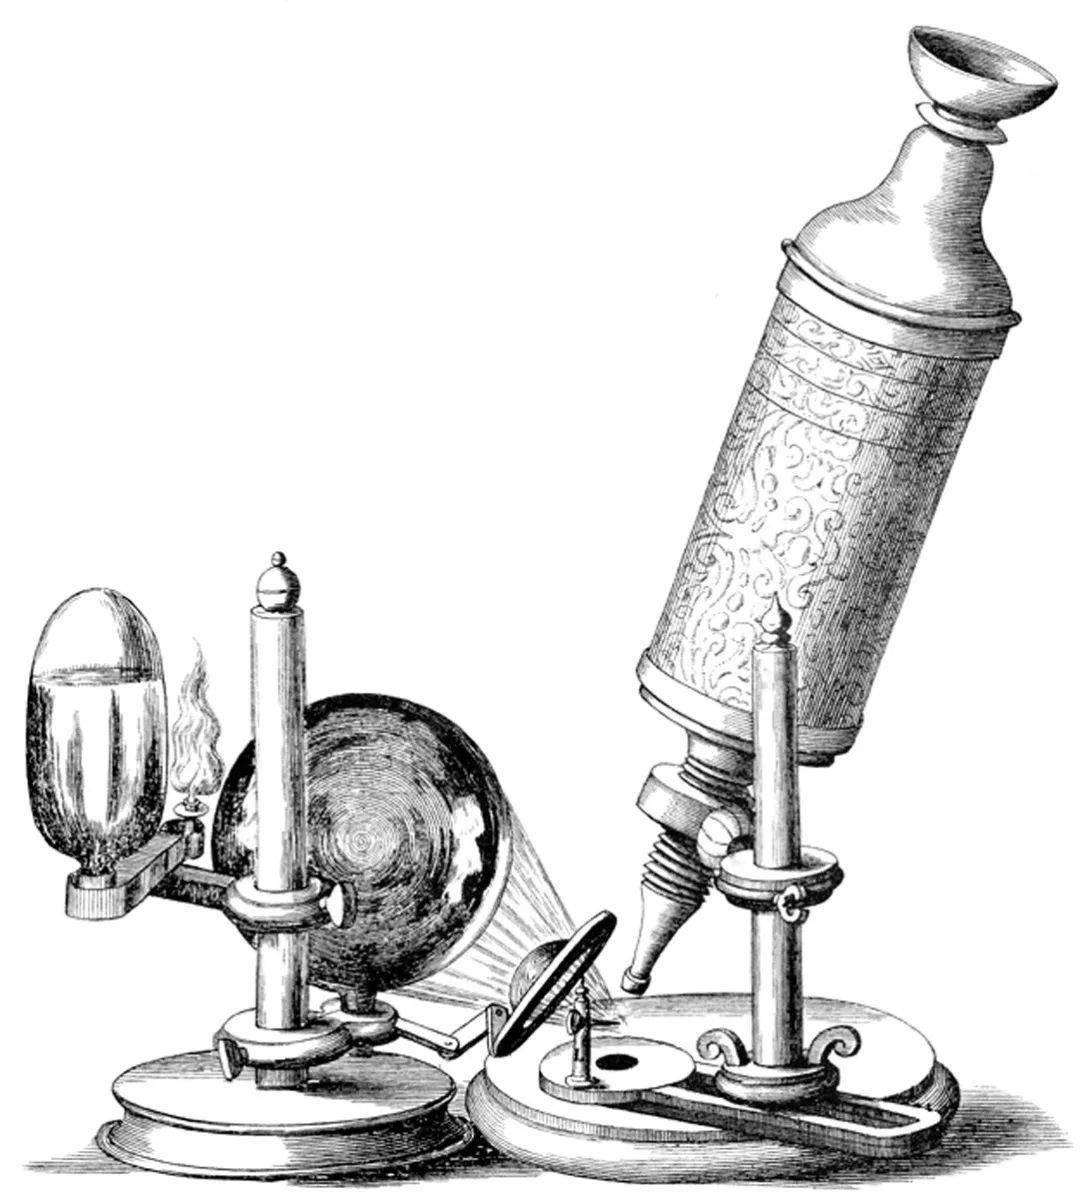
\includegraphics[width=\linewidth]{fig1.jpeg}
			\caption{Robert Hooke 制作的复合显微镜}
		\end{subfigure}%
		\hspace*{\fill}   % maximize separation between subfigures
		\begin{subfigure}{0.31\textwidth}
			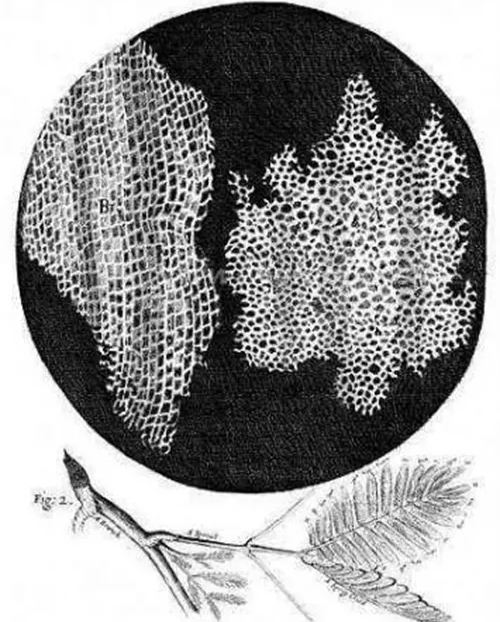
\includegraphics[width=\linewidth]{fig2.png}
			\caption{Robert Hooke 观察栎树皮薄片}
		\end{subfigure}
		\hspace*{\fill}   % maximizeseparation between subfigures
		\begin{subfigure}{0.31\textwidth}
			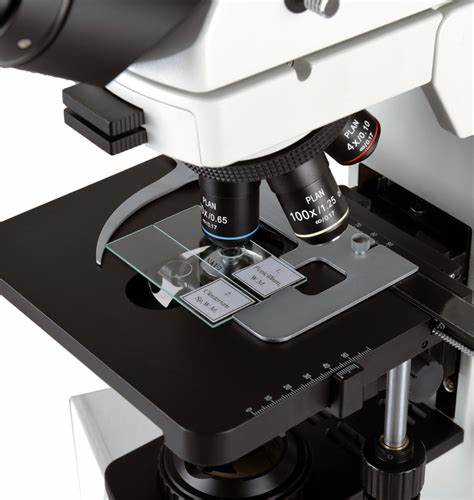
\includegraphics[width=\linewidth]{fig3.png}
			\caption{现代光学显微镜}
		\end{subfigure}
		\caption{显微镜的发展历史:光学显微镜}
	\end{figure}
	\vskip 1em
	
	
	\subsubsection[电子显微镜]{电子显微镜}
	\begin{itemize}
		\item 1930 年:德国科学家 Ernst August Friedrich Ruska 和 Max Knoll 开发了电子显微镜,首次实现了对生物样本的亚显微结构观察。
		\item 20世纪30年代,两位德国物理学家 Max Knoll 和 Ernst Ruska 开发了世界上第一台投射电子显微镜(TEM)。电子显微镜检查电子束和样品之间的相互作用并转化为图像,其分辨率可达到纳米级。
		\item 1937 年, Baron Manfred von Ardenne 对 TEM 的设计进行了改进,建立了扫描电子显微镜(STEM)。STEM 使用一束电子在试样表面扫描并收集产生的"反向散射",可以依此生成高分辨率、清晰的试样三维图像。
	\end{itemize}
	
	\vskip 1em
	\begin{figure}[htbp]
		\begin{subfigure}{0.45\textwidth}
			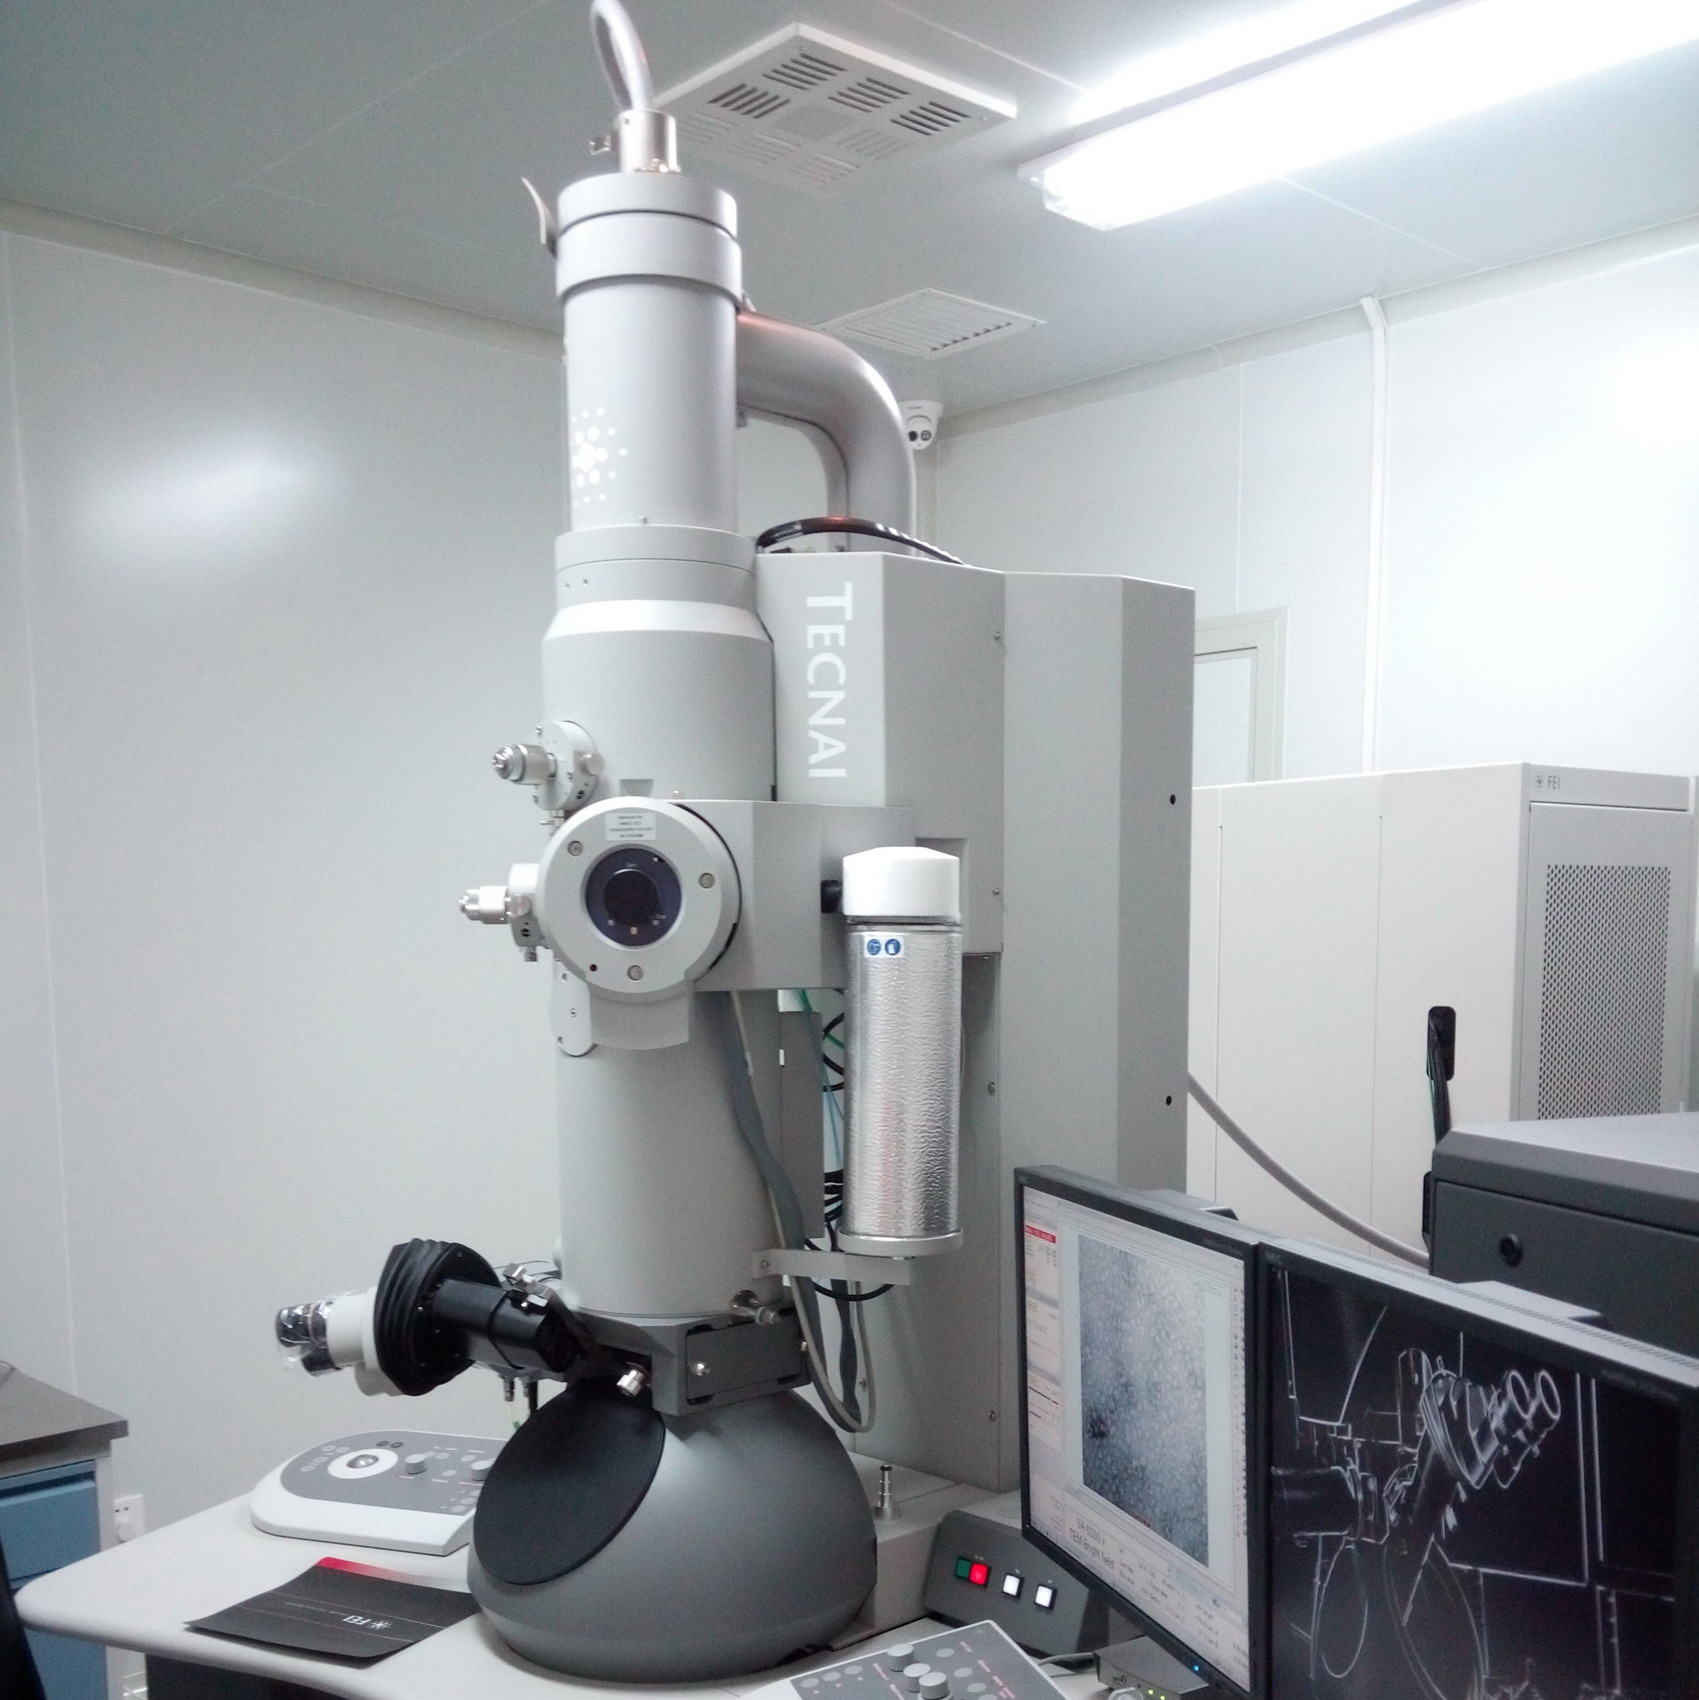
\includegraphics[width=\linewidth]{fig4.jpg}
			\caption{投射电子显微镜(TEM)}
		\end{subfigure}%
		\hspace*{\fill}   % maximize separation between subfigures
		\begin{subfigure}{0.45\textwidth}
			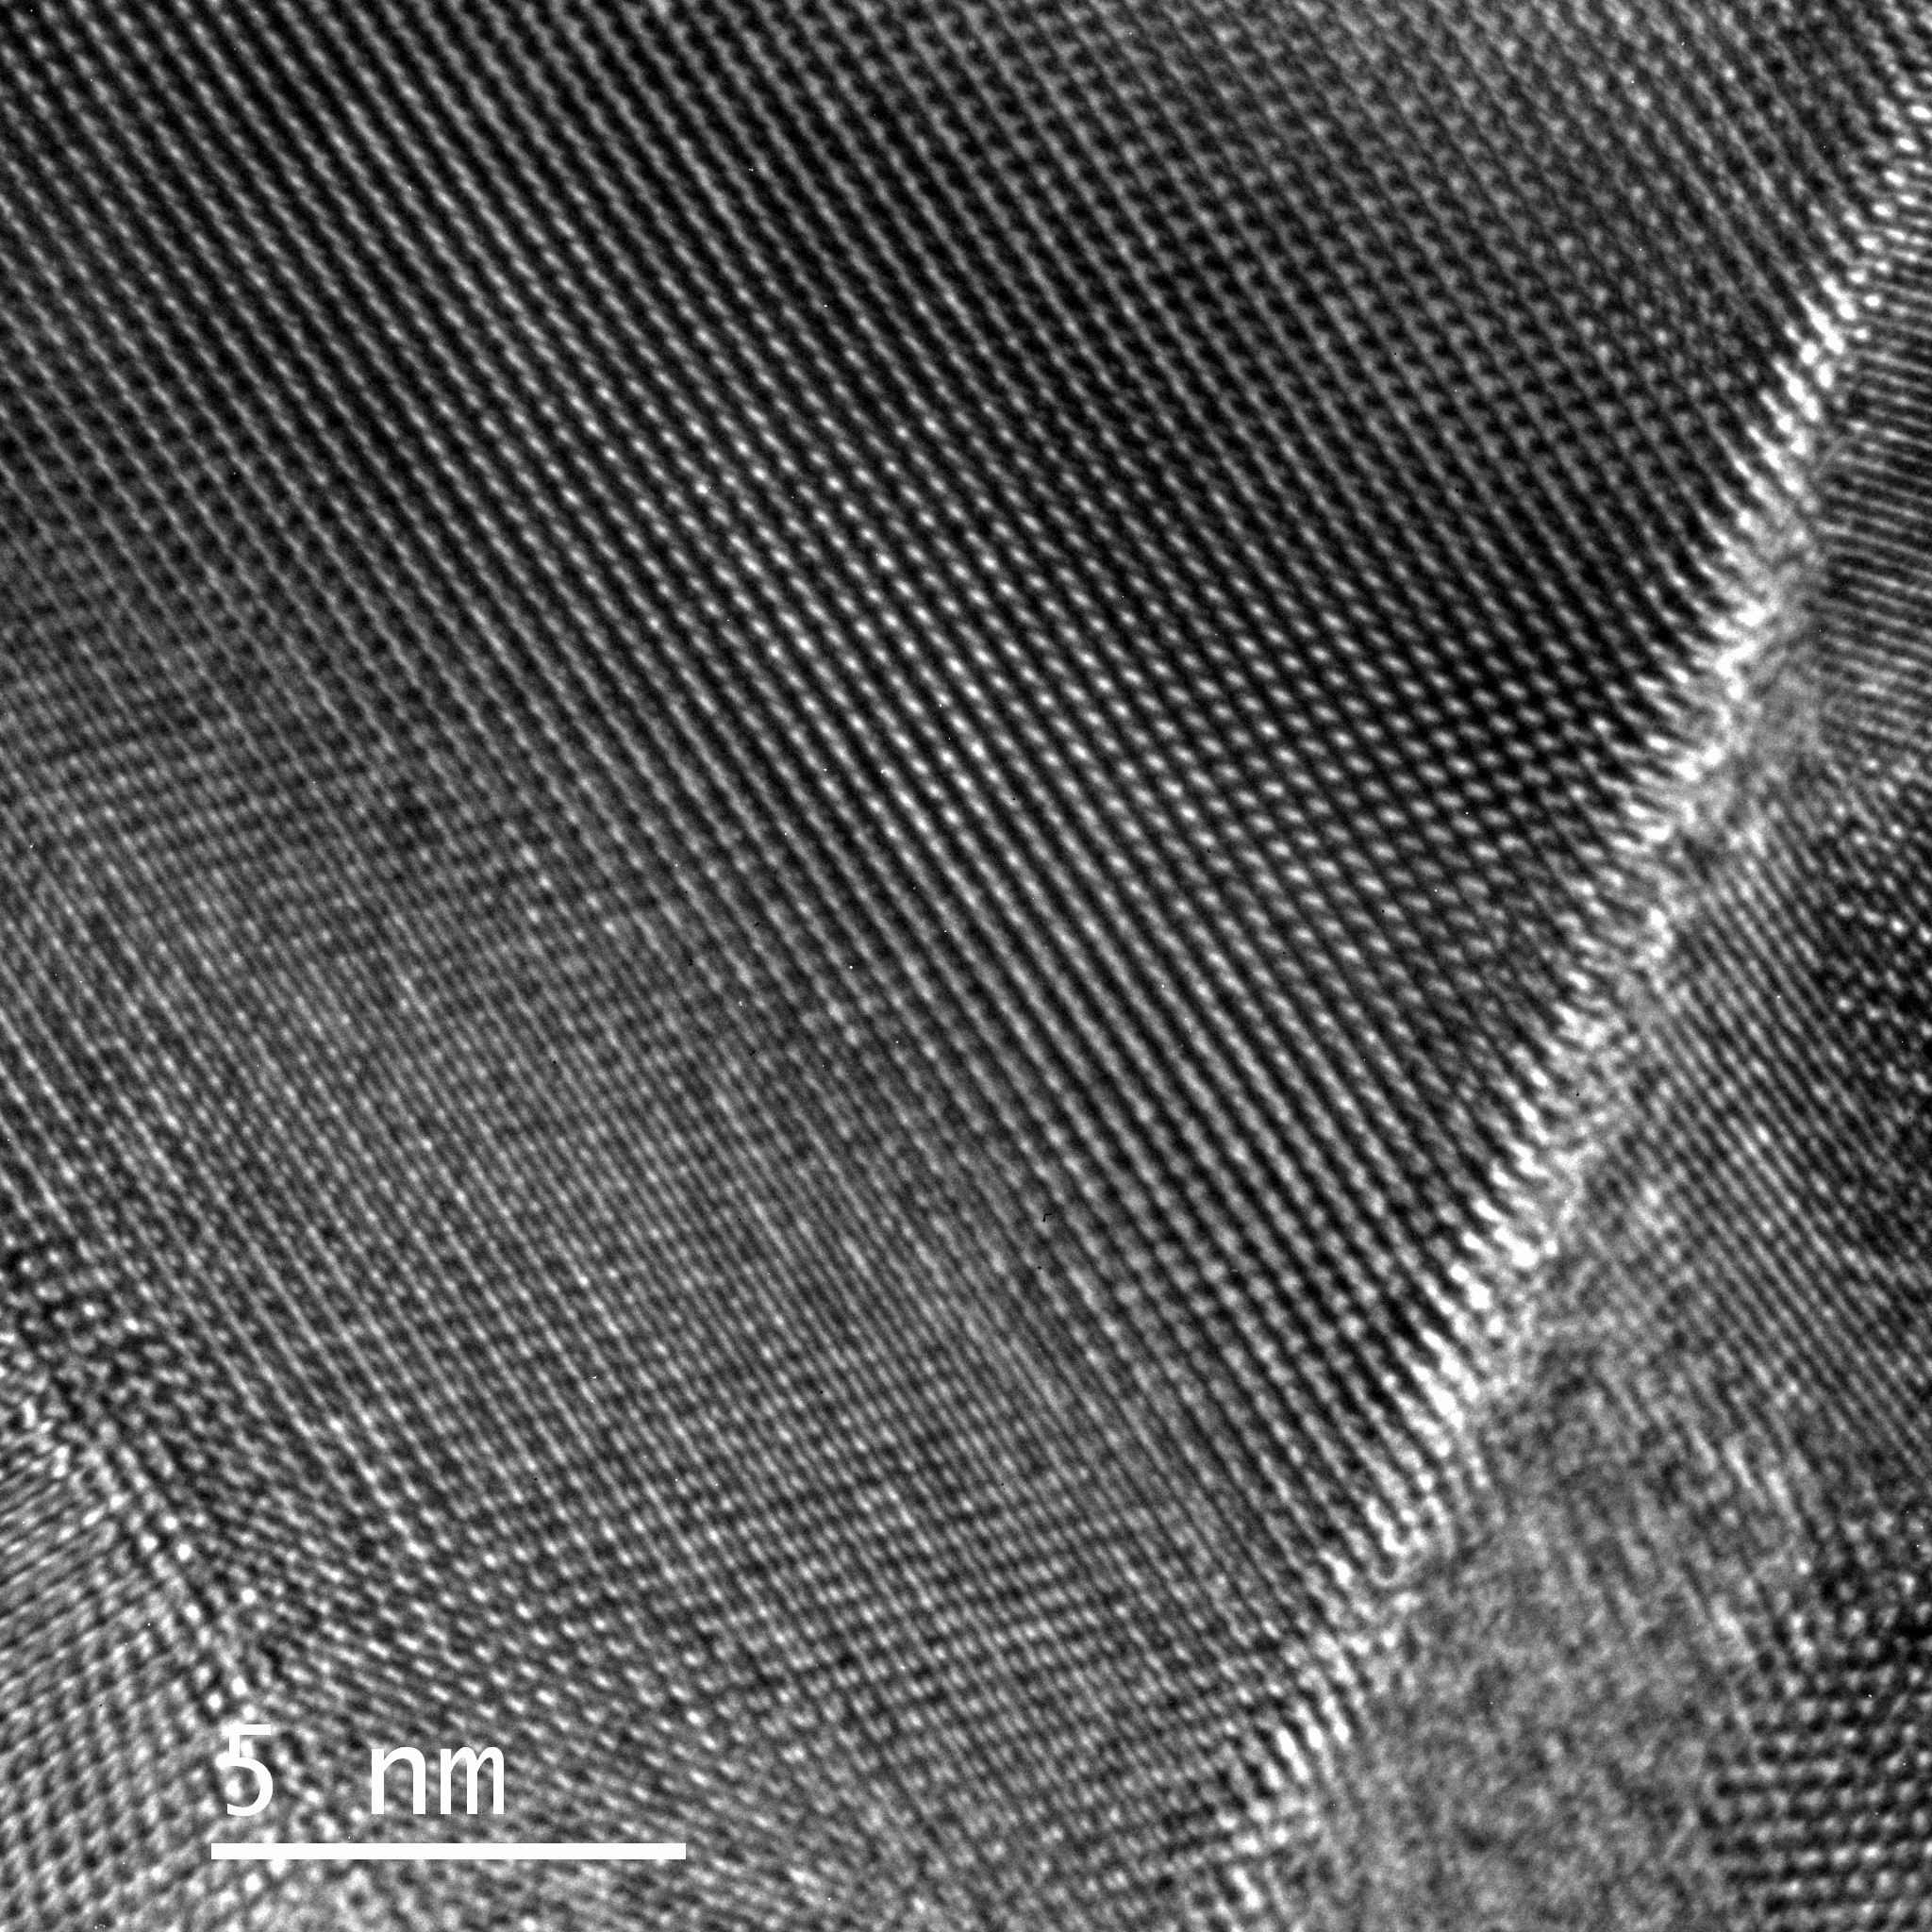
\includegraphics[width=\linewidth]{fig5.jpg}
			\caption{TEM 测试图样}
		\end{subfigure}
		\caption{显微镜的发展历史:电子显微镜}
	\end{figure}
	\vskip 1em
	
	
	
	\subsubsection[扫描隧道显微镜与原子力显微镜]{扫描隧道显微镜与原子力显微镜}
	\begin{itemize}
		\item 1981 年, Gerd Binning 和 Heinrich Rohrer 发现了量子隧穿(QT)现象的发现,并依此建立了第一台扫描隧道显微镜(STM)。STM 克服了光镜和电子显微镜需要光源的缺点,可以达到原子级分辨率。
		\item 1986 年,Gerd Binning,Calvin Quate 和 Christoph Gerber 共同发明了原子力显微镜(AFM),其利用针尖与样品原子之间的范德华力(Van Der Waals Force)的变化来反映样品的表面特性,弥补了 STM 只能用于导体和半导体的不足。
	\end{itemize}
	
	如今在 STM 和 AFM 的基础上,已经衍生出一个庞大的扫描探针显微镜(SPM)家族,广泛用于微观的表面光、磁、热、化学等性质的研究,以及微观生物体系的研究。
	
	
	\subsection{STM 的研究现状与市场现有产品分析}
	%		\setParDis %设置段间距为 0
	\subsubsection[STM 研究现状]{STM 研究现状}
	扫描隧道显微镜自 1981 年发明以来,已经成为纳米科学领域研究不可或缺的重要工具。与此同时,如低温扫描隧道显微镜(LT-STM)等在特殊条件下工作的显微镜也有所发展\cite{ref5,ref6,ref7}。
	
	LT-STM 通过将 STM 装置置于极低温条件下,利用冷冻原子原理来限制样品表面原子的移动或振动。由于样品表面的原子不会因为热运动而移动,从而提高了 STM 扫描成像的精确度和可重复性\cite{ref8}。
	
	此外,有关 STM 在极端环境下的应用同样有所研究\cite{ref1,ref2,ref3}。如美国康奈尔大学的 JC.Seamus Davis等人\cite{ref4},利用 STM 开展了在极低温和强磁场环境下对某些先进功能性材料的研究。近年来,石墨烯作为新型热门材料,可以在极端环境下使用 STM 研究其量子霍尔效应等。
	
	国内对于 STM 的相关研究也有一定的进展:继 2013 年加拿大阿尔伯塔大学教授 Frank Hegmann 首次将太赫兹脉冲和 STM 结合,实现了亚皮秒时间分辨和纳米空间分辨后,其他国家也纷纷开展相关研究。中国科学院空天信息研究院(广州园区)-广东大湾区空天信息研究院成功研制出国内首套自主研制的太赫兹扫描隧道显微镜(THz-STM)系统,实现了埃级的空间分辨率和优于 500 飞秒的时间分辨率,为进一步研究微纳尺度下电子的超快动力学过程、新型量子材料、超快化学等领域提供了有力工具\cite{ref9}。
	
	\begin{figure}[htbp]
		\centering 
		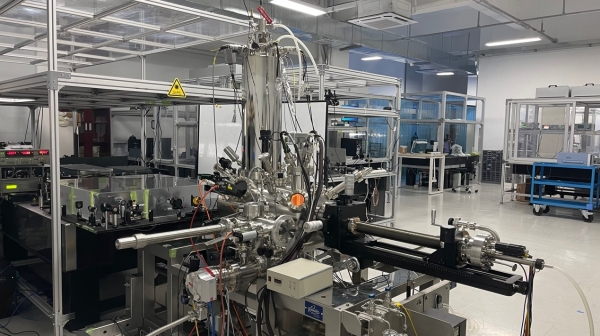
\includegraphics[width=0.8\textwidth]{fig7.png}
		\caption{THz-STM 系统}
	\end{figure}
	
	北京凝聚态物理国家研究中心高鸿钧研究团队与物理所技术部郇庆/刘利团队密切合作,成功研制并搭建了一台多探针 STM 分时复用切换系统,可以完成单个 STM 控制系统操纵多个探针,实现了多探针在纳米尺度下的成像与定位,以及维持探针位置后的局域电输运测量\cite{ref10},为测量材料的电输运性质等提供有效方案。
	
	
	
	\subsubsection[市场现有 STM 产品分析]{市场现有 STM 产品分析}
	市场现有的扫描隧道显微镜产品主要集中于科研和高端工业应用。由于其能够提供原子级别的表面成像和分析能力,STM在纳米科学、表面科学、材料科学等领域具有重要的应用价值。如下列出了几款商品 STM 产品报价:
	\begin{itemize}
		\item Scienta Omicron - STM 产品:一套最基本的配置可能在三四百万元左右,如果加上低温设备等额外功能,价格可能会超过五百万。
		\item 格物致寒(苏州)科学仪器有限公司 - GW415(低温冷却系统)、DRY\_STM\_558(扫描隧道显微镜):整体报价在 300 万元左右。
		\item 布鲁克(北京)科技有限公司 - Multimode 8E 扫描电化学隧道显微镜:报价在 90 万元左右。
	\end{itemize}
	
	
	对市场现有的 STM 产品分析发现,现有 STM 产品通常具有高技术含量和高成本的特点,主要面向对象为科研机构和高端工业用户。随着纳米技术的发展和应用领域的扩大,STM 产品的市场需求预计将持续增长。同时,随着技术的进步和成本的降低,STM 系统可能会逐渐向更多的工业应用和教育领域渗透。
	
	
	
	\subsection{自制 STM 项目的相关研究现状}
	目前互联网上能查找到的最早的自制 STM 项目是 John Alexander 在 2000 年公布的 Simple STM Project\cite{ref12}。该项目有着低成本、易于构建的特点。其中一项关键技术源自于他在 1992 年提交的一篇专利,该专利描述了一种盘状扫描器来控制探针的移动。通过对盘状扫描器上压电陶瓷的四个分区施加不同的电压可以实现探针在三维空间内的精确移动\cite{ref13}。由于该扫描头设计具有成本极其低廉、结构十分简单、易于制作等特点而受到后续诸多 DIY STM 项目的青睐。
	
	2017 年,加拿大麦吉尔大学的博士生 Dan Berard 在家中成功自制了一台 STM,并用它拍摄到了石墨碳原子的图像(图 \ref{fig0})\cite{ref11}。他的自制 STM 成本仅为大约 1000 美元,远低于市场上专业 STM 设备的价格。这一项目的成功展示了个人自制 STM 的可能性,为构建用于科学研究和教育的低成本 STM 提供了解决思路。
	
	\begin{figure}[!htbp]
		\centering
		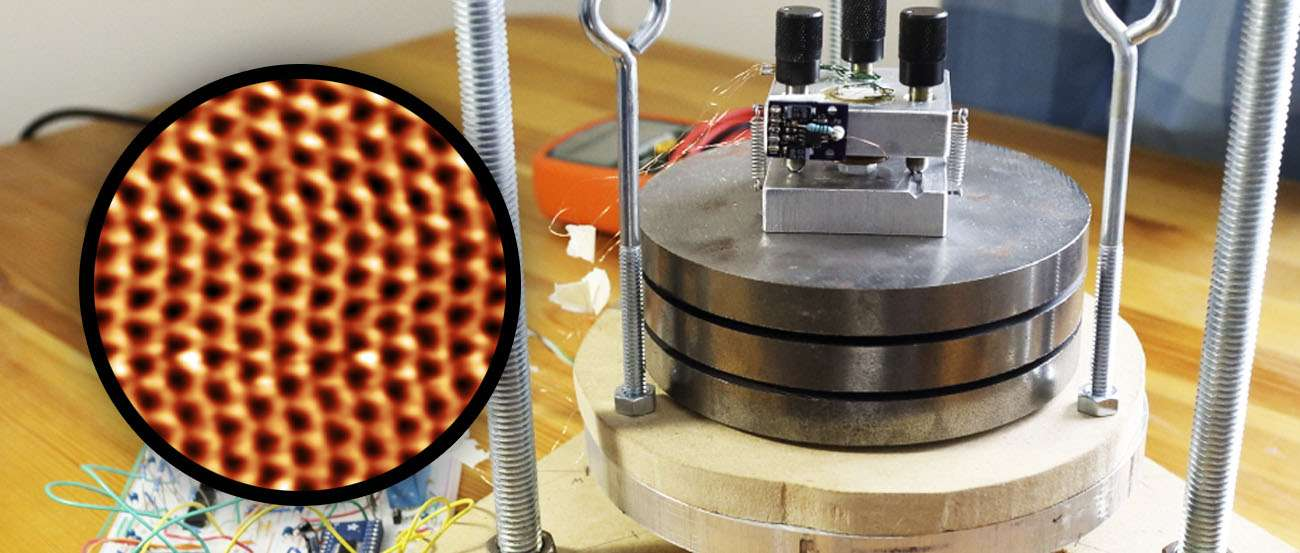
\includegraphics[width=0.8\textwidth]{fig0.png}
		\caption{Dan Berard 的自制 STM 与获得的碳原子图像}
		\label{fig0}
	\end{figure}
	
	截至目前,有关自制 STM 的项目仍然较少,其发展仍然处于起步阶段。由于技术等原因,目前专业 STM 成本与售价仍然较高,部分科研人员、教育工作者和学生仍然难以接触到真正的 STM。因此,构建一种成本足够低、复现简单、易于操作的 STM 在科研与教育领域具有十分重要的意义。
	
	
	
	
	
	
	
	\clearpage
	\section{STM 简介}
	\setParDis %设置段间距为 0
	\subsection{量子隧穿效应与 STM 基本原理}
	为了逐步理解量子隧穿效应,我们首先研究粒子在经典物理下的行为。为了简化描述,我们只考虑粒子的一维运动。此时粒子的运动可以被如下方程所描述:
	\begin{align*}
		E_k = \dfrac{1}{2}mv^2 = E - E_p(z)
	\end{align*}
	其中 $E_k$、$E$ 和 $E_p$ 分别表示粒子的动能、粒子的总能量和粒子在某一点的势能。当 $E - E_p(z) \geq 0$ 时,$v$ 存在实数解;当 $E - E_p(z) < 0$ 时,$v$ 不存在实数解。因此,粒子将无法到达与越过 $E - E_p(z) < 0$ 的区域(即粒子无法跨越势垒)。
	
	\begin{figure}[htbp]
		\centering
		\begin{tikzpicture}
			%					\draw[help lines, color=black!50, step=1cm,very thin](-5,0)grid(5,4);
			%					\draw [fill=black] (-5,0)circle(.1cm);
			
			\draw [->,ultra thick, color=black](-5,0)--(5,0);
			\draw [->,ultra thick, color=black](-5,0)--(-5,4);
			\node at (-5,4)[right]{$Energy$};
			\node at (5,0)[below]{$z$};
			
			\draw [line width=2pt, color=green](-5,0.06)--(-1,0.06);
			\draw [line width=2pt, color=red](-1,0.06)--(4,0.06);
			\draw [dashed,very thick,color=black](-5,0.5)--(-5,-0.5);
			\draw [dashed,very thick,color=black](-1,0)--(-1,-0.5);
			\draw [dashed,very thick,color=black](4,0)--(4,-0.5);
			\node at (-3,0)[below]{可到达区域};
			\node at (1.5,0)[below]{不可到达区域};
			
			\draw [ultra thick, color=blue](-5,0.5)--(-1,0.5)--(-1,3)--(1,3)--(1,0.5)--(4,0.5);
			\draw [ultra thick, color=black](-5,1.5)--(-1,1.5);
			\draw [dashed, ultra thick, color=black](-2,1.5)--(4,1.5);
			\node at(4,1.5)[above]{$E$};
			\node at(4,0.5)[above]{$E_p$};
			\node at(0,3)[above]{势垒};
			
			\draw [<->,ultra thick, color=black](-4.5,0.5)--(-4.5,1.5);
			\node at(-4.5,1)[right]{$E - E_p(z) \geq 0$};
			\draw [<->,ultra thick, color=black](-1.3,1.5)--(-1.3,3);
			\draw [dashed,very thick, color=black](-1.6,3)--(-1,3);
			\node at(-1.3,2.3)[left]{$E - E_p(z) < 0$};
			
		\end{tikzpicture}
		\caption{经典物理体系下系统能量示意图}
	\end{figure}
	
	
	20 世纪初,量子力学的出现彻底改变了人们对物质的理解方式。在量子力学中,粒子将可以跨过传统物理中不可逾越的“高山”。1926 年,奥地利物理学家 Erwin$\,$ Schr$\mathop{\text{o}}\limits^{..}$dinger 提出了 Schr$\mathop{\text{o}}\limits^{..}$dinger 方程,用于描述粒子在量子力学中的行为。它是一个二阶二元微分方程,但在理解隧穿效应的过程中,时间 t 并非必需的,因此我们引入如下简化的 Schr$\mathop{\text{o}}\limits^{..}$dinger 方程(也即一维不含时 Schr$\mathop{\text{o}}\limits^{..}$dinger 方程):
	\begin{align*}
		\dfrac{d^2\psi(z)}{dz^2} = -\dfrac{2m}{\hslash^2}(E-E_p)\psi(z)
	\end{align*}
	其中 $\hslash=\dfrac{h}{2\pi} =  1.054 \times10^{-34} Js$ 为约化普朗克常数,用于简化方程。通过给定边界条件,我们可以求解出描述系统状态的波函数方程。该波函数与粒子停留在空间某个区域的概率之间存在关系,即:
	\begin{align*}
		P(z) = (\psi(z))^2
	\end{align*}
	
	将 STM 抽象为一维势垒模型(如图 \ref{fig1} 所示),应用 Schr$\mathop{\text{o}}\limits^{..}$dinger 方程并结合边界条件,可以计算出电子的波函数(如图 \ref{fig2} 所示)。
	
	\begin{figure}[!h]
		\centering
		\begin{subfigure}{\textwidth}
			\centering
			\tikz{
				%					\draw[help lines, color=black!50, step=1cm,very thin](-5,0)grid(5,4);
				
				\draw [->,ultra thick, color=black](-5,0)--(5,0);
				\draw [->,ultra thick, color=black](-5,0)--(-5,4);
				\node at (-5,4)[right]{$Energy$};
				\node at (5,0)[below]{$z$};
				
				\draw [dashed,very thick,color=black](-5,0)--(-5,-0.5);
				\draw [dashed,very thick,color=black](-1,0)--(-1,-0.5);
				\draw [dashed,very thick,color=black](1,0)--(1,-0.5);
				\draw [dashed,very thick,color=black](4,0)--(4,-0.5);
				\node at (-3,0)[below]{样品};
				\node at (0,0)[below]{真空};
				\node at (2.5,0)[below]{针尖};
				
				\draw [ultra thick, color=blue](-5,0.5)--(-1,0.5)--(-1,3)--(1,3)--(1,0.5)--(4,0.5);
				\draw [ultra thick, color=red](-5,1.5)--(-1,1.5);
				\draw [ultra thick, color=red](1,1.5)--(4,1.5);
				\node at(4,1.5)[above]{$E$};
				\node at(4,0.5)[above]{$E_p$};
				\node at(0,3)[above]{势垒};
				
				\draw [<->,ultra thick, color=black](-1.3,1.5)--(-1.3,3);
				\draw [dashed,very thick, color=black](-1.6,3)--(-1,3);
				\node at(-1.3,2.3)[left]{$\phi$};
				
			}
			\caption{STM 的势垒模型}
			\label{fig1}
		\end{subfigure}
		\vskip 1em
		\begin{subfigure}{\textwidth}
			\centering
			\tikz{
				%					\draw[help lines, color=black!50, step=1cm,very thin](-5,-2)grid(5,3);
				
				\draw [->,ultra thick, color=black](-5,0)--(5,0);
				\draw [->,ultra thick, color=black](-5,-2)--(-5,3);
				\node at (-5,3)[right]{$\psi$};
				\node at (5,0)[below]{$z$};
				
				\draw [dashed,very thick,color=black](-5,-2)--(-5,3);
				\draw [dashed,very thick,color=black](-1,-2)--(-1,3);
				\draw [dashed,very thick,color=black](1,-2)--(1,3);
				\draw [dashed,very thick,color=black](4,-2)--(4,3);
				\node at (-3,-1.8)[below]{样品};
				\node at (0,-1.8)[below]{真空};
				\node at (2.5,-1.8)[below]{针尖};
				
				\draw[smooth,samples=50,very thick,color=black,domain=-5:-1] plot(\x,{1.7*sin(2*(\x-1.2) r)});
				\draw [smooth,very thick,color=black](-1,1.6) ..controls(0,0.75)..(1,0.5);
				\draw[smooth,samples=50,very thick,color=black,domain=1:4] plot(\x,{0.5*sin(2.5*(\x-0.4) r)});
				
			}
			\caption{粒子的波函数示意图}
			\label{fig2}
		\end{subfigure}
		\caption{量子力学体系下系统状态示意图}
	\end{figure}
	
	分析 $\psi(z)$ 可以发现,在势垒的另一侧仍然存在 $P(z)=(\psi(z))^2 > 0$。这说明在量子力学体系下,电子将不再被“禁锢”于势垒的一侧,而是有概率穿过势垒,到达势垒的另一侧。然而此时仍不存在隧穿电流,因为势垒两侧不存在电压差,两侧电子穿过势垒的概率相等。当施加一定电压后,处于高电位一侧的电子将会有更大概率通过势垒,从而产生一个微弱的隧穿电流。通过一定推导,我们可以得出隧穿电流的大小和样品表面与针尖的距离成指数关系,即:
	\begin{align*}
		I \propto e^{-kd}
	\end{align*}
	其中 I 为隧穿电流的大小,d 为样品表面与针尖的距离。这表明当距离发生微小变化时,隧穿电流将会产生较大变化。这种变化十分灵敏,是 STM 达到原子级分辨率的关键。
	
	
	
	
	
	\subsection{STM 的关键组件与功能}
	\begin{figure}[htbp]
		\centering 
		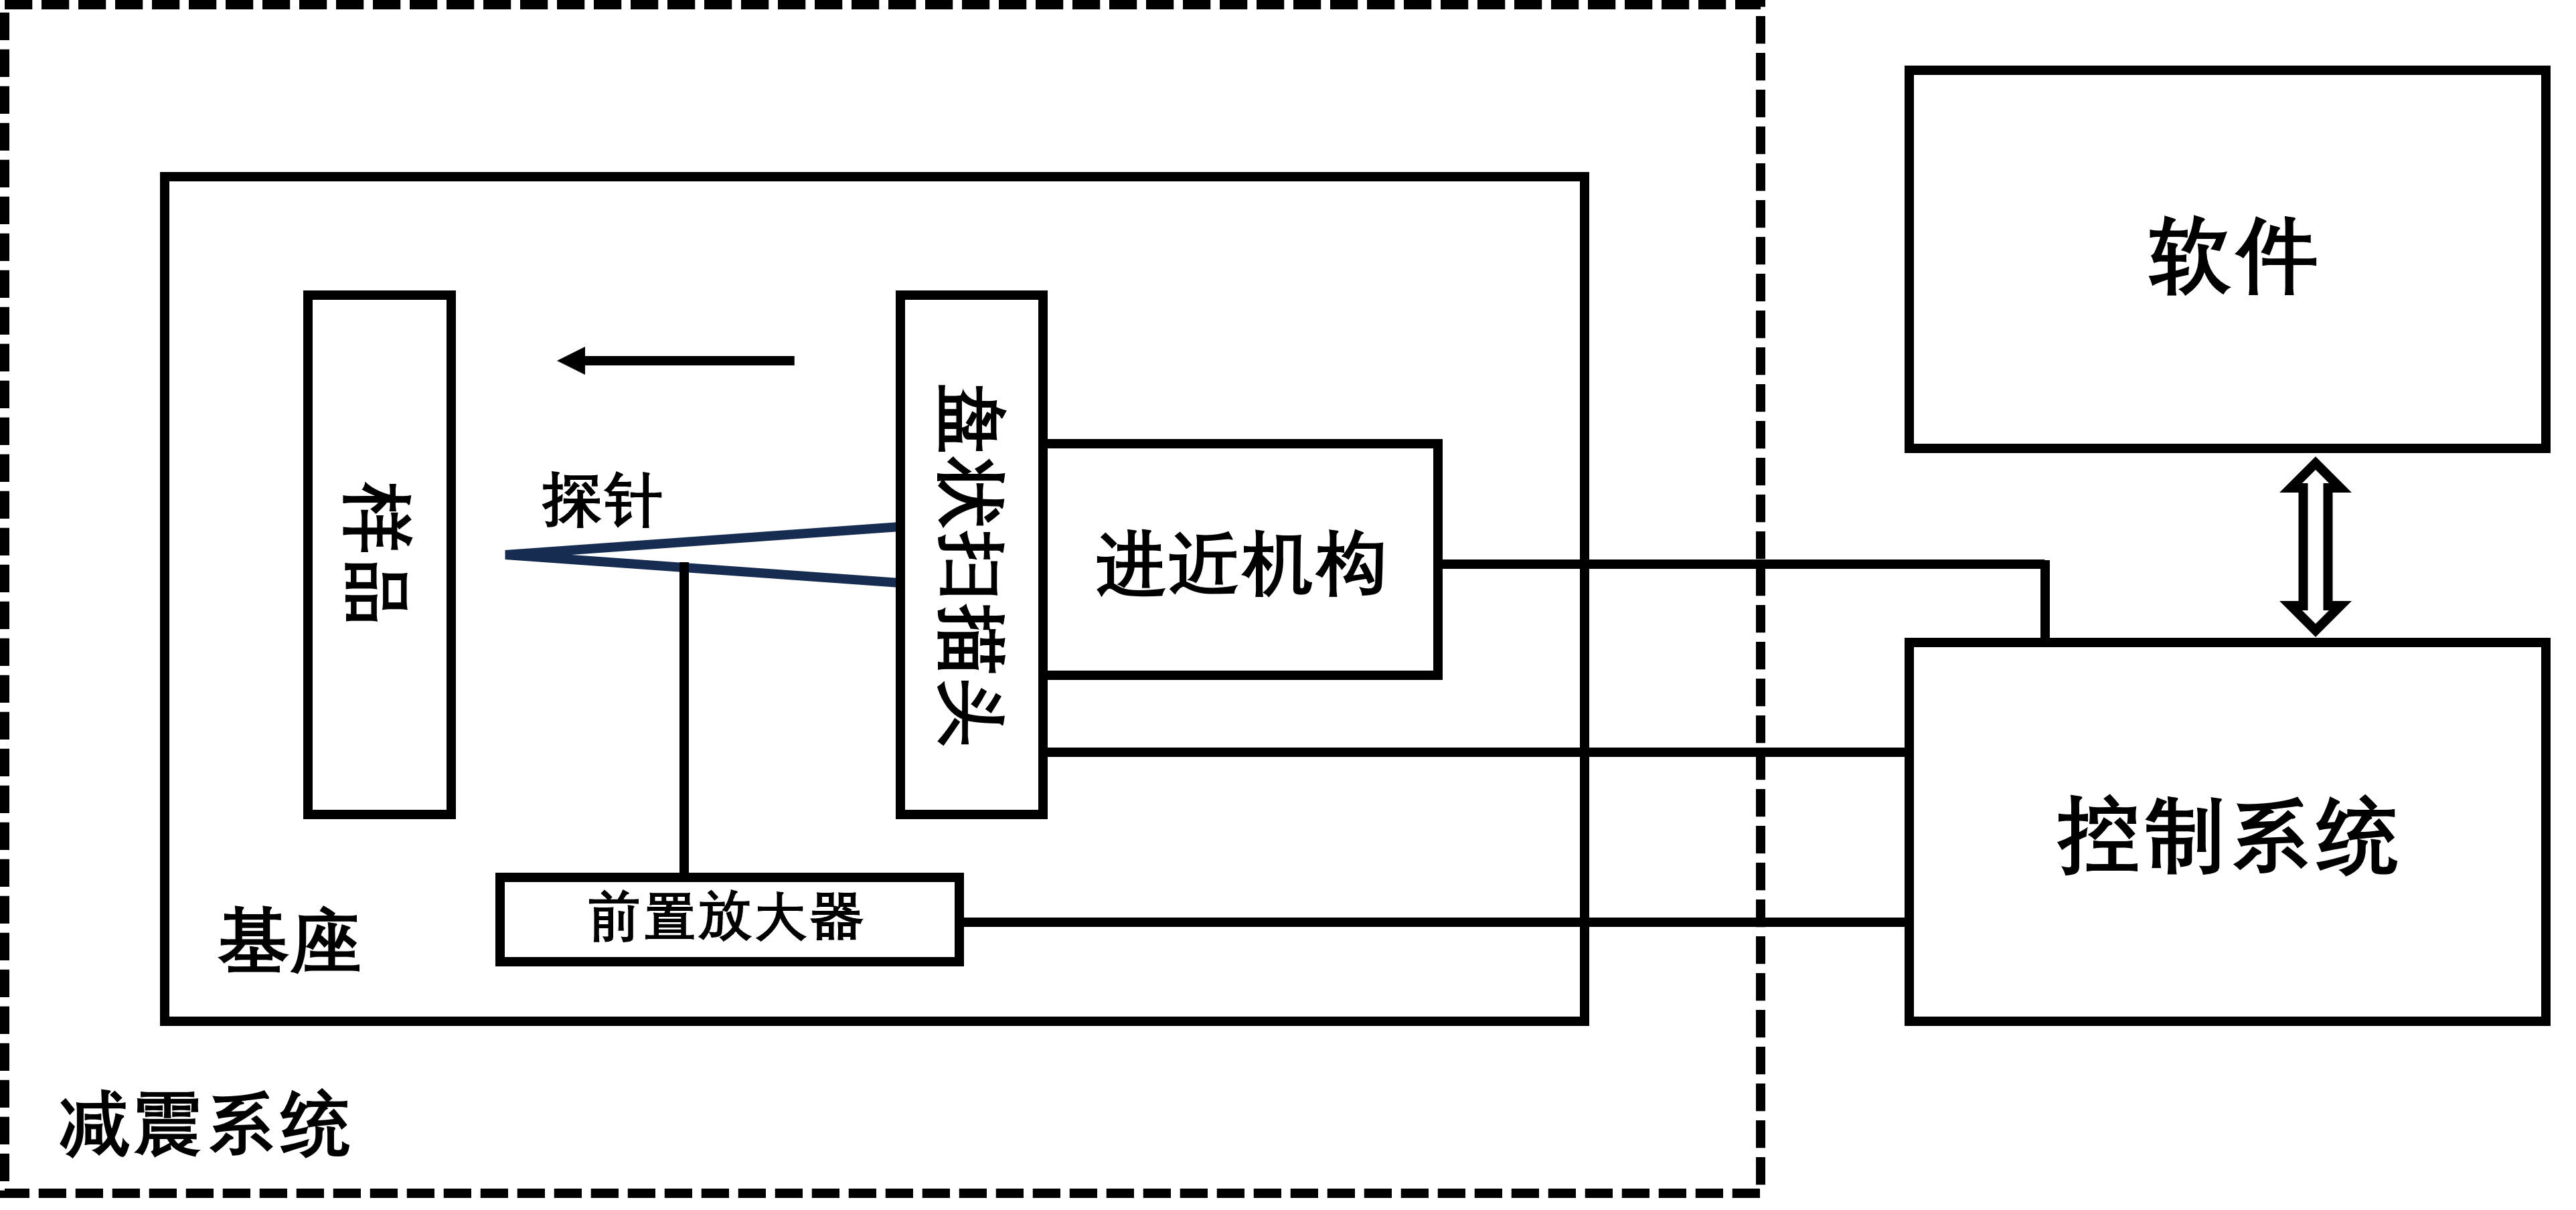
\includegraphics[width=0.8\textwidth]{fig8.png}
		\caption{STM 系统的关键组件示意图}
	\end{figure}	
	一般来说,扫描隧道显微镜的关键组件及其功能如下:
	\begin{enumerate}
		\item \textbf{探针}\par
		\qquad 探针是 STM 的核心部件,通常由尖锐的金属丝(如钨丝或铂丝)制成。探针的尖端极度尖锐,甚至只有一个或几个原子的大小,其用于接近样品表面至足以产生量子隧道效应的距离。
		
		\item \textbf{样品}\par
		\qquad 样品必须是可导电的,以便在探针和样品之间产生隧穿电流。样品被固定在 STM 的磁性样品台上,可以进行精确的移动和定位。
		
		\item \textbf{探针控制系统}\par
		\qquad 探针控制系统主要包含压电陶瓷扫描器和粗进近机构两个部分。压电陶瓷扫描器:利用逆压电效应精确地控制探针在 X、Y、Z 方向上的位移,从而实现探针在样品表面的精确扫描;粗进近机构:由于压电陶瓷的位移量较小,需要通过其他机械结构将探针推进至压电陶瓷扫描器的可控制范围内。
		
		\item \textbf{反馈控制系统}\par
		\qquad 该系统可以实时监测隧穿电流,并根据隧穿电流的变化自动调整探针与样品之间的距离,以保持恒定的隧道电流(或恒定的距离)。
		
		\item \textbf{真空系统}\par
		\qquad STM 通常在真空或惰性气体环境中操作,以减少空气等对扫描精度的影响。
		
		\item \textbf{减震系统}\par
		\qquad 减震系统用于减小高频震动对形成稳定隧穿电流的影响,保证探针与样品表面维持稳定的距离。
		
		\item \textbf{温控系统}\par
		\qquad 该系统维持 STM 的工作温度以减小温漂对维持稳定隧穿电流的影响。
		
		\item \textbf{数据处理与控制软件}\par
		\qquad 用于分析和显示 STM 采集的数据,将探针扫描得到的隧穿电流信号转换成样品表面的三维图像以及操作 STM。
		
	\end{enumerate}
	
	
	
	
	
	
	
	
	
	
	\clearpage
	\section{自制 STM 的技术难点与初步解决方案}
	\setParDis %设置段间距为 0
	
	\begin{enumerate}
		\item \textbf{制备纳米级锐度的探针}\par
		\qquad 探针的针尖应当尽可能尖锐,因为只有当隧穿电流仅从针尖的几个原子通过时,STM 的分辨率才能达到最高。通常专业级 STM 探针使用化学蚀刻法取得良好锐度的探针,但是这种方法成本较高且操作难度较大,不适用于自制 STM 项目。图 \ref{fig5} 展示了普渡大学手工裁剪 Pt/Ir 丝后获得的针尖的透射电子扫描图像\cite{ref19}。研究人员通过使用洁净的工具直接剪切 Pt/Ir 丝来获得 STM 针尖。通常情况下此法取得的针尖形状并不规则,有时会产生多个尖端。然而此方法有几率获得极度锐利的针尖。尽管不能保证每次裁剪都获得足够尖锐的针尖,但其不失为一种简单、成本低廉地获得 STM 针尖的有效方法。
		
		\begin{figure}[!h]
			\centering
			\begin{subfigure}{0.35\linewidth}
				\centering
				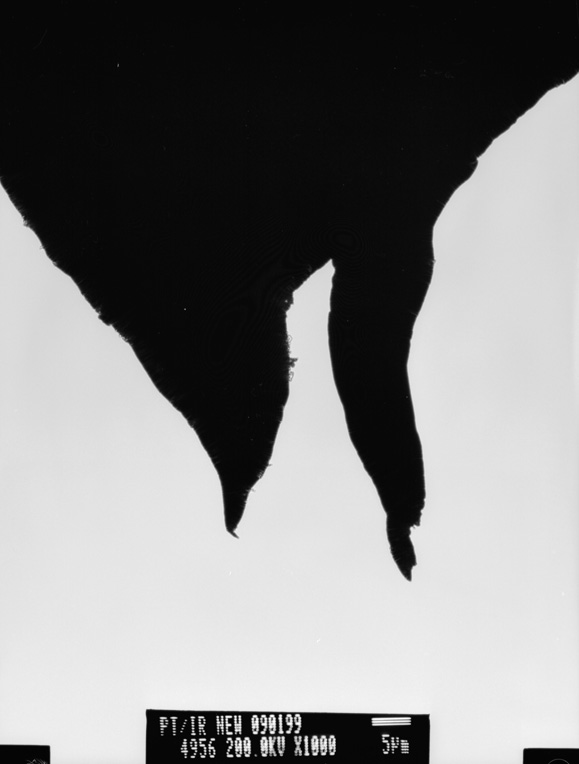
\includegraphics[height=7.5cm]{fig1.jpg}
				\caption{Pt/Ir, 0.008" diameter\\\quad}
			\end{subfigure}
			\hskip 1.5cm
			\begin{subfigure}{0.35\linewidth}
				\centering
				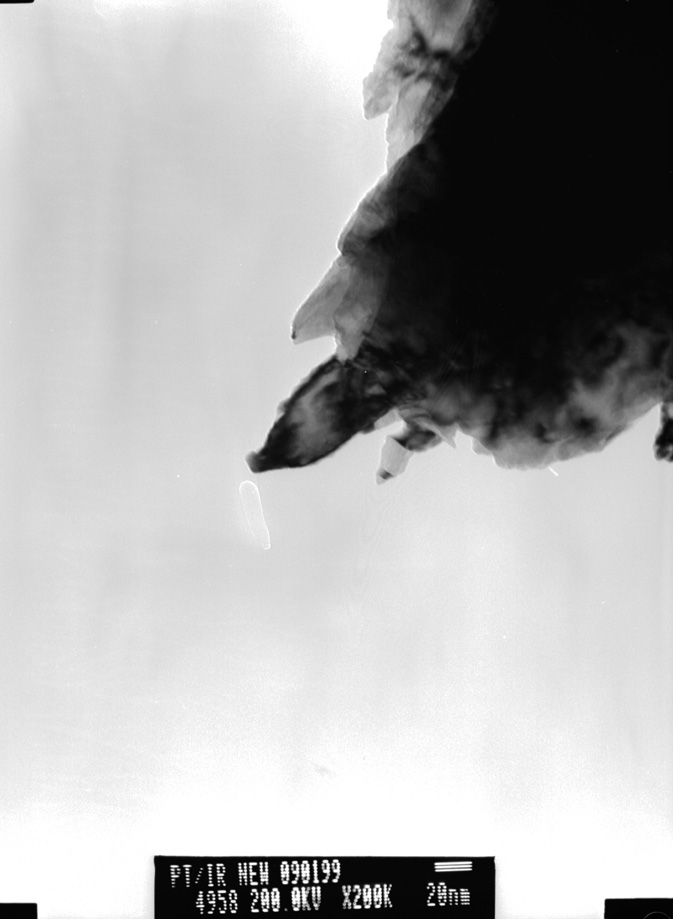
\includegraphics[height=7.5cm]{fig2.jpg}
				\caption{Pt/Ir, 0.008" diameter, Bar length = 20 nm(局部放大)}
			\end{subfigure}
			\caption{手工剪切 STM 针尖的 TEM 图像}
			\label{fig5}
		\end{figure}
		
		
		
		\item \textbf{检测极小的隧穿电流}\par
		\qquad 通常情况下,隧穿电流非常小(通常在 $1\sim10nA$)。为了获得可测量的信号,必须使用前置放大器来预处理针尖流过的隧穿电流。跨阻放大器(TIA)作为一种常见的放大电路,具有高增益、低噪声的优良特性,十分适合作为 STM 的前置放大器。它的核心器件为一个精密运放和一个反馈电阻。当反馈电阻阻值为 $100M\Omega$ 时,它可以将 $10nA$ 的输入电流放大为 $-1V$ 在输出端输出\cite{ref11,ref12,ref17}。同时考虑到外界市电干扰等噪声,应将其用金属包被以屏蔽噪声。
		
		
		
		
		\item \textbf{控制探针实现纳米级移动扫描}\par
		\qquad STM 需要控制探针在样品表面以纳米级尺度进行移动扫描,因此我们需要一种精确可控的方式来实现探针的移动。常见的压电陶瓷横线压电应变常数(图 \ref{tab1})通常在 $0.1V/nm$ 左右,因此利用压电晶体的逆压电效应,即对压电陶瓷施加一定电压即可获得可控的纳米级的位移。
		
		\begin{table}[H]
			\small
			\caption{常见压电陶瓷的横线压电应变常数}
			\centering
			\begin{tabular}{cc}
				\toprule
				\qquad\textbf{压电陶瓷类型}\qquad\qquad &\qquad \textbf{d31(nm/V)} \qquad\qquad  \\ 
				\midrule
				PZT-4	&	-0.12	\\  
				PZT-5A 	& 	-0.18	\\
				PZT-5H 	& 	-0.27	\\
				BM500 	&	-0.16	\\
				BM527	&	-0.25	\\
				\bottomrule
			\end{tabular}\\\vskip 1mm
			\begin{minipage}{0.5\linewidth}
				附注:PZT-4、PZT-5A、PZT-5H 的数据来自于 Morgan Electro Ceramics 公司,BM500、BM527 的数据来自 Sensor Technology 公司。 
			\end{minipage}
			\label{tab1}
		\end{table}
		
		
		
		
		
		\item \textbf{将探针推进至隧穿距离而不发生碰撞}\par
		探针推进过程包含两个阶段:
		\begin{itemize}
			\item \textbf{粗进近阶段}:惯性压电滑台是利用滑台惯性以及粘滑现象实现高精度长距离位移的一种设备,具有精度极高、发热量小等优点,十分适合 STM 进近工作。使用惯性压电滑台可以实现探针的高精度的长距离移动,将探针推进至距离样品几纳米的附近。
			
			\item \textbf{精细进近阶段}:使用惯性压电滑台和压电陶瓷扫描头共同进行更加精细控制。
			
		\end{itemize}
		
		
		
		
		
		\item \textbf{真空环境问题}\par
		\qquad 实际上,STM 可以正常工作在常温常压的空气环境中,真空环境并非成像所必需的。根据 Paschen 定律我们可以得出:使空气发生击穿放电的最小电压为 360 V(图 \ref{fig3}),且随着距离进一步减小击穿电压急剧上升 。而在 2003 年 Al Wallash 与 Larry Levit ,2010 年 Rakshit Tirumala 与 David B. Go 分别对 Paschen  曲线做出修正,得到了极小尺度下更为准确的空气击穿曲线(图 \ref{fig4})\cite{ref14,ref15}。当间隙大于 $5\mu m$ 时,空气击穿依旧由 Townsend 效应主导;而当间隙小于 $5\mu m$ 时,由于间隙极小,间隙两端将产生很强的电场,电子将直接被发射出去(即场发射电流),此时的击穿电压将随着距离的减小进一步降低;而当间隙继续减小至 $2nm$ 左右时,电流的大小将由隧穿效应主导,此时只需很小的电压即可使空气导电。目前已经有多个自制 STM 项目在空气中完成了扫描成像\cite{ref16,ref17},足以说明在常温常压空气环境下扫描的可行性。
		
		\vskip 1em
		\begin{figure}[!h]
			\centering 
			\begin{subfigure}{\textwidth}
				\centering 
				\begin{tikzpicture}
					\draw[help lines, color=black!30, step=1cm,ultra thin](0,0)grid(10,6);
					\draw [->,ultra thick, color=black](0,0)--(11,0);
					\draw [->,ultra thick, color=black](0,0)--(0,7);
					\node at (0,6.5)[right]{击穿电压($V$)};
					\node at (5,-0.5)[below]{间隙距离($\mu m$)};
					\node at (-0.3,0)[below]{0};
					\node at (1,0)[below]{10};
					\node at (2,0)[below]{20};
					\node at (3,0)[below]{30};
					\node at (4,0)[below]{40};
					\node at (5,0)[below]{50};
					\node at (6,0)[below]{60};
					\node at (7,0)[below]{70};
					\node at (8,0)[below]{80};
					\node at (9,0)[below]{90};
					\node at (10,0)[below]{100};				
					
					\node at (0,1)[left]{200};
					\node at (0,2)[left]{400};
					\node at (0,3)[left]{600};
					\node at (0,4)[left]{800};
					\node at (0,5)[left]{1000};
					\node at (0,6)[left]{1200};
					
					\draw [smooth,ultra thick,color=black](0.1,6)..controls(0.12,1.5)and(0.13,1.8)..(1,1.86);
					\draw [smooth,ultra thick,color=black](1,1.86)  ..controls(0.9,1.855)..(10,3);
					
					\draw[loosely dashed,blue,ultra thick](0,1.8)--(11,1.8);
					\node at (10.5,1.8)[above]{360};
					\draw[loosely dashed,blue,ultra thick](0.5,0)--(0.5,1.8);
					\node at (0.5,0)[below]{5};
				\end{tikzpicture}
				\caption{Paschen 曲线示意图}
				\label{fig3}
			\end{subfigure}
			
			\begin{subfigure}{\textwidth}
				\centering 
				\begin{tikzpicture}
					\draw[help lines, color=black!30, step=1cm,ultra thin](0,0)grid(10,6);
					\draw [->,ultra thick, color=black](0,0)--(11,0);
					\draw [->,ultra thick, color=black](0,0)--(0,7);
					\node at (0,6.5)[right]{击穿电压($V$)};
					\node at (5,-0.5)[below]{间隙距离($\mu m$)};
					\node at (-0.3,0)[below]{0};
					\node at (1,0)[below]{10};
					\node at (2,0)[below]{20};
					\node at (3,0)[below]{30};
					\node at (4,0)[below]{40};
					\node at (5,0)[below]{50};
					\node at (6,0)[below]{60};
					\node at (7,0)[below]{70};
					\node at (8,0)[below]{80};
					\node at (9,0)[below]{90};
					\node at (10,0)[below]{100};				
					
					\node at (0,1)[left]{200};
					\node at (0,2)[left]{400};
					\node at (0,3)[left]{600};
					\node at (0,4)[left]{800};
					\node at (0,5)[left]{1000};
					\node at (0,6)[left]{1200};
					
					\draw [smooth,ultra thick,color=black](0,0)
					..controls(0.3,0.3)..(0.5,1.7)
					..controls(0.55,1.83)..(0.8,1.75)
					..controls(1,1.7)..(10,3);
					
					%					\draw[loosely dashed,blue,ultra thick](0,1.8)--(11,1.8);
					%					\node at (10.5,1.8)[above]{360};
					\draw[loosely dashed,blue,ultra thick](0.5,0)--(0.5,1.8);
					\node at (0.5,0)[below]{5};
				\end{tikzpicture}
				\caption{Paschen 曲线(修正)示意图}
				\label{fig4}
			\end{subfigure}
			\caption{空气击穿曲线}
		\end{figure}
		\vskip 1em
		
		
		
		
		
		\item \textbf{隔绝震动}\par
		\qquad 震动会导致 STM 探针针尖与样品表面发生偏移导致测量精度下降。现实生活中我们无法完全避免震动的产生与传播,但实际上只有高频震动才会对 STM 造成较大影响。当震动频率较低时,针尖会与样品同步运动,对 STM 的成像影响甚微。因此我们可以通过构建一个简单的悬挂系统来将系统谐振频率降低到几十赫兹,同时配合磁阻尼加强系统滤除高频震动的能力。
		%			\cite{ref17}
		
		
		\item \textbf{温漂问题}\par
		\qquad 尽管温度变化引起的热胀冷缩现象十分微弱,通常其线度只有几十个微米,但这对于精度要求达到纳米级别的 STM 来说是致命的。为了减小温漂的影响,应尽可能选择热膨胀系数相对较小的材料。与此同时,还应将装置放置于相对恒温处,抛弃发热量较高的步进电机而使用压电滑台,使用亚克力罩隔绝气体对流等来尽量减小温漂带来的问题。
		
		
		\item \textbf{控制成本}\par
		\qquad 自制 STM 的最大优势在于相较于专业 STM 设备其成本低廉、容易制作。因此应尽量保持性能与成本间的平衡,尽可能用最低的成本获得最佳质量的成像。此外,STM 的选材应尽可能选取生活中比较容易获得的材料,以尽可能降低成本与制作难度。
		
	\end{enumerate}
	
	
	
	
	
	
	
	
	
	
	\clearpage
	\section{自制 STM 的设计方案}
	\setParDis %设置段间距为 0
	\subsection{基本组成}
	\begin{figure}[htbp]
		\centering 
		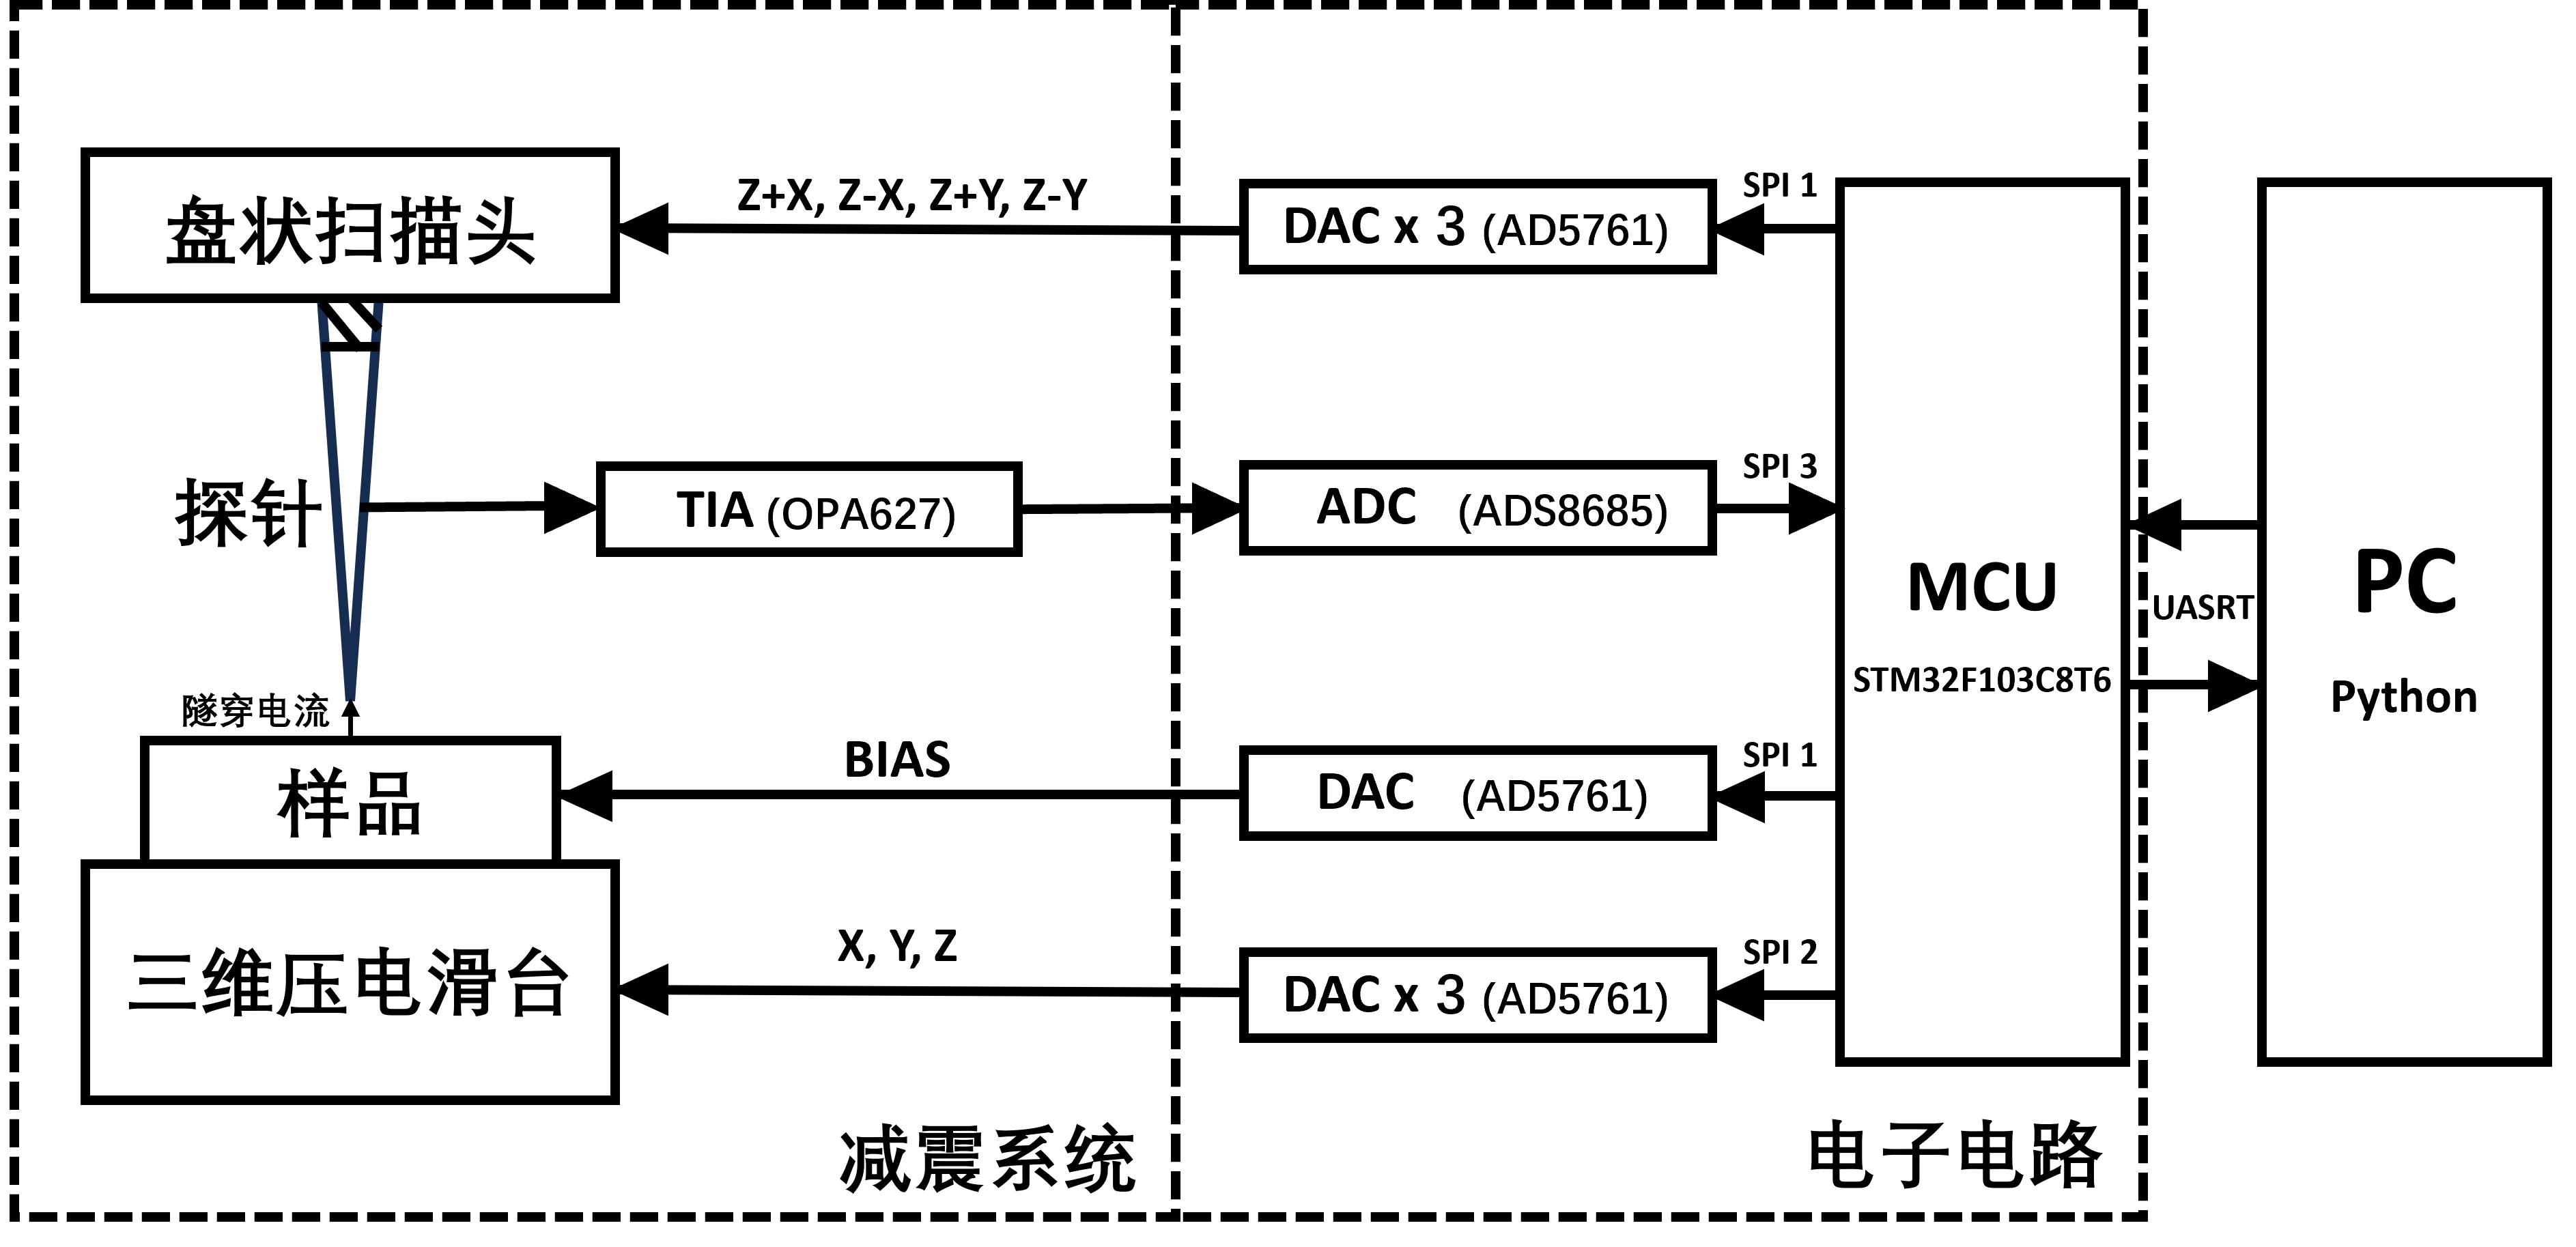
\includegraphics[width=0.8\textwidth]{fig88.png}
		\caption{DIY-STM 设计示意图}
	\end{figure}	
	
	在本设计方案中,STM 将由如下三大部分组成:
	
	\begin{itemize}
		\item \textbf{机械结构}\par
		\qquad 包括基座、扫描头、样品台、压电滑台、悬挂减震平台、亚克力罩。
		
		\item \textbf{电子电路}\par
		\qquad 包括电源模块、压电滑台驱动模块(DAC$\times$3)、扫描头驱动模块(DAC$\times$4)、ADC \& MCU 模块、转接板和前置放大器。
		
		
		\item \textbf{控制软件}\par
		\qquad 包括使用 C 语言编写的 STM32F103C8T6 固件程序、使用 Python 编写的 PID 反馈系统、数据处理与硬件控制程序、使用 PyQt 制作的 GUI 界面。
		
	\end{itemize}
	
	
	
	
	
	
	
	
	\subsection{机械结构}
	机械结构的设计关键在于确保探针能够在 XYZ 三个方向上进行稳定且精确的纳米级移动。设计中应主要考虑以下三个方面:
	\begin{enumerate}
		\item \textbf{稳定性}:机械结构必须足够稳定,以维持探针与样品之间的微弱隧穿电流。
		\item \textbf{精确性}:通过精密的机械设计和压电陶瓷控制,实现探针的精确定位。
		\item \textbf{便携性}:机械结构应当尽量小巧、简单且便于拆卸与组装。
	\end{enumerate}
	
	在考虑稳定性与设计紧凑性后,我们决定采用如图 \ref{fig7} 所示的模块化卧式结构。在该种结构中,扫描头与样品在同一条水平线上,可利用压电滑台和扫描头分别控制控制样品平台和探针的位置。前置放大器放置于扫描头正下方凹槽内,利用金属包被屏蔽市电干扰。基座外侧(图 \ref{fig18})固定一块线路转接板提供线路的集成与转接工作。该设计空间利用率较高、功能全面、稳定性较好,同时模块化的设计提供了足够的便携性与可维护性,部分模块(压电滑台等)可应用于其他领域。
	\begin{figure}[!h]
		\centering
		\begin{subfigure}{0.8\textwidth}
			\centering
			\begin{tikzpicture}
				\node[anchor=south west,inner sep=0] (image) at (0,0) {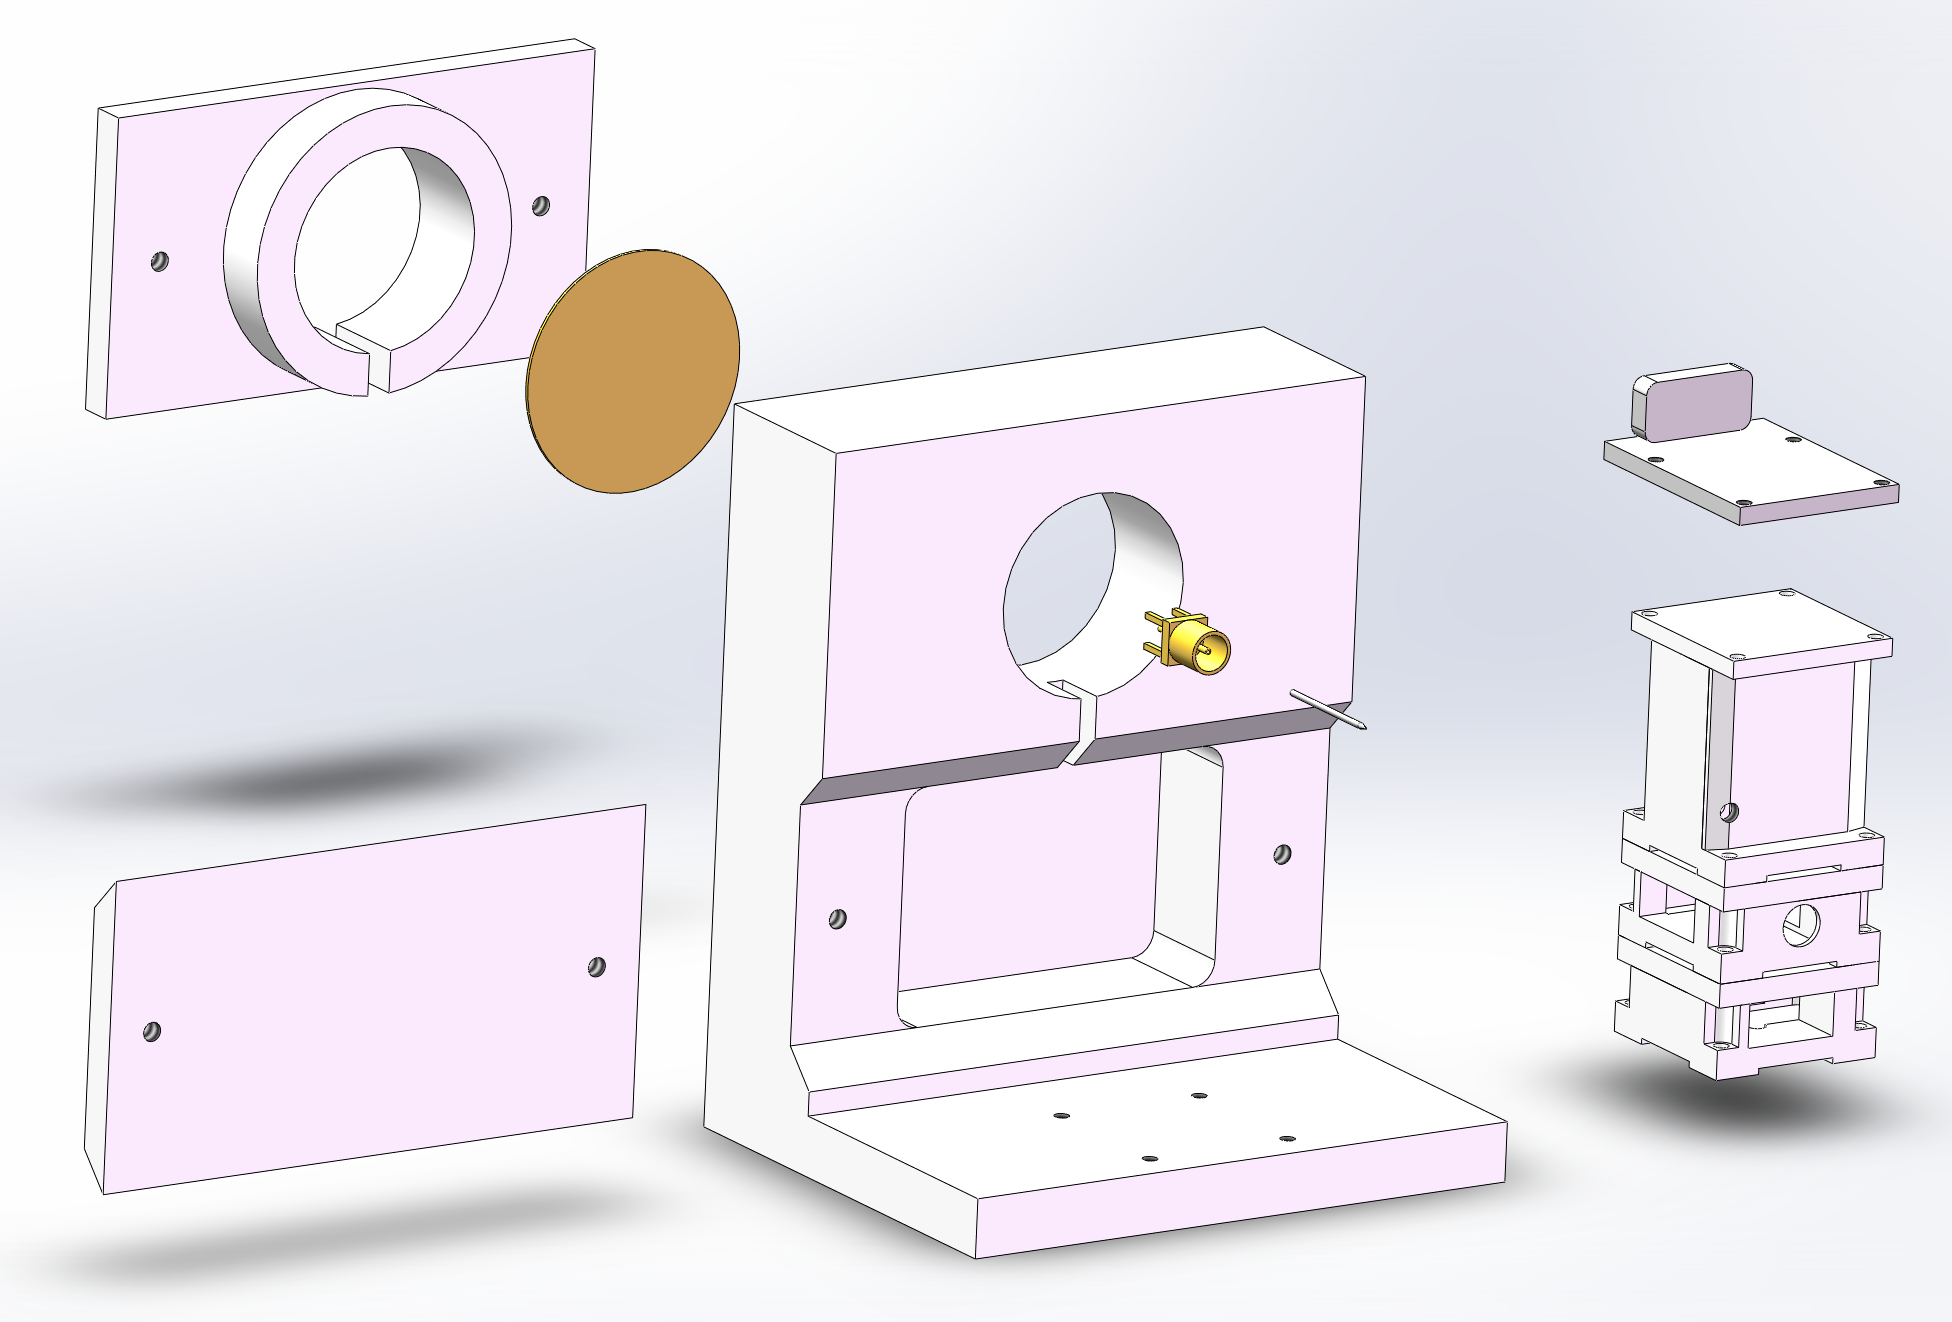
\includegraphics[width=0.9\textwidth]{fig9.png}};
				\begin{scope}[x={(image.south east)},y={(image.north west)}]
					% 建立相对坐标系
					%						\draw[help lines,xstep=.1,ystep=.1] (0,0) grid (1,1);
					%						\foreach \x in {0,1,...,9} { \node [anchor=north] at (\x/10,0) {0.\x}; }
					%						\foreach \y in {0,1,...,9} { \node [anchor=east] at (0,\y/10) {0.\y}; }
					% 作图命令
					\draw[black,ultra thick] (0.25,0.8)--(0.35,0.9)--(0.6,0.9);
					\node at(0.48,0.9)[above]{扫描头固定件};
					
					\draw[black,ultra thick,shift={(0.1,-0.1)}] (0.25,0.8)--(0.35,0.9)--(0.55,0.9);
					\node at(0.48,0.9)[above,shift={(0.1,-0.1)}]{压电陶瓷片};
					
					\draw[black,ultra thick] (0.25,0.3)--(0.15,0.4)--(0.03,0.4);
					\node at(0.09,0.4)[above]{TIA 盖板};
					
					\draw[black,ultra thick] (0.61,0.51)--(0.5,0.58)--(0.35,0.58);
					\node at(0.42,0.58)[above]{MMCX 座};
					
					\draw[black,ultra thick] (0.9,0.65)--(0.8,0.6)--(0.65,0.6);
					\node at(0.7,0.6)[above]{样品台};
					
					\draw[black,ultra thick,shift={(0,-0.35)}] (0.9,0.65)--(0.8,0.6)--(0.65,0.6);
					\node at(0.62,0.6)[above,shift={(0.1,-0.35)}]{压电滑台};
					
					\draw[black,ultra thick,shift={(-0.4,-0.5)}] (0.9,0.65)--(0.8,0.6)--(0.68,0.6);
					\node at(0.62,0.6)[above,shift={(-0.3,-0.5)}]{基座};
					
					\draw [red,rounded corners,thick](0.65,0.42)rectangle(0.71,0.5);
					\draw[black,ultra thick] (0.652,0.424)--(0.55,0.34)--(0.44,0.34);
					\node at(0.47,0.34)[above]{探针};
					
				\end{scope}
			\end{tikzpicture}\\
			\caption{机械结构示意图(正)}
		\end{subfigure}
		\vskip 1em
		\begin{subfigure}{0.8\textwidth}
			\centering
			\begin{tikzpicture}
				\node[anchor=south west,inner sep=0] (image) at (0,0) {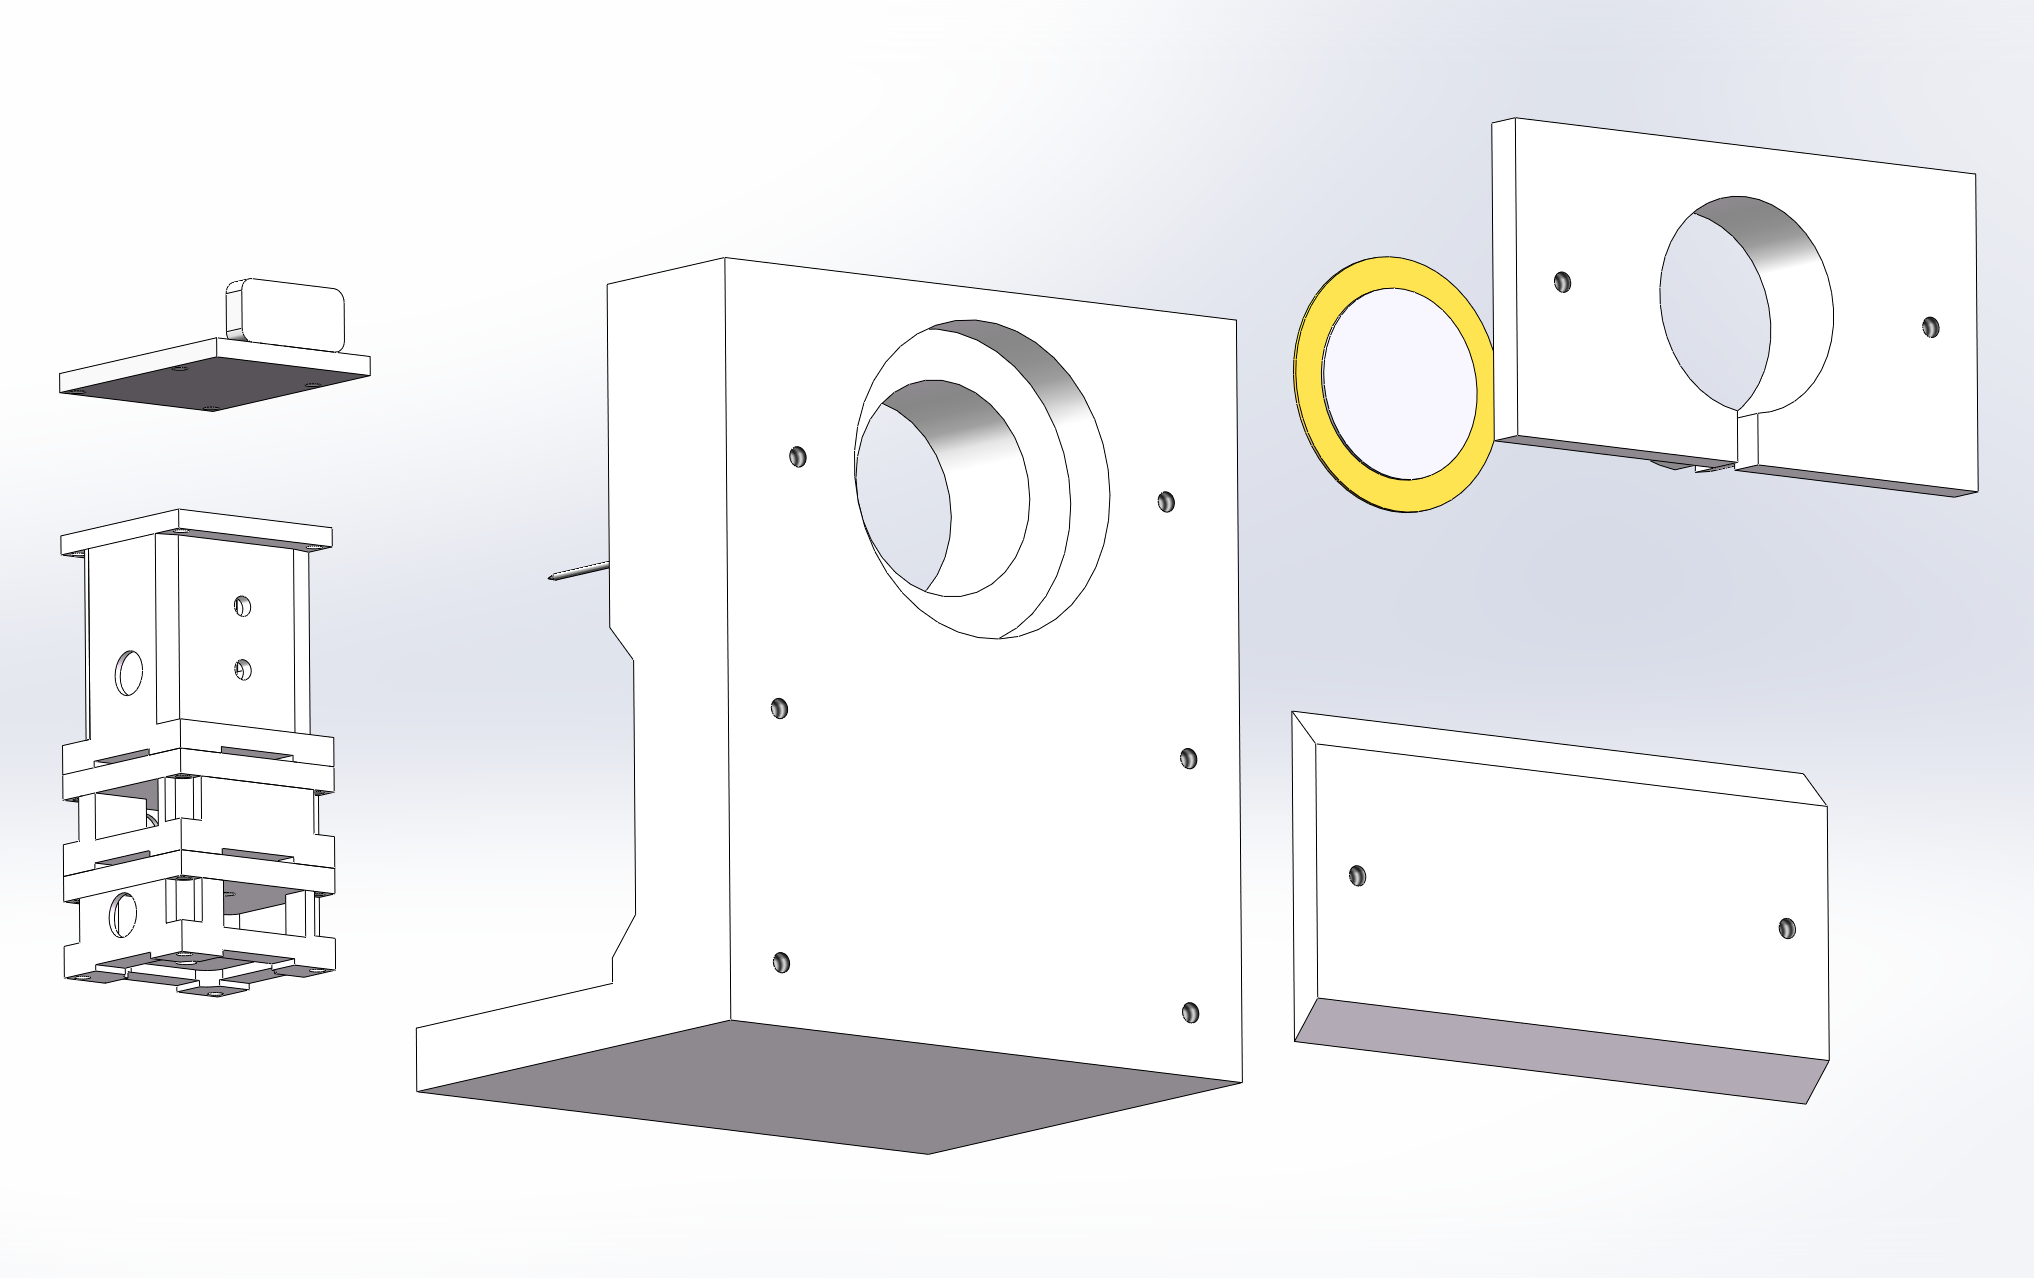
\includegraphics[width=0.9\textwidth]{fig10.png}};
				\begin{scope}[x={(image.south east)},y={(image.north west)}]
					% 建立相对坐标系
					%						\draw[help lines,xstep=.1,ystep=.1] (0,0) grid (1,1);
					%						\foreach \x in {0,1,...,9} { \node [anchor=north] at (\x/10,0) {0.\x}; }
					%						\foreach \y in {0,1,...,9} { \node [anchor=east] at (0,\y/10) {0.\y}; }
					% 作图命令
				\end{scope}
			\end{tikzpicture}
			\caption{机械结构示意图(反)}
			\label{fig18}
		\end{subfigure}
		\caption{DIY-STM 机械结构示意图}
		\label{fig7}
	\end{figure}
	\vskip 1em
	
	
	
	
	
	
	\subsubsection{扫描头的设计原理}
	本扫描头设计以 John Alexander 的“单侧变形盘状扫描头”\cite{ref13}为基础,参照 Open STM 项目\cite{ref17}进行进一步优化。如图 \ref{fig6} 所示,扫描头由四部分层叠而成,其中压电蜂鸣器是扫描头实现纳米级精细运动的关键。普通的压电蜂鸣器在施加不同电压后只能产生 Z 轴上的一维运动(如图 \ref{fig12} 所示)远不能满足 STM 探针三维移动的要求。因此我们将压电蜂鸣片上表面的银层分割为四个象限(如图 \ref{fig11} 所示),分别记为 +X、-X、+Y 和 -Y。当 +X 区域施加一个正电压,-X 区域施加一个等大的负电压时,压电蜂鸣片便会带动探针产生一个沿 X 轴方向的微小位移(如图 \ref{fig13} 所示),+Y 与 -Y 区域也是如此。由此我们便仅通过一块压电陶瓷实现了控制探针的三维移动。
	\begin{figure}[!h]
		\centering
		\begin{subfigure}{0.47\textwidth}
			\centering
			\begin{tikzpicture}
				\node[anchor=south west,inner sep=0] (image) at (0,0){
					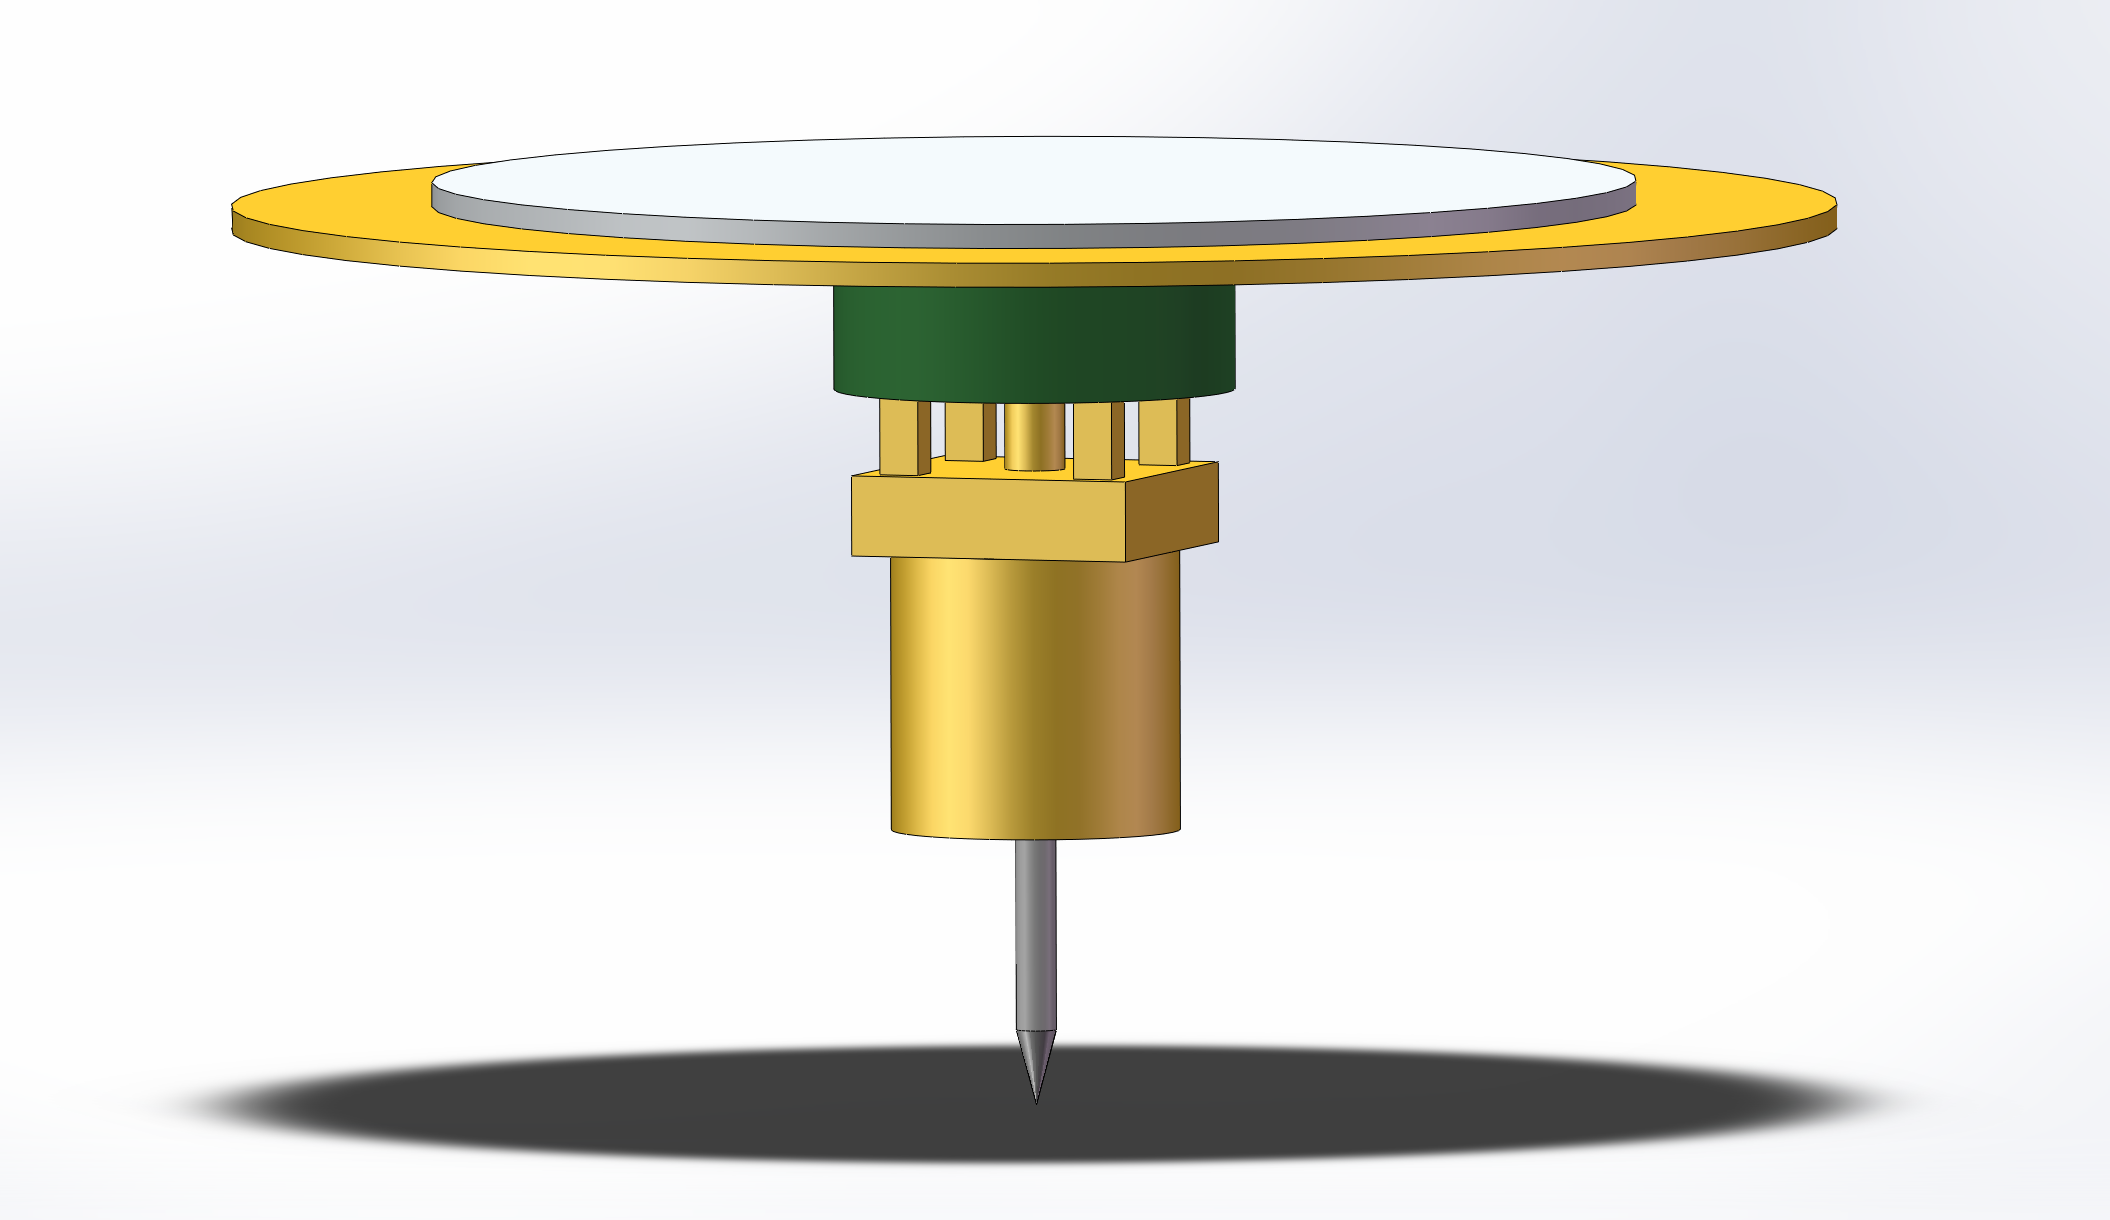
\includegraphics[width=\textwidth]{fig16.png}};
				\begin{scope}[x={(image.south east)},y={(image.north west)}]
					% 建立相对坐标系
					%							\draw[help lines,xstep=.1,ystep=.1] (0,0) grid (1,1);
					%							\foreach \x in {0,1,...,9} { \node [anchor=north] at (\x/10,0) {0.\x}; }
					%							\foreach \y in {0,1,...,9} { \node [anchor=east] at (0,\y/10) {0.\y}; }
					
					\draw[black,ultra thick] (0.2,0.8)--(0.2,0.6);
					\node at(0.2,0.6)[below]{压电蜂鸣片};
					
					\draw[black,ultra thick] (0.5,0.72)--(0.65,0.72);
					\node at(0.65,0.72)[right]{PCB 基座};
					
					\draw[black,ultra thick,shift={(0,-0.2)}] (0.5,0.72)--(0.65,0.72);
					\node at(0.65,0.72)[right,shift={(0,-0.2)}]{MMCX 座};
					
					\draw[black,ultra thick,shift={(0,-0.5)}] (0.5,0.72)--(0.65,0.72);
					\node at(0.65,0.72)[right,shift={(0,-0.5)}]{探针};
					
					\draw[->,ultra thick,red] (0.1,0.2)--(0.2,0.2);
					\node at(0.2,0.2)[right,red]{X};
					
					\draw[->,ultra thick,BlueGreen] (0.1,0.2)--(0.17,0.33);
					\node at(0.17,0.33)[right,BlueGreen]{Y};
					
					\draw[->,ultra thick,blue] (0.1,0.2)--(0.1,0.05);
					\node at(0.1,0.05)[right,blue]{Z};
					
				\end{scope}
			\end{tikzpicture}
			\caption{扫描头结构示意图}
			\label{fig6}
		\end{subfigure}
		\hfill
		\begin{subfigure}{0.45\textwidth}
			\centering
			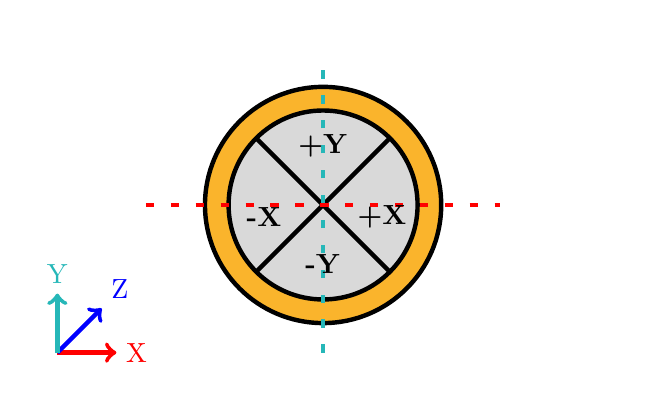
\begin{tikzpicture}[scale=0.75]
				\draw[help lines, color=white, step=1cm,ultra thin](0,0)grid(10,6);
				\draw [fill=Dandelion,ultra thick](5,3)circle(2);
				\draw [fill=gray!30,ultra thick](5,3)circle(1.6);
				
				\draw[->,ultra thick,red] (0.5,0.5)--(1.5,0.5);
				\node at(1.5,0.5)[right,red]{X};
				
				\draw[->,ultra thick,blue] (0.5,0.5)--(1.25,1.25);
				\node at(1.25,1.25)[above right,blue]{Z};
				
				\draw[->,ultra thick,BlueGreen] (0.5,0.5)--(0.5,1.5);
				\node at(0.5,1.5)[above,BlueGreen]{Y};
				
				\draw [black,ultra thick,rotate around={45:(5,3)}](3.4,3)--(6.6,3);
				\draw [black,ultra thick,rotate around={-45:(5,3)}](3.4,3)--(6.6,3);
				
				\draw [red,loosely dashed,very thick](2,3)--(8,3);
				\draw [BlueGreen,loosely dashed,very thick](5,0.5)--(5,5.5);
				
				\node at(6,2.8){\textbf{+X}};
				\node at(4,2.8){\textbf{-X}};
				\node at(5,4){\textbf{+Y}};
				\node at(5,2){\textbf{-Y}};
				
			\end{tikzpicture}
			\caption{压电蜂鸣片的分割方式}
			\label{fig11}
		\end{subfigure}
		\vskip 1em
		\begin{subfigure}{0.45\textwidth}
			\centering
			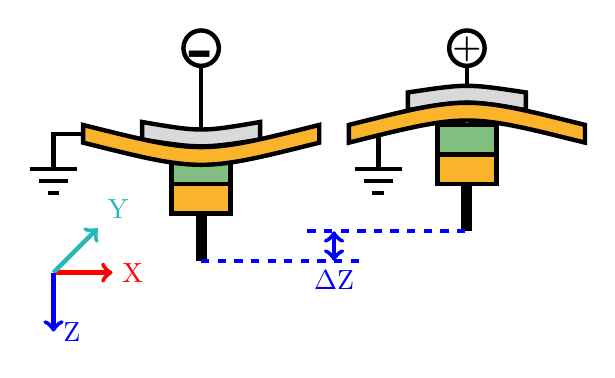
\begin{tikzpicture}[scale=0.75]
				%						\draw[help lines, color=black!30, step=1cm,ultra thin](0,0)grid(10,6);
				
				\draw[->,ultra thick,red] (0.5,1.5)--(1.5,1.5);
				\node at(1.5,1.5)[right,red]{X};
				\draw[->,ultra thick,BlueGreen] (0.5,1.5)--(1.25,2.25);
				\node at(1.25,2.25)[above right,BlueGreen]{Y};
				\draw[->,ultra thick,blue] (0.5,1.5)--(0.5,0.5);
				\node at(0.5,0.5)[right,blue]{Z};
				
				
				\draw [smooth,black,ultra thick,fill=gray!30,shift={(0,0.3)}](2,4-0.25)..controls(3,3.58)..(4,4-0.25)
				--(4,3.7-0.25)
				..controls(3,3.3)..(2,3.7-0.25)
				--cycle;
				
				\draw [fill=Dandelion,ultra thick](2.5,2.5)rectangle(3.5,3.5);
				\draw [fill=green!50!black!50,ultra thick](2.5,3)rectangle(3.5,3.5);
				\draw [black,line width=4pt](3,2.5)--(3,1.7);
				
				
				\draw [smooth,black,ultra thick,fill=Dandelion](1,4)..controls(3,3.5)..(5,4)
				--(5,3.7)
				..controls(3,3.2)..(1,3.7)
				--cycle;
				
				
				%=========================
				\draw [smooth,black,ultra thick,fill=gray!30,shift={(-4.5,0)},rotate around={180:(7.5,4)}](2,4-0.25)..controls(3,3.58)..(4,4-0.25)
				--(4,3.7-0.25)
				..controls(3,3.3)..(2,3.7-0.25)
				--cycle;
				
				
				\draw [fill=Dandelion,ultra thick,shift={(4.5,0.5)}](2.5,2.5)rectangle(3.5,3.5);
				\draw [fill=green!50!black!50,ultra thick,shift={(4.5,0.5)}](2.5,3)rectangle(3.5,3.5);
				\draw [black,line width=4pt,shift={(4.5,0.5)}](3,2.5)--(3,1.7);
				
				
				\draw [smooth,black,ultra thick,fill=Dandelion,shift={(4.5,0)}](1,4)..controls(3,4.5)..(5,4)
				--(5,3.7)
				..controls(3,4.2)..(1,3.7)
				--cycle;
				
				%=======================
				
				\draw [dashed,blue,ultra thick](3,1.7)--(5.7,1.7);
				\draw [dashed,blue,ultra thick](4.8,2.2)--(7.5,2.2);
				\draw [<->,ultra thick,blue](5.25,1.7)--(5.25,2.2);
				\node at(5.25,1.7)[below,blue]{$\Delta$Z};
				
				
				%=======================
				\draw [ultra thick,black,shift={(0,2.85)}](1,1)-|(0.5,0.4);
				\draw [ultra thick,black,shift={(0,2.85)}](0.1,0.4)--(0.9,0.4);
				\draw [ultra thick,black,shift={(0,2.85)}](0.25,0.2)--(0.75,0.2);
				\draw [ultra thick,black,shift={(0,2.85)}](0.4,0)--(0.6,0);
				
				\draw [ultra thick,black,shift={(5.5,2.85)}](0.5,1)--(0.5,0.4);
				\draw [ultra thick,black,shift={(5.5,2.85)}](0.1,0.4)--(0.9,0.4);
				\draw [ultra thick,black,shift={(5.5,2.85)}](0.25,0.2)--(0.75,0.2);
				\draw [ultra thick,black,shift={(5.5,2.85)}](0.4,0)--(0.6,0);
				
				\draw [ultra thick,black](3,3.9)--(3,5);
				\draw [ultra thick,black](3,5.3)circle(0.3);
				\node at(3,5.2){\Huge\textbf{-}};
				
				\draw [ultra thick,black](7.5,4.7)--(7.5,5);
				\draw [ultra thick,black](7.5,5.3)circle(0.3);
				\node at(7.5,5.28){\large\textbf{+}};
				
				
			\end{tikzpicture}
			\caption{普通压电蜂鸣片施加不同电压产生的形变}
			\label{fig12}
		\end{subfigure}
		\hfill
		\begin{subfigure}{0.45\textwidth}
			\centering
			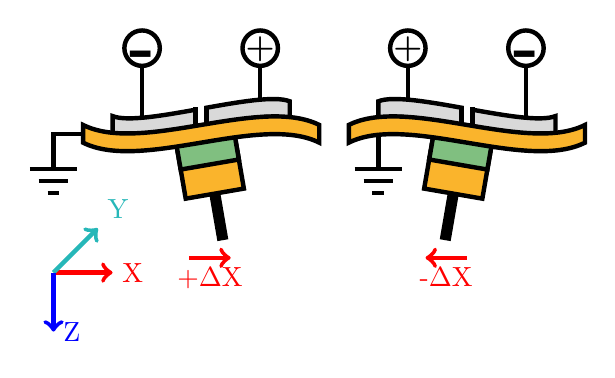
\begin{tikzpicture}[scale=0.75]
				%						\draw[help lines, color=black!30, step=1cm,ultra thin](0,0)grid(10,6);
				
				\draw[->,ultra thick,red] (0.5,1.5)--(1.5,1.5);
				\node at(1.5,1.5)[right,red]{X};
				\draw[->,ultra thick,BlueGreen] (0.5,1.5)--(1.25,2.25);
				\node at(1.25,2.25)[above right,BlueGreen]{Y};
				\draw[->,ultra thick,blue] (0.5,1.5)--(0.5,0.5);
				\node at(0.5,0.5)[right,blue]{Z};
				
				
				\draw [smooth,black,ultra thick,fill=gray!30,shift={(0,0.3)}](1.5,3.55)
				..controls(2,3.35)and(4,4)..(4.5,3.8)
				--(4.5,4.1)
				..controls(4,4.3)and(2,3.65)..(1.5,3.85)
				--cycle;
				\draw [black,line width=6pt](3,4.3)--(3,3.9);
				\draw [white,line width=2pt](3,4.4)--(3,3.9);
				
				\begin{scope}[rotate around={9.8:(3,3)},shift={(0.2,0.3)}]
					\draw [fill=Dandelion,ultra thick](2.5,2.5)rectangle(3.5,3.5);
					\draw [fill=green!50!black!50,ultra thick](2.5,3)rectangle(3.5,3.5);
					\draw [black,line width=4pt](3,2.5)--(3,1.7);
				\end{scope}
				
				
				
				\draw [smooth,black,ultra thick,fill=Dandelion](1,4)..controls(2,3.5)and(4,4.5)..(5,4)
				--(5,3.7)
				..controls(4,4.2)and(2,3.2)..(1,3.7)
				--cycle;
				
				
				%=========================
				\begin{scope}[shift={(10.5,0)},xscale=-1]
					\draw [smooth,black,ultra thick,fill=gray!30,shift={(0,0.3)}](1.5,3.55)
					..controls(2,3.35)and(4,4)..(4.5,3.8)
					--(4.5,4.1)
					..controls(4,4.3)and(2,3.65)..(1.5,3.85)
					--cycle;
					\draw [black,line width=6pt](3,4.3)--(3,3.9);
					\draw [white,line width=2pt](3,4.4)--(3,3.9);
					
					\begin{scope}[rotate around={9.8:(3,3)},shift={(0.2,0.3)}]
						\draw [fill=Dandelion,ultra thick](2.5,2.5)rectangle(3.5,3.5);
						\draw [fill=green!50!black!50,ultra thick](2.5,3)rectangle(3.5,3.5);
						\draw [black,line width=4pt](3,2.5)--(3,1.7);
					\end{scope}
					
					
					\draw [smooth,black,ultra thick,fill=Dandelion](1,4)..controls(2,3.5)and(4,4.5)..(5,4)
					--(5,3.7)
					..controls(4,4.2)and(2,3.2)..(1,3.7)
					--cycle;
					
					\draw [ultra thick,black](2,4.1)--(2,5);
					\draw [ultra thick,black](2,5.3)circle(0.3);
					\node at(2,5.2){\Huge\textbf{-}};
					
					\draw [ultra thick,black](4,4.4)--(4,5);
					\draw [ultra thick,black](4,5.3)circle(0.3);
					\node at(4,5.28){\large\textbf{+}};
					
				\end{scope}
				
				%=======================
				
				
				\draw [->,ultra thick,red](2.8,1.75)--(3.5,1.75);
				\node at(3.15,1.75)[below,red]{+$\Delta$X};
				
				\draw [->,ultra thick,red,shift={(4,0)}](3.5,1.75)--(2.8,1.75);
				\node at(3.15,1.75)[below,red,shift={(3,0)}]{-$\Delta$X};
				
				
				%=======================
				\draw [ultra thick,black,shift={(0,2.85)}](1,1)-|(0.5,0.4);
				\draw [ultra thick,black,shift={(0,2.85)}](0.1,0.4)--(0.9,0.4);
				\draw [ultra thick,black,shift={(0,2.85)}](0.25,0.2)--(0.75,0.2);
				\draw [ultra thick,black,shift={(0,2.85)}](0.4,0)--(0.6,0);
				
				\draw [ultra thick,black,shift={(5.5,2.85)}](0.5,1)--(0.5,0.4);
				\draw [ultra thick,black,shift={(5.5,2.85)}](0.1,0.4)--(0.9,0.4);
				\draw [ultra thick,black,shift={(5.5,2.85)}](0.25,0.2)--(0.75,0.2);
				\draw [ultra thick,black,shift={(5.5,2.85)}](0.4,0)--(0.6,0);
				
				\draw [ultra thick,black](2,4.1)--(2,5);
				\draw [ultra thick,black](2,5.3)circle(0.3);
				\node at(2,5.2){\Huge\textbf{-}};
				
				\draw [ultra thick,black](4,4.4)--(4,5);
				\draw [ultra thick,black](4,5.3)circle(0.3);
				\node at(4,5.28){\large\textbf{+}};
			\end{tikzpicture}
			\caption{分割后的压电蜂鸣片施加不同电压产生的形变}
			\label{fig13}
		\end{subfigure}
		\caption{扫描头原理示意图}
		\label{fig10}
	\end{figure}
	\vskip 1em
	
	
	
	
	
	
	
	\subsubsection{压电滑台的设计原理}
	惯性压电滑台是一种利用压电效应与粘滑现象制成的具有高精度、长行程的位移滑台。通过施加一
	定规律变化的电压,滑台内的压电晶体会产生相应的形变,进而通过磁铁带动滑台产生相应的移动。本系统由 Hsien-Shun Liao 等人设计的开源压电滑台\cite{ref18}进一步改进而来,其体积更小,更加适合应用于自制 STM 项目。该压电滑台可以以“高精度模式”(图 \ref{fig15})和“长行程模式”(图 \ref{fig16})两种驱动模式运行。在高精度模式下,电压以一定速率平稳变化,此时线性位移台将在磁力的和摩擦力作用下跟随压电晶体同步运动。在长行程模式下,电压先以一定速率平稳变化,此时线性位移台跟随压电晶体同步运动;随后电压迅速改变,由于惯性,线性位移台的运动将稍滞后于压电晶体,其相对于初始位置会产生一个微小位移 $\Delta s$。重复此过程积累位移即可实现长行程的精确移动。
	\begin{figure}[htbp]
		\centering
		\begin{subfigure}{0.49\linewidth}
			\centering
			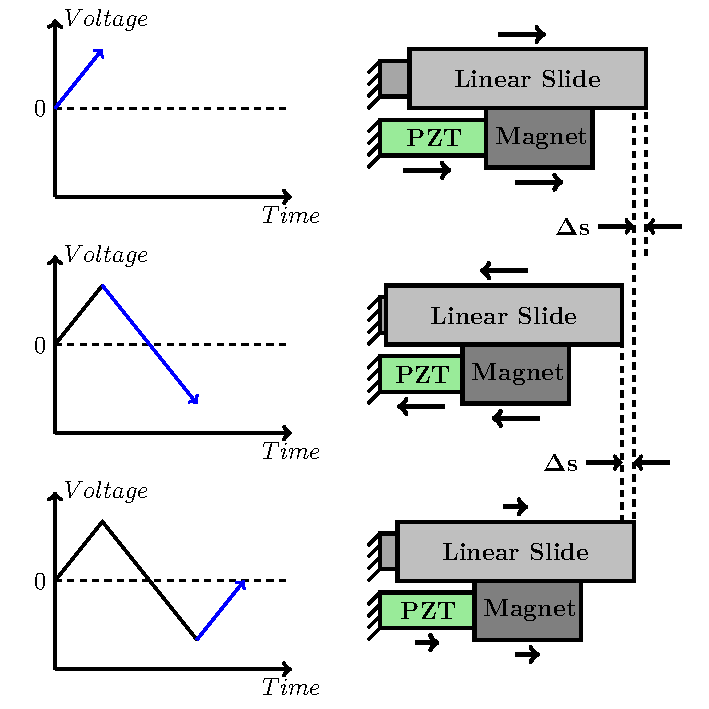
\includegraphics[width=\textwidth]{tex/fig1/fig1.pdf}
			\caption{高精度模式}
			\label{fig15}
		\end{subfigure}
		\hfill
		\begin{subfigure}{0.49\linewidth}
			\centering
			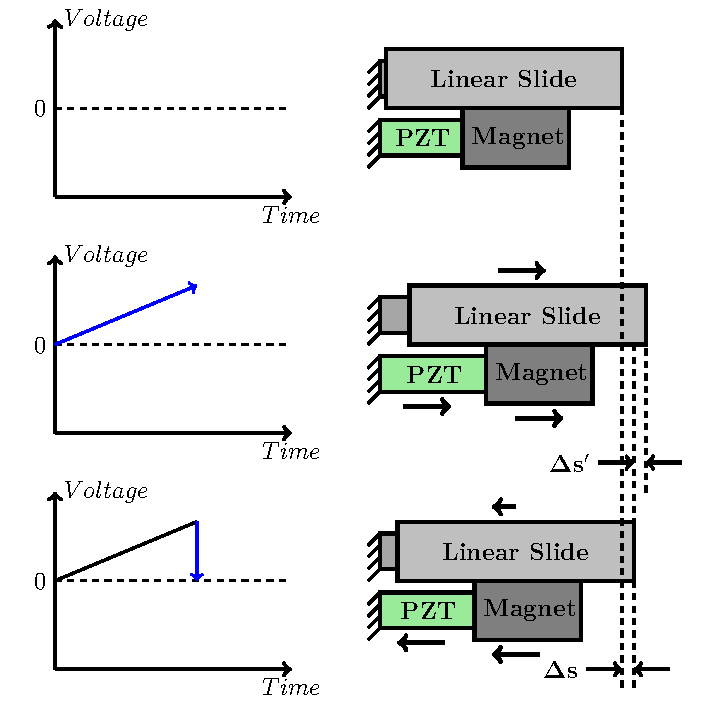
\includegraphics[width=\textwidth]{tex/fig2/fig2.pdf}
			\caption{长行程模式}
			\label{fig16}
		\end{subfigure}
		\caption{压电滑台原理示意图}
		\label{fig14}
	\end{figure}
	\vskip 1em
	
	
	
	\subsubsection{减震系统的设计原理}
	本设计方案采用简单的悬挂减震系统为 STM 主体滤除高频振动带来的影响。同时我们分别在减震平台下方和底座上安装铝板与磁铁以增加电磁阻尼,使系统能够更快地衰减高频振动。其设计原理图如图 \ref{fig17} 所示。
	
	\begin{figure}[htbp]
		\centering
		\begin{tikzpicture}
			%					\draw[help lines, color=black, step=1cm,ultra thin](0,0)grid(10,6);
			\begin{scope}[shift={(3,0)}]
				\draw [black!30,line width=5pt](2,0)--(2,6);
				\draw [black,line width=10pt](0,0)--(4,0);
				\draw [black,line width=10pt](0,5)--(4,5);
				\draw [black,line width=5pt](0.5,0)--(0.5,6);
				\draw [black,line width=5pt](3.5,0)--(3.5,6);
				\draw [black,line width=8pt](0.5,5.3)--(0.5,6);
				\draw [black,line width=8pt](2,5.3)--(2,6);
				\draw [black,line width=8pt](3.5,5.3)--(3.5,6);
				
				\draw [black,line width=10pt](1,1.5)--(3,1.5);
				\draw [blue,line width=8pt](1,0.3)--(3,0.3);
				\draw [gray,line width=7pt](1,1.3)--(3,1.3);
				
				\draw [dashed,very thick,black](1,1.7)--(0.6,5);
				\draw [dashed,very thick,black](2,1.7)--(2,5);
				\draw [dashed,very thick,black](3,1.7)--(3.4,5);
			\end{scope}
			
			\draw [very thick, black](2,0.3)--(4,0.3);
			\node at(2,0.4)[left]{强磁铁};
			
			\draw [very thick, black](2,1)--(3,1)--(4,1.3);
			\node at(2,1)[left]{铝板};
			
			\draw [very thick, black](2,2)--(3,2)--(4,1.5);
			\node at(2,2)[left]{平台};
			
			\draw [very thick, black](2,3)--(3.8,3);
			\node at(2,3)[left]{弹簧};
			
			\draw [very thick, black](6.7,0)--(7.3,0.5)--(8,0.5);
			\node at(8,0.5)[right]{底座};
			
			\draw [very thick, black](6.5,3)--(8,3);
			\node at(8,3)[right]{螺杆};
			
			\draw [very thick, black](6.5,5.5)--(8,5.5);
			\node at(8,5.5)[right]{螺帽};
			
		\end{tikzpicture}
		\caption{减震系统原理示意图}
		\label{fig17}
	\end{figure}
	\vskip 1em
	
	
	
	
	
	
	\subsection{电子电路}
	电子电路部分主要完成隧穿电流的采集与放大、将数字信号转化为模拟信号以驱动压电滑台和扫描头、执行基本控制指令以及与实现上位机之间的通信等任务。详细电路设计原理图及 PCB 图纸见附录 A。
	\begin{enumerate}
		\item \textbf{电源板(Power\_Board)}\par
		\qquad 电源板通过 USB-A 获得 5V 供电,经由 DC-DC 芯片(ADP5070)产生 $\pm$15V 电压对外输出,其中 +15V 电压经由 LDO(7812 / 7912 / 7805 / LD1117)转化为低波纹、低噪声的 $\pm$12V、5V 和 3.3V 电压输出。
		
		\item \textbf{压电滑台驱动板(Motor\_Board)}\par
		\qquad 压电滑台驱动板通过排线与 ADC \& MCU 板相连。其上的三颗 16-bit DAC(AD5761)分别将接收到的数字信号转化为 X、Y、Z 三个通道的电压输出,用于驱动压电滑台。
		
		\item \textbf{扫描头驱动板(Controller\_Board)}\par
		\qquad 扫描头驱动板同样通过排线与 ADC \& MCU 板相连。其上的四颗 16-bit DAC(AD5761)分别将接收到的数字信号转化为 X、Y、Z 以及 BIAS 四个通道的电压,其中 BIAS 直接作为偏置电压输出,其余三个电压经过运算放大器(OPA2227)运算后输出 Z+X、Z-X、Z+Y 和 Z-Y 四个电压,分别对应压电陶瓷片 +X、-X、+Y、-Y 四个区域。
		
		\item \textbf{ADC \& MCU 板(ADC\_And\_MCU\_Board)}\par
		\qquad 该电路板将接收前置放大器放大后的电流信号,利用其上的 16-bit ADC(ADS-8685)将模拟信号转化为数字信号并将信息转递给 MCU(STM32F03C8T6)。MCU 负责驱动控制 DAC 和 ADC,控制 OLED 的显示内容以及接收、传递数据的任务。MCU 通过两个硬件 SPI 控制 DAC 和 ADC,使用软件模拟 I$^\text{2}$C 控制 OLED 的显示,通过 USART 与电脑进行通信。
		
		\item \textbf{转接板(Base\_Connector\_Board)}\par
		\qquad 承担电路板与 STM 本体以及前置放大器之间的线路转接工作。
		
		\item \textbf{前置放大器(TIA\_Board)}\par
		\qquad 前置放大器采用了跨阻放大器(TIA)方案,它由一个精密运放(OPA627)和一个反馈电阻组成。当反馈电阻为 100M$\Omega$ 时,其可以将 1nA 的输入电流放大为 0.1V 电压在输出端输出。
		
	\end{enumerate}
	
	
	
	
	
	
	\subsection{控制软件}
	控制软件的开发应包括以下功能:
	\begin{enumerate}
		\item \textbf{用户界面}:设计直观、简洁的用户界面,使用户能够轻松控制 STM 并监控状态。
		\item \textbf{数据采集}:实现数据采集功能,包括隧穿电流的实时记录和存储。
		\item \textbf{反馈系统}:利用 PID 控制原理对系统进行反馈控制。
		\item \textbf{命令传递}:实现命令下达功能,传递用户操作指令。
		\item \textbf{图像处理}:开发图像重建算法,将隧穿电流信号转换为样品表面的三维图像。
	\end{enumerate}
	
	
	\subsubsection{用户界面设计}
	用户界面采用 PyQt 设计工具 Qt Designer 开发,其包含串口选择与连接、数据可视化、硬件控制、系统状态监测等一系列功能。GUI 主界面分为四个大区域:结果显示区、调试信息、硬件控制区以及状态监视区(图 \ref{fig19})。结果显示区可以绘制偏压-隧穿电流曲线、时间-隧穿电流曲线等曲线测试图,也可以绘制由隧穿电流数据处理后转化为的样品表面二维图像。调试信息区负责显示程序运行的运行信息,便于操作与调试。硬件控制区负责设置 DAC 寄存器的值以控制压电滑台、扫描头以及偏转电压,可选择控制对象与控制方式。状态监视区负责显示系统运行状态和任务执行进度,便于随时检查设备与软件运行情况。
	
	\begin{figure}[!h]
		\centering
		\begin{tikzpicture}
			begin{tikzpicture}
			\node[anchor=south west,inner sep=0] (image) at (0,0) {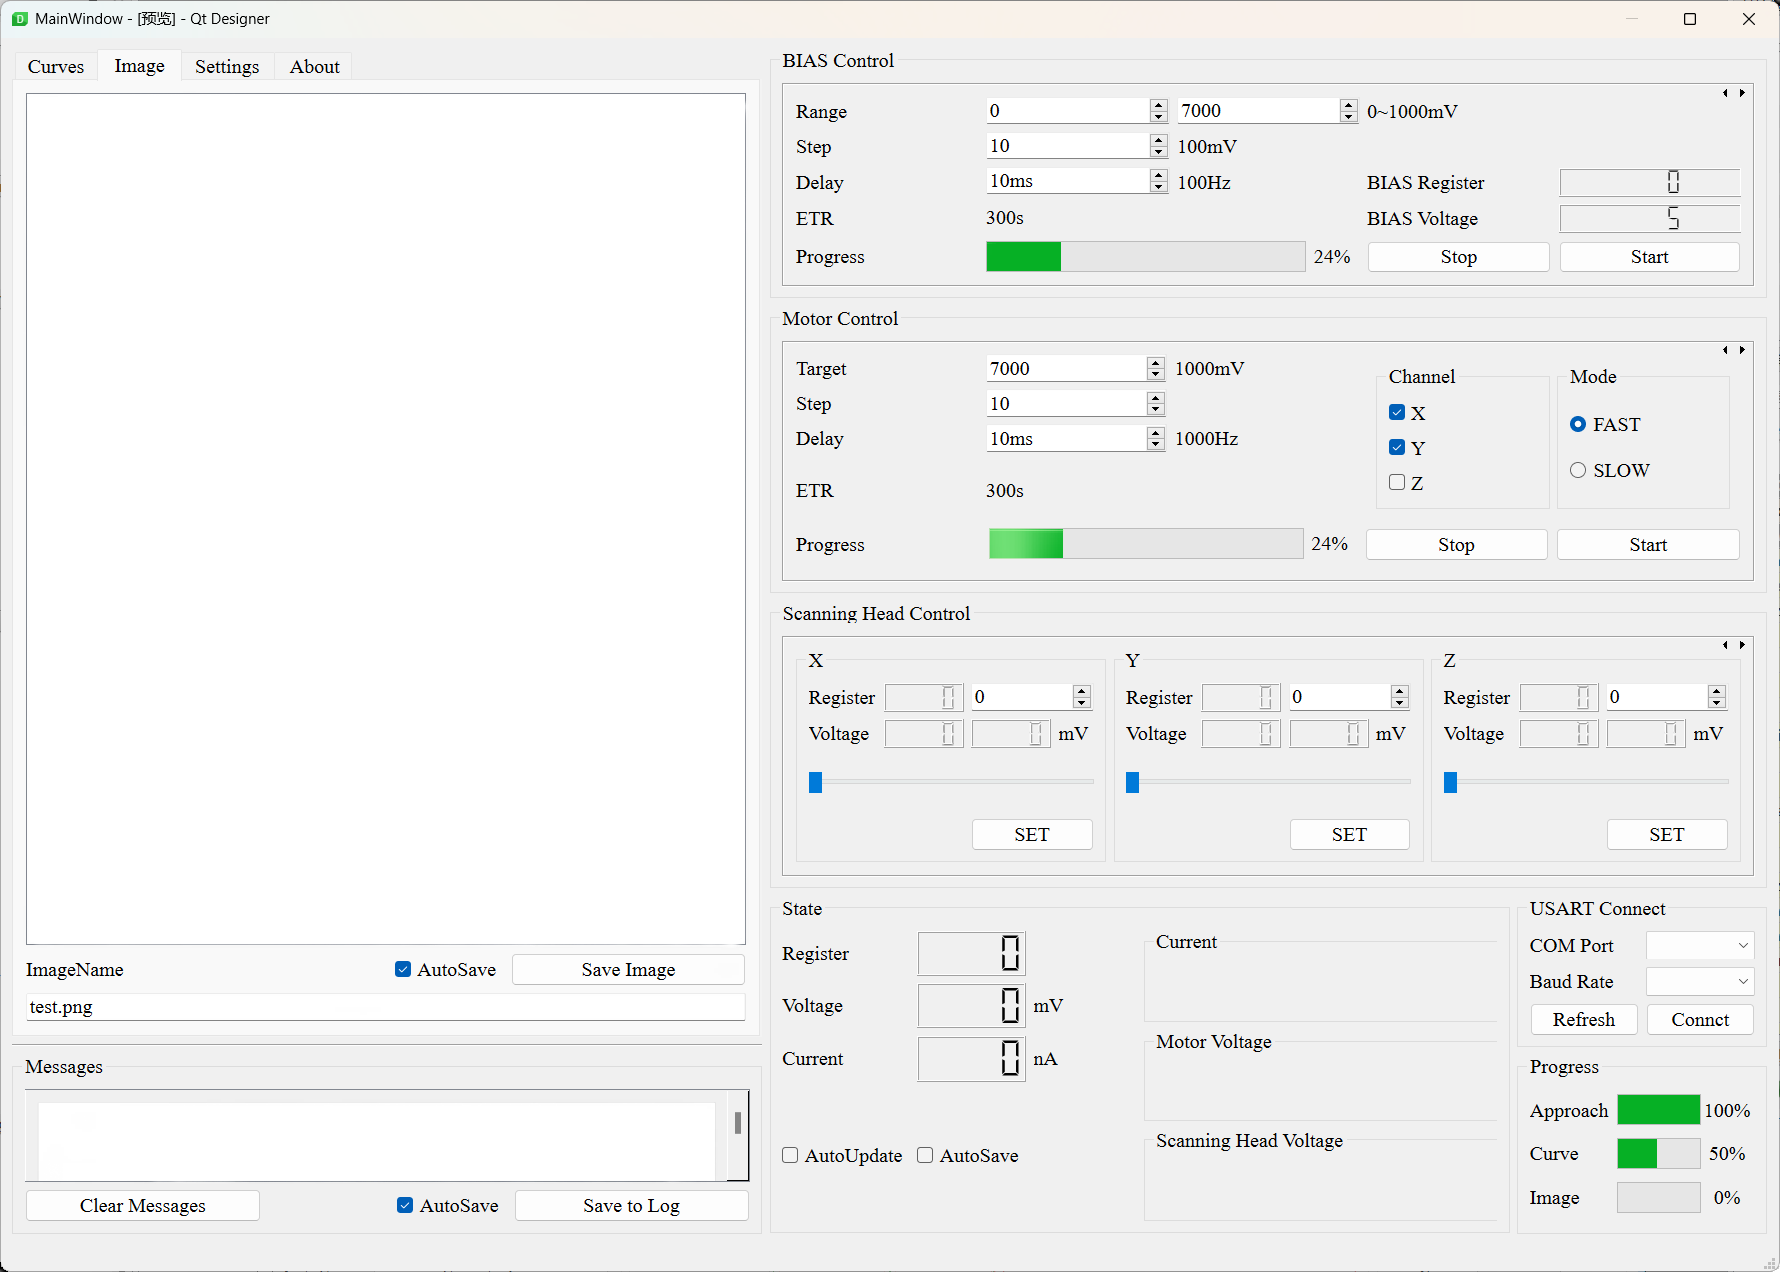
\includegraphics[width=0.8\textwidth]{GUI.png}};
			\begin{scope}[x={(image.south east)},y={(image.north west)}]
				%					 	建立相对坐标系
				%						\draw[help lines,xstep=.1,ystep=.1] (0,0) grid (1,1);
				%						\foreach \x in {0,1,...,9} { \node [anchor=north] at (\x/10,0) {0.\x}; }
				%						\foreach \y in {0,1,...,9} { \node [anchor=east] at (0,\y/10) {0.\y}; }
				%					 	作图命令
				\draw [ultra thick](0.005,0.21)rectangle(0.42,0.95);
				\node at(0.21,0.58){\bf 结果显示区};
				
				\draw [ultra thick](0.005,0.01)rectangle(0.42,0.18);
				\node at(0.21,0.1){\bf 调试信息};
				
				\draw [ultra thick](0.45,0.31)rectangle(0.98,0.95);
				\node at(0.72,0.61){\bf 硬件控制区};
				
				\draw [ultra thick](0.45,0.01)rectangle(0.98,0.28);
				\node at(0.72,0.15){\bf 状态监视区};
				
			\end{scope}
		\end{tikzpicture}
		\caption{控制软件 GUI 界面}
		\label{fig19}
	\end{figure}
	
	
	
	\subsubsection{PID 反馈控制}		
	PID(比例-积分-微分)反馈控制系统是 STM 中至关重要的组成部分,它负责维持探针与样品表面之间的恒定距离(恒定电流),从而实现对样品表面的扫描。PID 控制器是一种线性控制器,它将给定值(r(t))与实际输出值(c(t))的偏差(e(t))的比例(P)、积分(I)、微分(D)通过线性组合构成控制量(u(t)),依此对控制对象进行控制\cite{ref20}。PID 控制器的工作原理基于以下三个部分:
	\begin{itemize}
		\item \textbf{比例(P)}:控制器输出与当前误差成比例。比例控制有利于减少当前误差,但可能存在稳态误差。
		
		\item \textbf{积分(I)}:控制器输出与误差随时间累积的总和(积分)成比例。积分控制可以消除稳态误差,但可能导致系统产生过冲和振荡。
		
		\item \textbf{微分(D)}:控制器输出与误差随时间变化率成比例。微分控制可以帮助预测系统未来行为,减少过冲与震荡并提高系统稳定性。
	\end{itemize}
	
	\begin{figure}[!h]
		\centering
		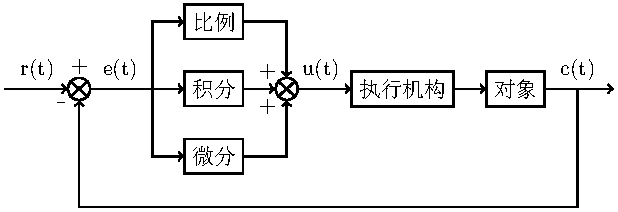
\includegraphics[width=0.8\textwidth]{/tex/fig3/fig3.pdf}
		\caption{PID 控制系统原理框图}
	\end{figure}
	
	
	在 STM 系统中,PID 控制器需要根据实际的隧穿电流信号来调整探针的 Z 轴位置。例如在恒流模式中,如果隧穿电流增大,表明探针可能离样品表面过近,PID 控制器将指令压电陶瓷扫描器使探针上升,以保持恒定的隧道电流。相反,如果隧穿电流减小,表明探针可能离样品表面过远,控制器将指令探针下降。
	
	为了实现有效的PID控制,需要对PID参数(即比例、积分、微分系数)进行精确的调整。这通常通过试错法或使用更高级的参数优化算法来完成。在本项目中,可以通过软件界面来调整这些参数,并实时观察控制效果,直至找到最佳的 PID 参数设置。
	
	
	
	
	\subsubsection{数据处理}
	数据处理是 STM 系统中不可或缺的一部分,它负责将探针扫描得到的隧穿电流信号转换为有关样品表面的详细信息。可以利用 Python 的 Scipy 库中的 curve\_fit 函数对电流数据集进行函数拟合,再借助 Numpy 库与 Matplotlib 库将曲线输出至图像。此外还可以利用 Matplotlib 库实现从散点数据到样品表面二维或三维图像的转化,从而获得样品表面的形貌特征。
	
	\begin{figure}[!h]
		\centering
		\begin{subfigure}{0.3\textwidth}
			\centering
			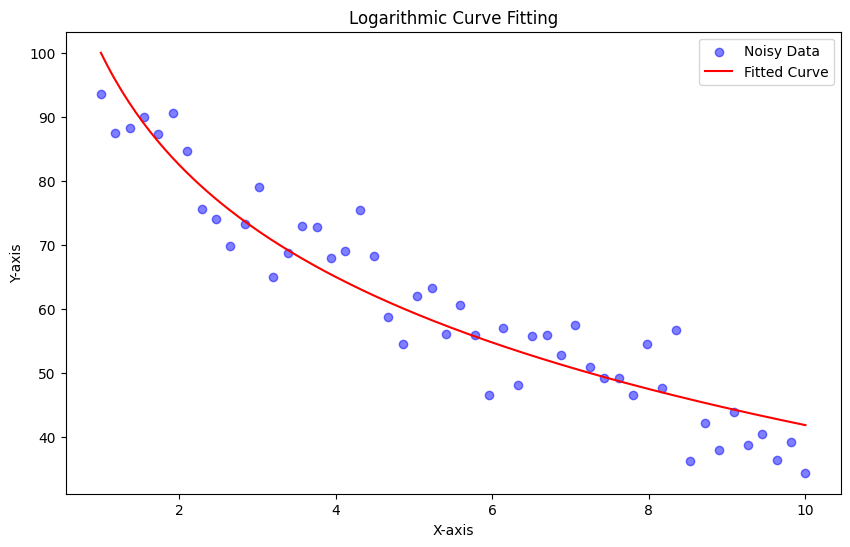
\includegraphics[width=\textwidth]{5.png}
			\caption{曲线拟合}
		\end{subfigure}
		\hfill
		\begin{subfigure}{0.3\textwidth}
			\centering
			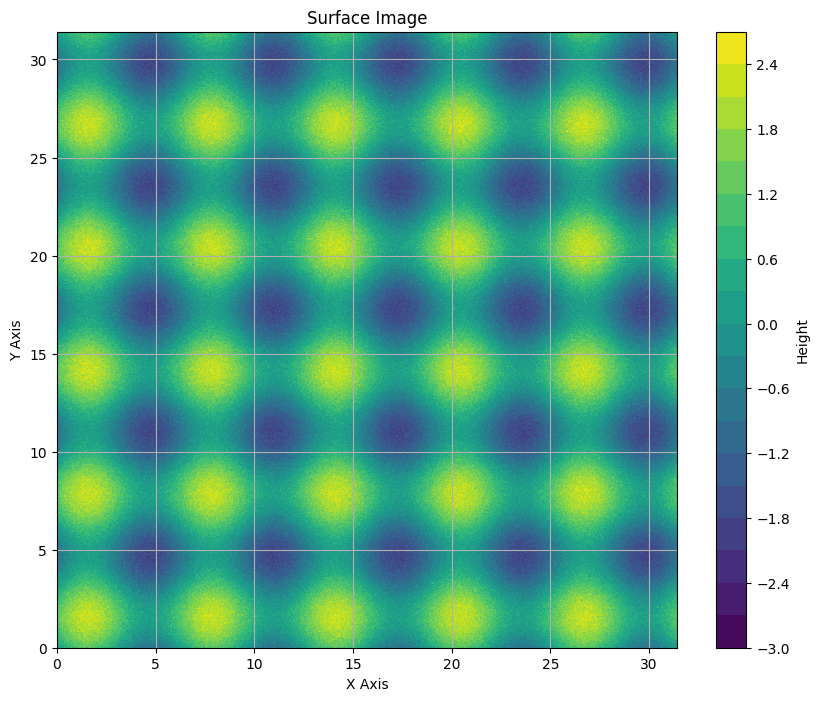
\includegraphics[width=\textwidth]{3.png}
			\caption{二维图像重建}
		\end{subfigure}
		\hfill
		\begin{subfigure}{0.3\textwidth}
			\centering
			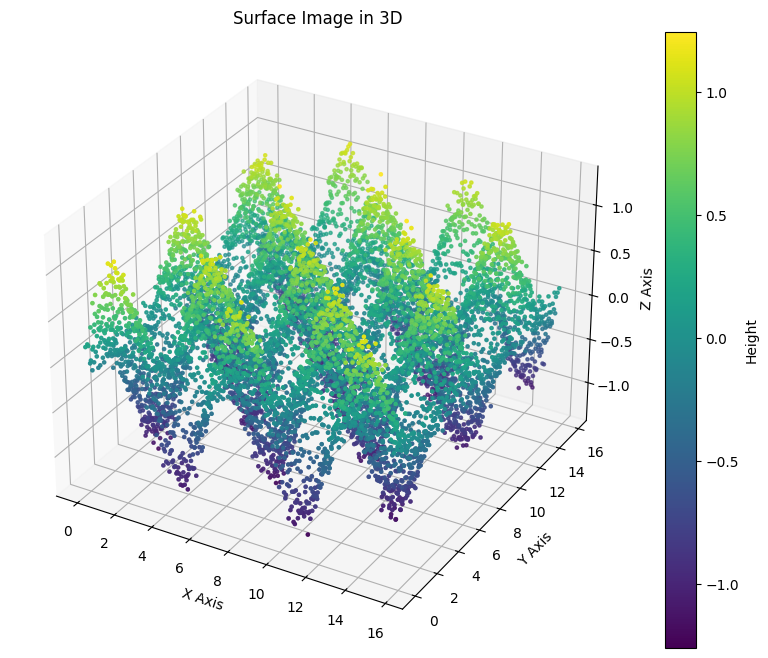
\includegraphics[width=\textwidth]{4.png}
			\caption{三维图像重建}
		\end{subfigure}
		\caption{示例代码输出结果}
		\begin{minipage}{0.95\linewidth}
			附注:示例代码见附录 B。代码与结果仅作算法展示与功能示范,使用数据集为模拟生成数据。
		\end{minipage}
	\end{figure}
	\vskip 1em
	
	
	
	
	
	
	\subsection{STM 的组装与操作}
	\subsubsection{组装扫描头}
	扫描头由四部分组成:探针、MMCX 座、PCB 基座以及盘状压电陶瓷。
	\begin{itemize}
		\item \textbf{探针}:探针使用直径 0.5 mm 的钨丝直接裁剪制成。将获得的针尖安装在 MMCX 座内孔中并启动 STM 进行测试。倘若扫描精度不理想,则再次裁剪并重复测试,直至获得足够尖锐的针尖。
		
		\item \textbf{MMCX 座}:使用 Kinghelm 公司生产的 KH-MMCX-KE-STM,将其焊接在 PCB 基座上。
		
		\item \textbf{PCB 基座}:使用漆包线将 PCB 基座上的两个焊盘分别连接在 TIA 板上的 in 焊盘以及 GND 焊盘上。使用环氧树脂胶粘剂(Ergo 5400)将其固定于压电蜂鸣片的铜层中心。
		
		\item \textbf{盘状压电陶瓷}:使用市面上常见的压电蜂鸣片作为盘状压电陶瓷。使用刻刀将压电蜂鸣片上的银层划分为四个部分,并用低温锡膏与漆包线将其与转接板的 Z+X、Z-X、Z+Y、Z-Y 四个接点相连。
		
	\end{itemize}
	
	
	
	
	
	
	
	\subsubsection{组装压电滑台}
	压电滑台结构件以铝合金-6061 作为材料,采用数控加工方式制作。压电陶瓷的位移量需较大一些,故选取 2007 年 NEC(Tokin)公司生产的堆叠压电陶瓷。线性位移台选择 IKO Nippon Thompson 公司制造的 BSP7-15SL 精密直线导轨。使用 3 个 DL-MMCX-KE\footnote{可替换为 KH-MMCX-KE-STM} 作为外接接口。磁铁选择 3$\times$3$\times$2 钕铁硼磁铁。备齐材料后,按照图 \ref{fig20} 所示步骤依次组装好两个水平滑台和一个垂直滑台,使用 8 颗 M1.6 紧固螺丝将三个滑台层叠(自下而上顺序:水平-水平-垂直)固定在一起,注意两个水平压电滑台朝向应垂直,各压电滑台接口应朝外。
	
	\begin{figure}[htbp]
		\centering
		\begin{subfigure}{0.45\textwidth}
			\centering
			\begin{tikzpicture}[scale=0.75]
				\node[anchor=south west,inner sep=0] (image) at (0,0){
					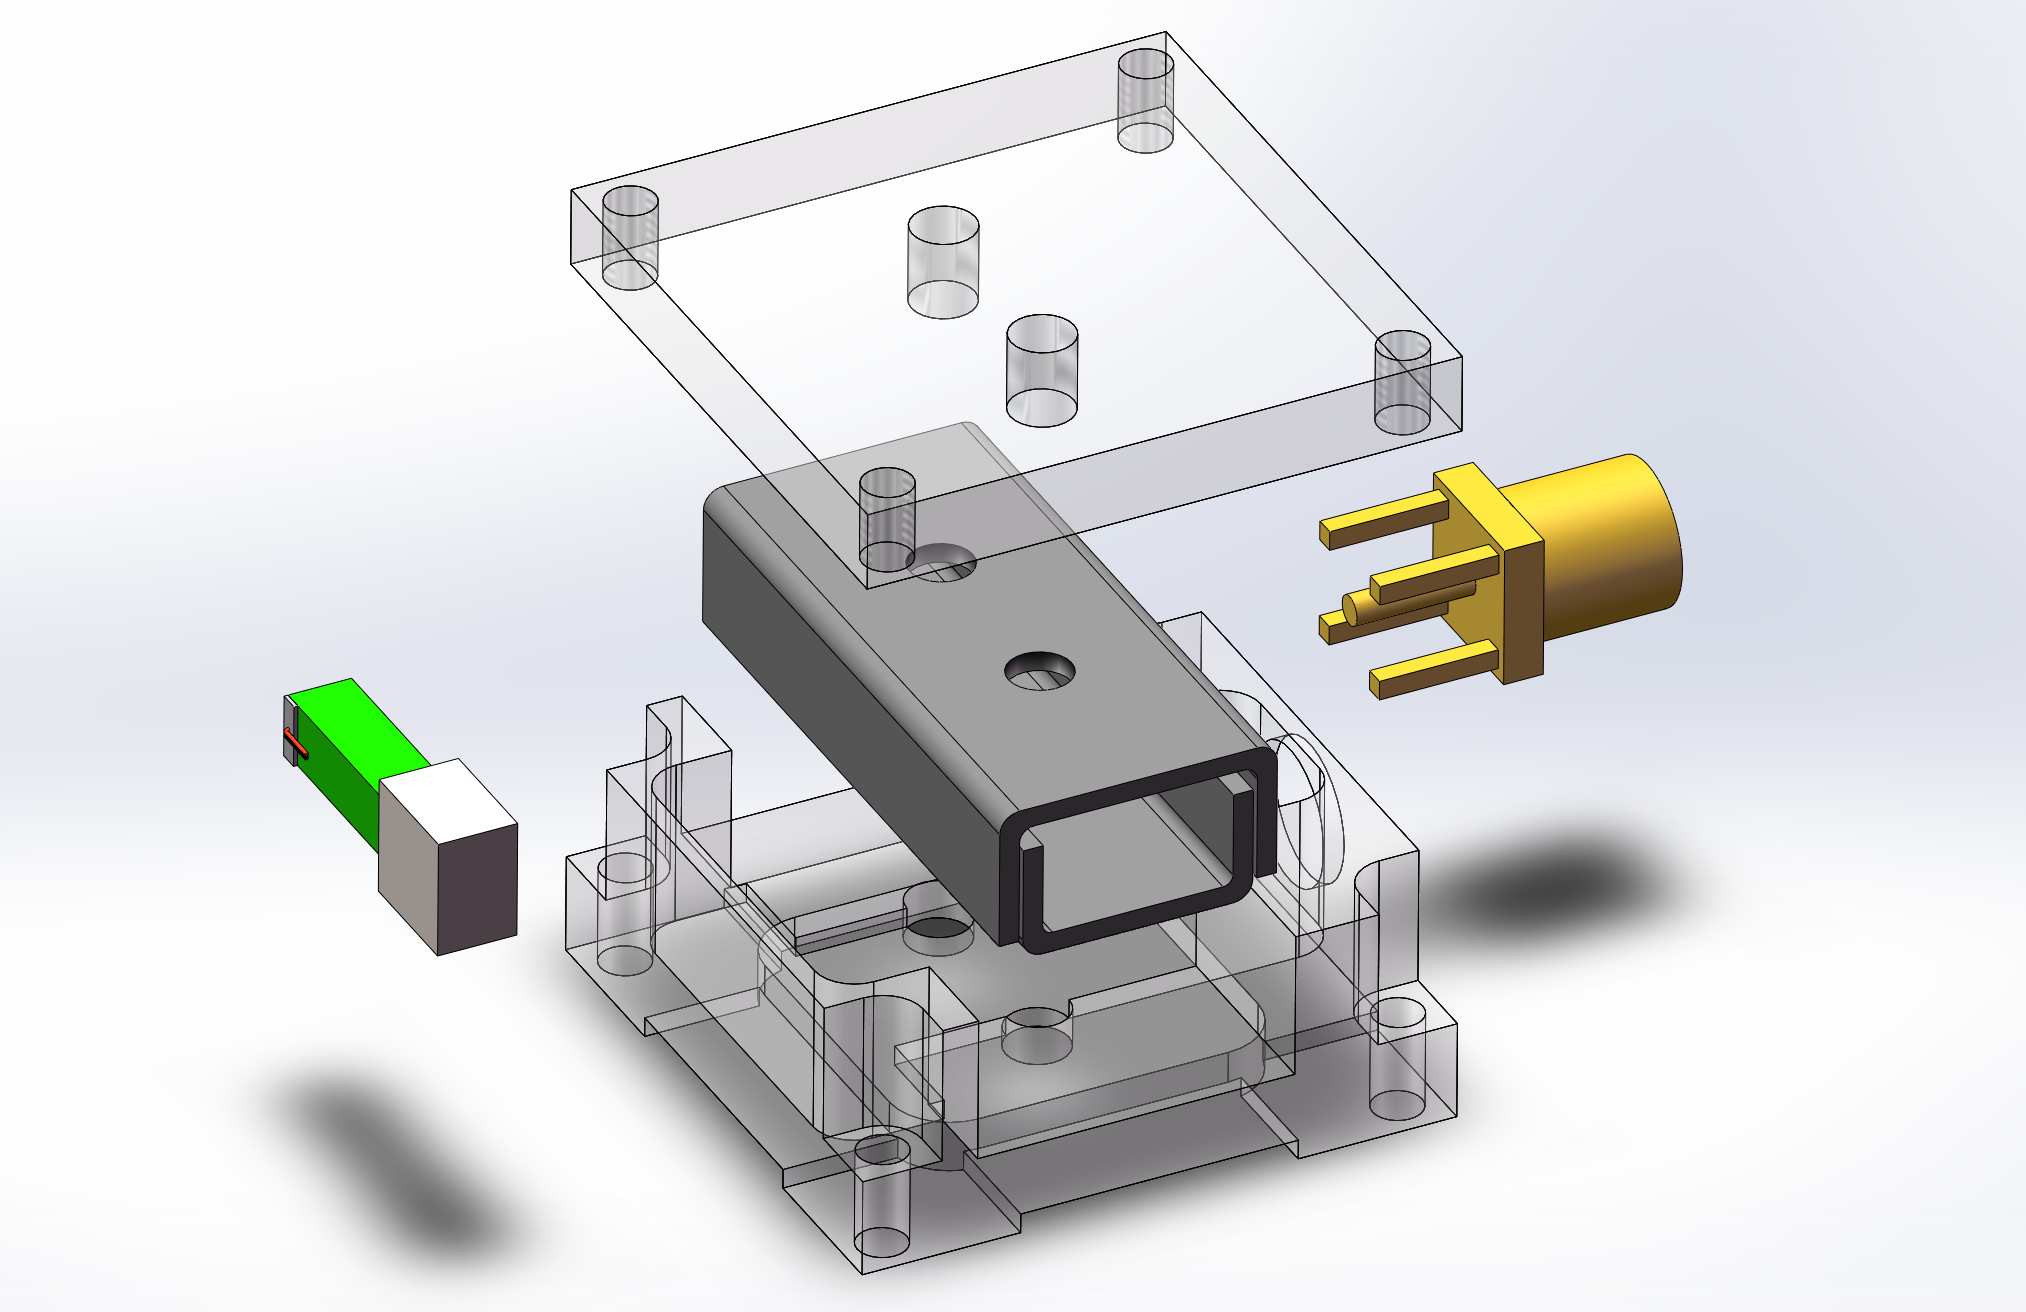
\includegraphics[width=\textwidth]{fig17.png}};
				\begin{scope}[x={(image.south east)},y={(image.north west)}]
					% 建立相对坐标系
					%							\draw[help lines,xstep=.1,ystep=.1] (0,0) grid (1,1);
					%							\foreach \x in {0,1,...,9} { \node [anchor=north] at (\x/10,0) {0.\x}; }
					%							\foreach \y in {0,1,...,9} { \node [anchor=east] at (0,\y/10) {0.\y}; }
					
					\draw [ultra thick](0.8,0.6)--(0.82,0.8);
					\node at(0.82,0.8)[above]{1:MMCX 座};
					
					\draw [ultra thick](0.18,0.41)--(0.1,0.2);
					\node at(0.1,0.2)[below]{2:压电晶体};
					\draw [ultra thick](0.22,0.3)--(0.3,0.1);
					\node at(0.3,0.1)[below]{2:磁铁};
					
					\draw [ultra thick](0.36,0.6)--(0.3,0.6);
					\node at(0.3,0.6)[left]{3:直线导轨};
					
					\draw [ultra thick](0.3,0.8)--(0.2,0.8);
					\node at(0.2,0.8)[left]{4:平台};
					
					\draw [ultra thick](0.7,0.18)--(0.8,0.1);
					\node at(0.8,0.1)[right]{底座};
					
					\draw [ultra thick](0.47,0.82)--(0.495,0.9);
					\draw [ultra thick](0.51,0.72)--(0.505,0.9);
					\node at(0.5,0.9)[above]{5:4$\times$M2};
					
				\end{scope}
			\end{tikzpicture}
			\caption{组装过程(水平)}
		\end{subfigure}
		\hfill
		\begin{subfigure}{0.45\textwidth}
			\centering
			\begin{tikzpicture}[scale=0.75]
				\node[anchor=south west,inner sep=0] (image) at (0,0){
					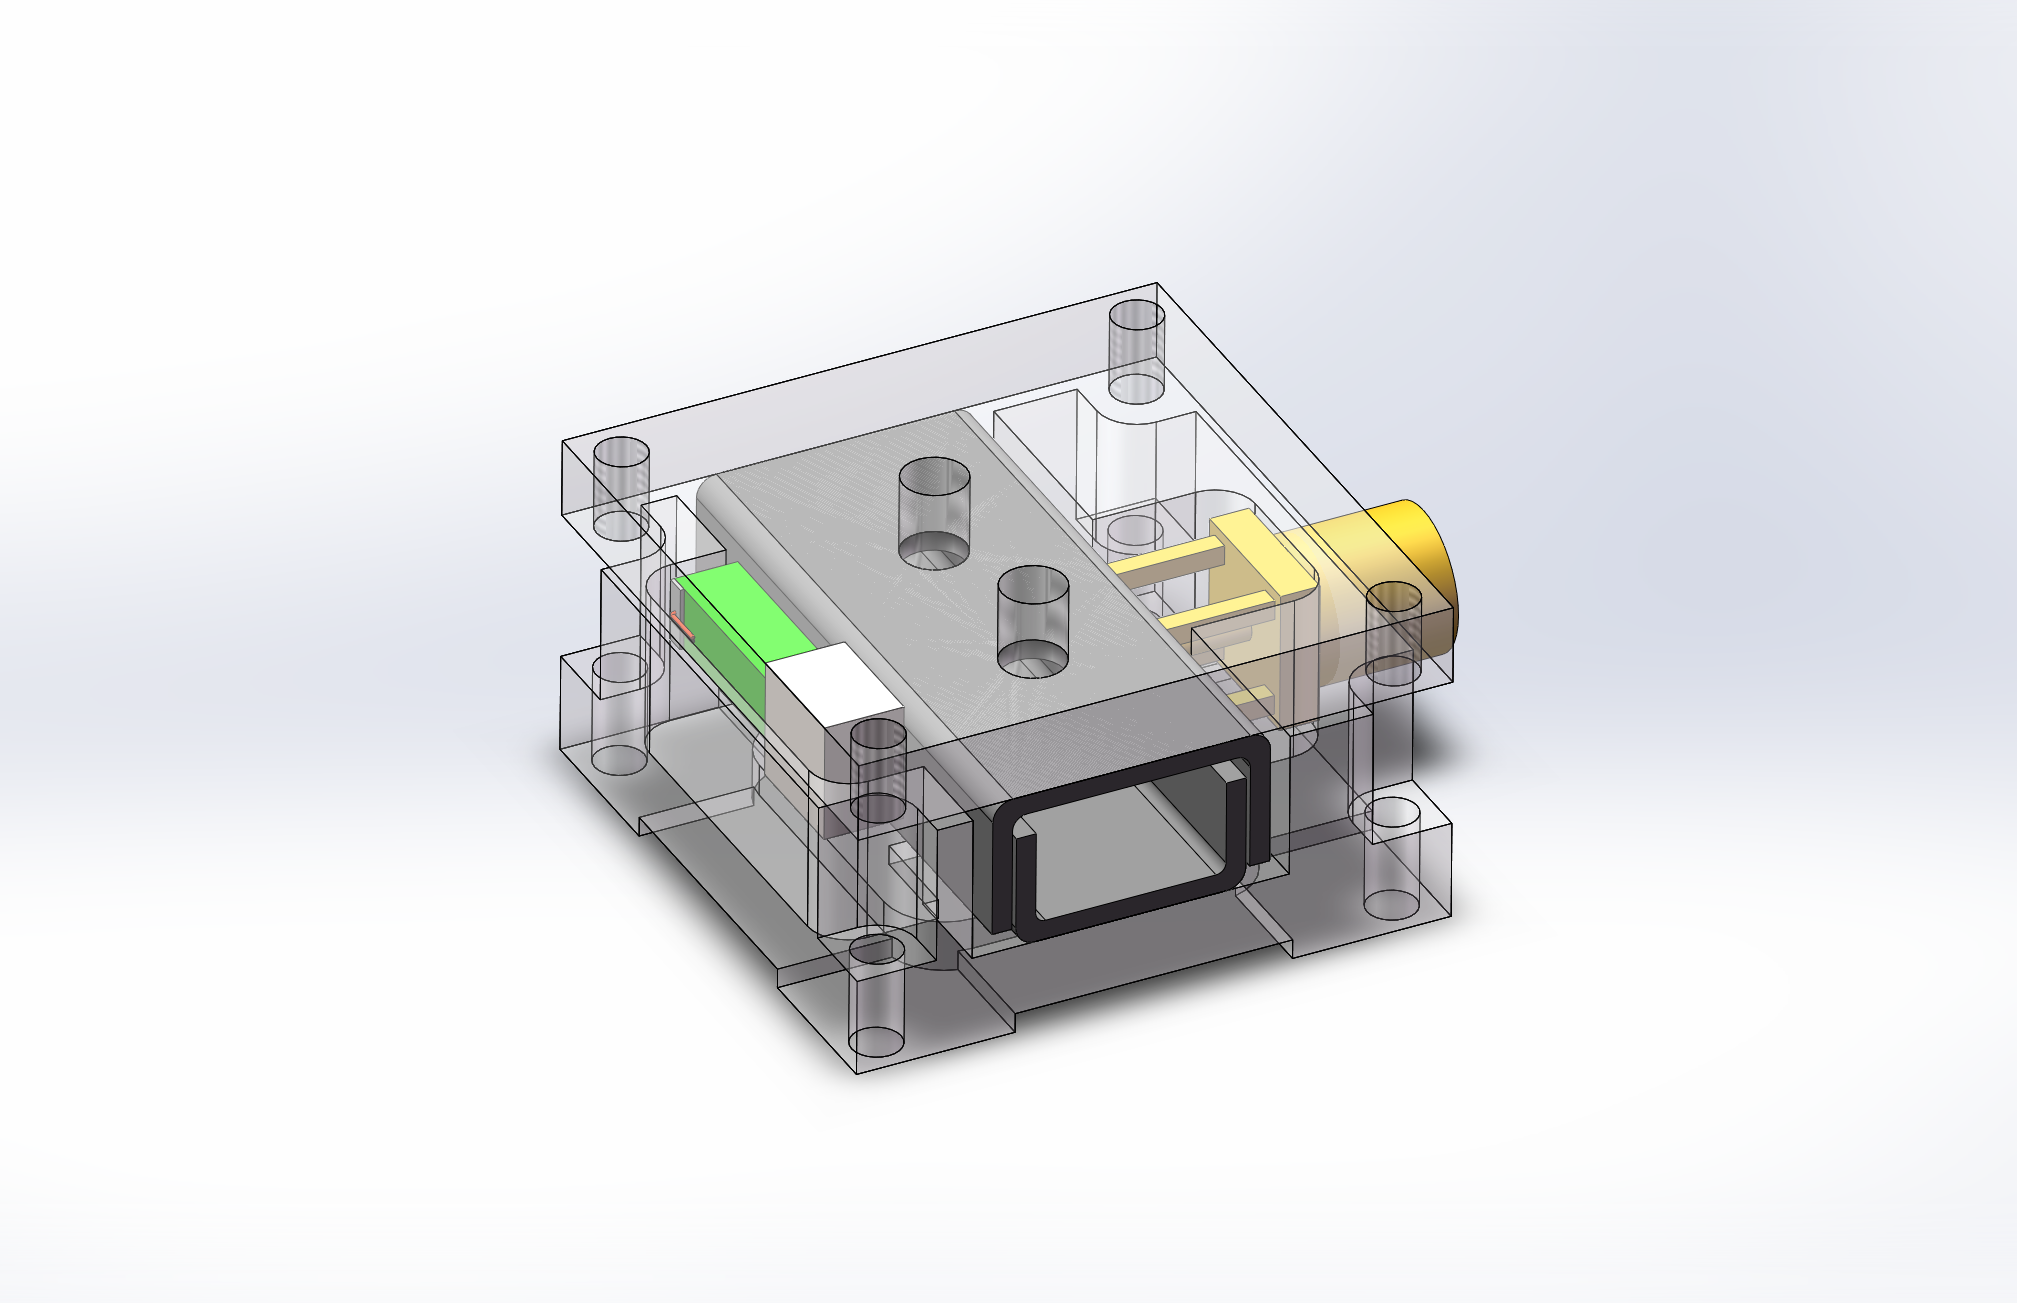
\includegraphics[width=\textwidth,clip,trim=50 30 30 30]{fig18.png}};
				\begin{scope}[x={(image.south east)},y={(image.north west)}]
					% 建立相对坐标系
					%							\draw[help lines,xstep=.1,ystep=.1] (0,0) grid (1,1);
					%							\foreach \x in {0,1,...,9} { \node [anchor=north] at (\x/10,0) {0.\x}; }
					%							\foreach \y in {0,1,...,9} { \node [anchor=east] at (0,\y/10) {0.\y}; }
					
					\draw [very thick,dotted](0.35,0.45)rectangle(0.41,0.51);
					\draw [ultra thick](0.35,0.45)--(0.2,0.29);
					\draw [very thick,dotted](0.3,0.54)rectangle(0.36,0.59);
					\draw [ultra thick](0.3,0.54)--(0.18,0.29);
					\node at(0.25,0.3)[below left]{粘合点};
					
					\draw [very thick,dotted](0.6,0.53)rectangle(0.68,0.62);
					\draw [ultra thick](0.68,0.58)--(0.75,0.62);
					\node at(0.73,0.62)[right]{粘合点};
					
					\draw [ultra thick,red](0.32,0.52)--(0.3,0.75);
					\node at(0.3,0.75)[above]{VCC};
					
					\draw [ultra thick,blue](0.32,0.52)--(0.2,0.5);
					\node at(0.2,0.5)[left]{GND};
					
					\draw [ultra thick,red](0.62,0.48)--(0.75,0.48);
					\node at(0.75,0.48)[right]{VCC};
					
					\draw [ultra thick,blue](0.56,0.58)--(0.68,0.75);
					\node at(0.68,0.75)[above]{GND};
					
					
				\end{scope}
				
			\end{tikzpicture}
			\caption{胶水粘合点与线路连接(水平)}
		\end{subfigure}
		\vskip 1em
		\begin{subfigure}{0.45\textwidth}
			\centering
			\begin{tikzpicture}
				\node[anchor=south west,inner sep=0] (image) at (0,0){
					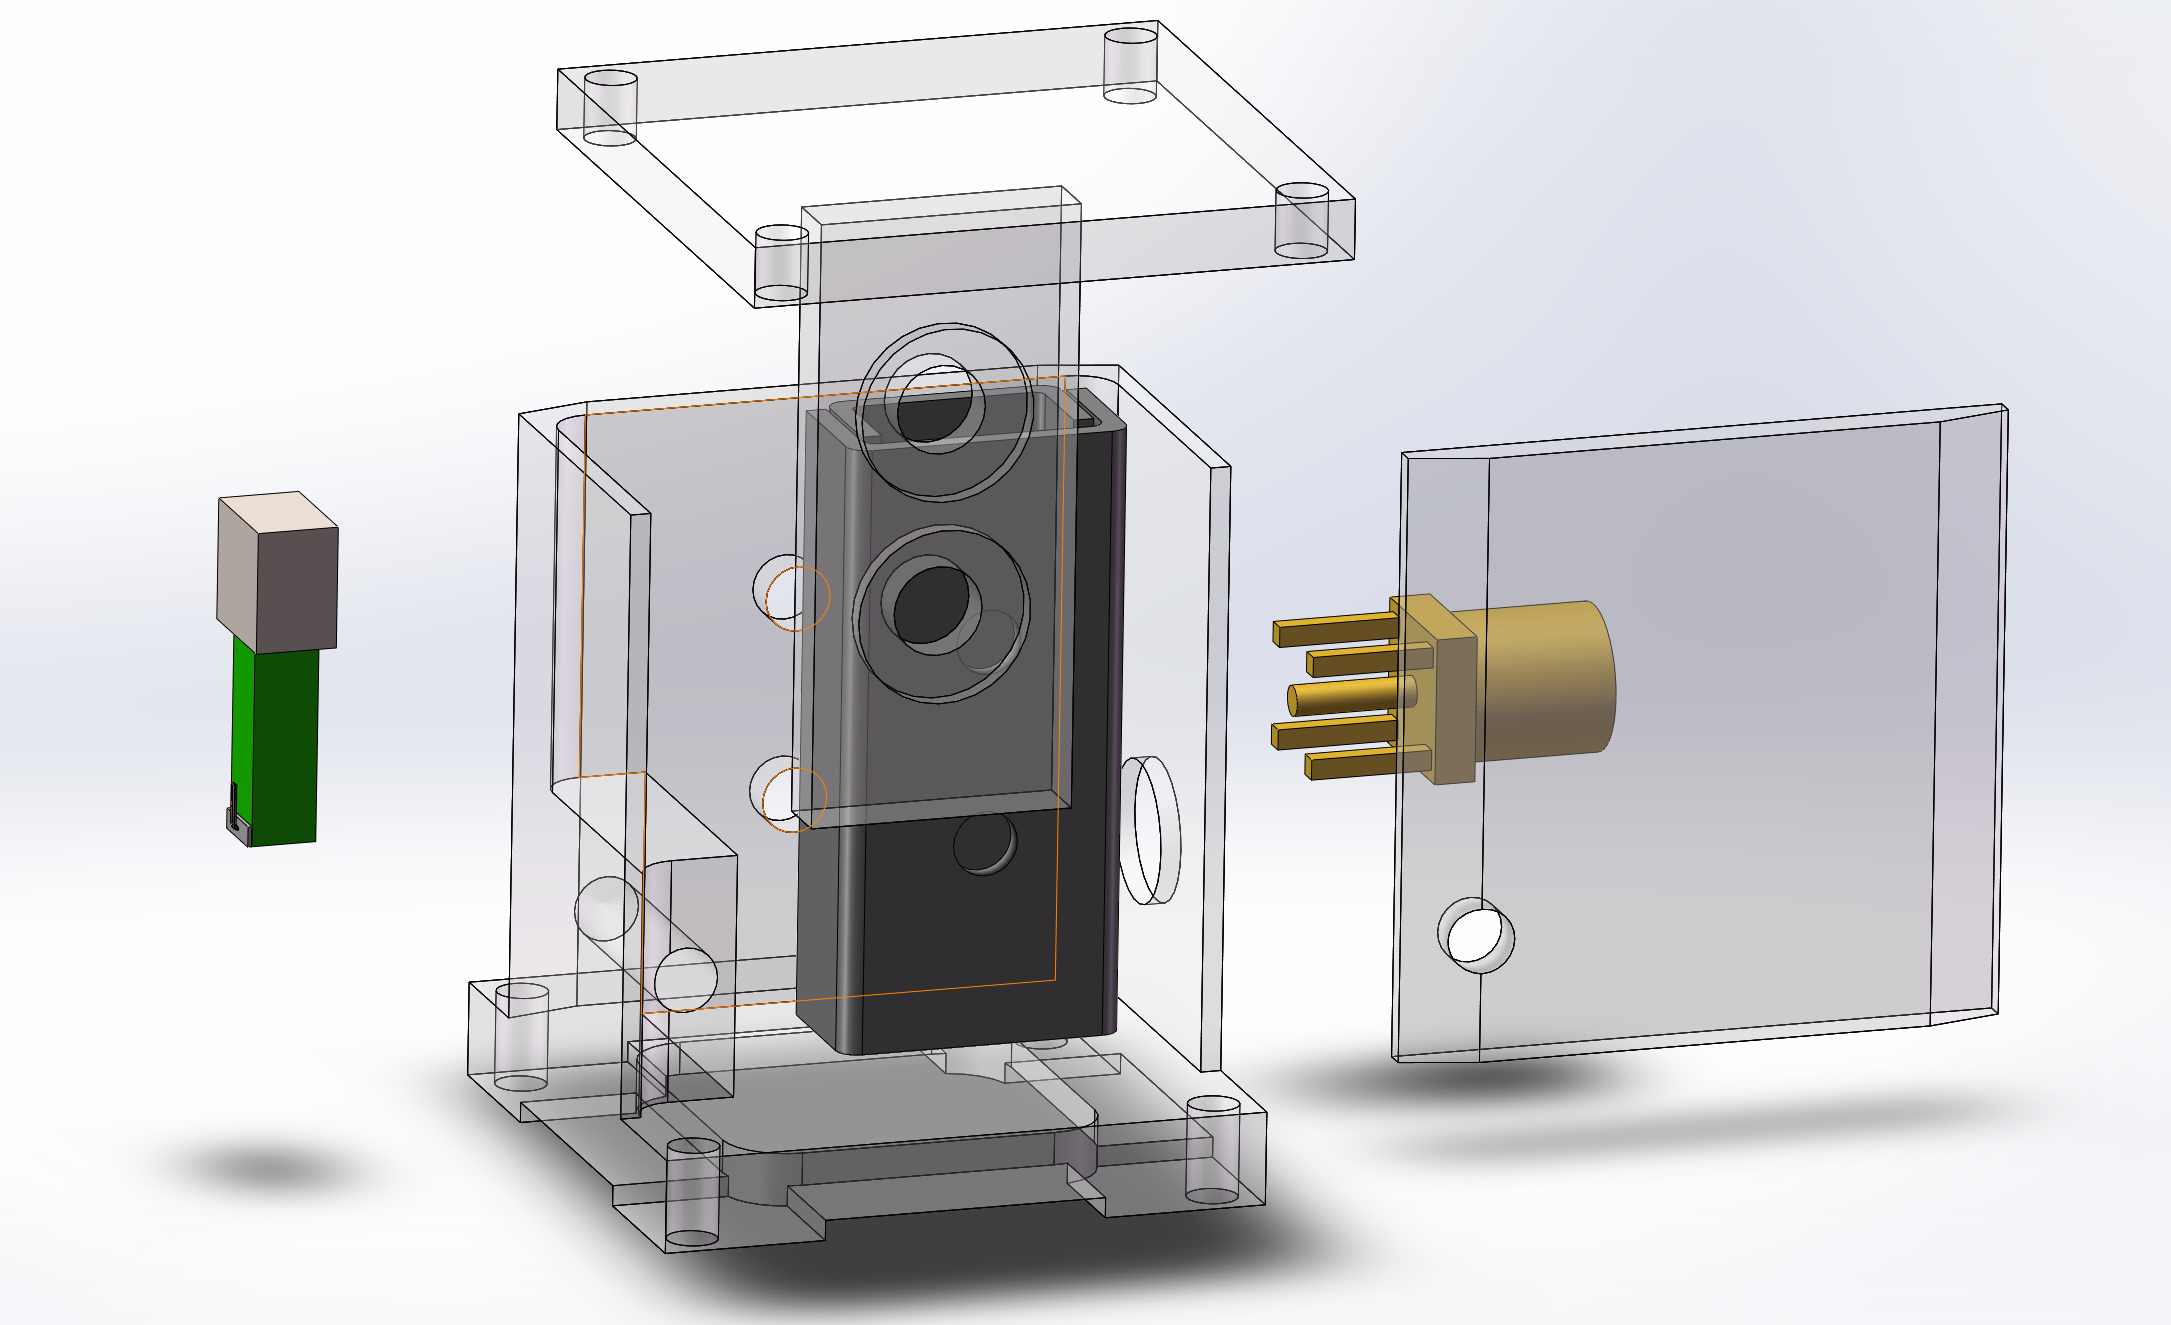
\includegraphics[width=\textwidth]{fig19.png}};
				\begin{scope}[x={(image.south east)},y={(image.north west)}]
					% 建立相对坐标系
					%							\draw[help lines,xstep=.1,ystep=.1] (0,0) grid (1,1);
					%							\foreach \x in {0,1,...,9} { \node [anchor=north] at (\x/10,0) {0.\x}; }
					%							\foreach \y in {0,1,...,9} { \node [anchor=east] at (0,\y/10) {0.\y}; }
					
					\draw [ultra thick](0.7,0.5)--(0.8,0.78);
					\node at(0.8,0.75)[above]{1:MMCX 座};
					
					\draw [ultra thick](0.13,0.4)--(0.13,0.3);
					\node at(0.13,0.3)[below]{2:压电晶体};
					\draw [ultra thick](0.13,0.6)--(0.13,0.7);
					\node at(0.13,0.7)[above]{2:磁铁};
					
					\draw [ultra thick](0.46,0.3)--(0.62,0.1);
					\node at(0.62,0.1)[right]{3:直线导轨};
					
					\draw [ultra thick](0.3,0.9)--(0.2,0.9);
					\node at(0.2,0.9)[left]{4:平台};
					
					\draw [ultra thick](0.3,0.1)--(0.2,0.1);
					\node at(0.2,0.1)[left]{底座};
					
					\draw [ultra thick](0.43,0.7)--(0.495,0.9);
					\draw [ultra thick](0.43,0.54)--(0.505,0.9);
					\node at(0.5,0.9)[above]{5:5$\times$M2};
					
					\node at(0.8,0.3){盖板};
					
				\end{scope}
			\end{tikzpicture}
			\caption{组装过程(垂直)}
		\end{subfigure}
		\hfill
		\begin{subfigure}{0.45\textwidth}
			\centering
			\begin{tikzpicture}[scale=0.75]
				\node[anchor=south west,inner sep=0] (image) at (0,0){
					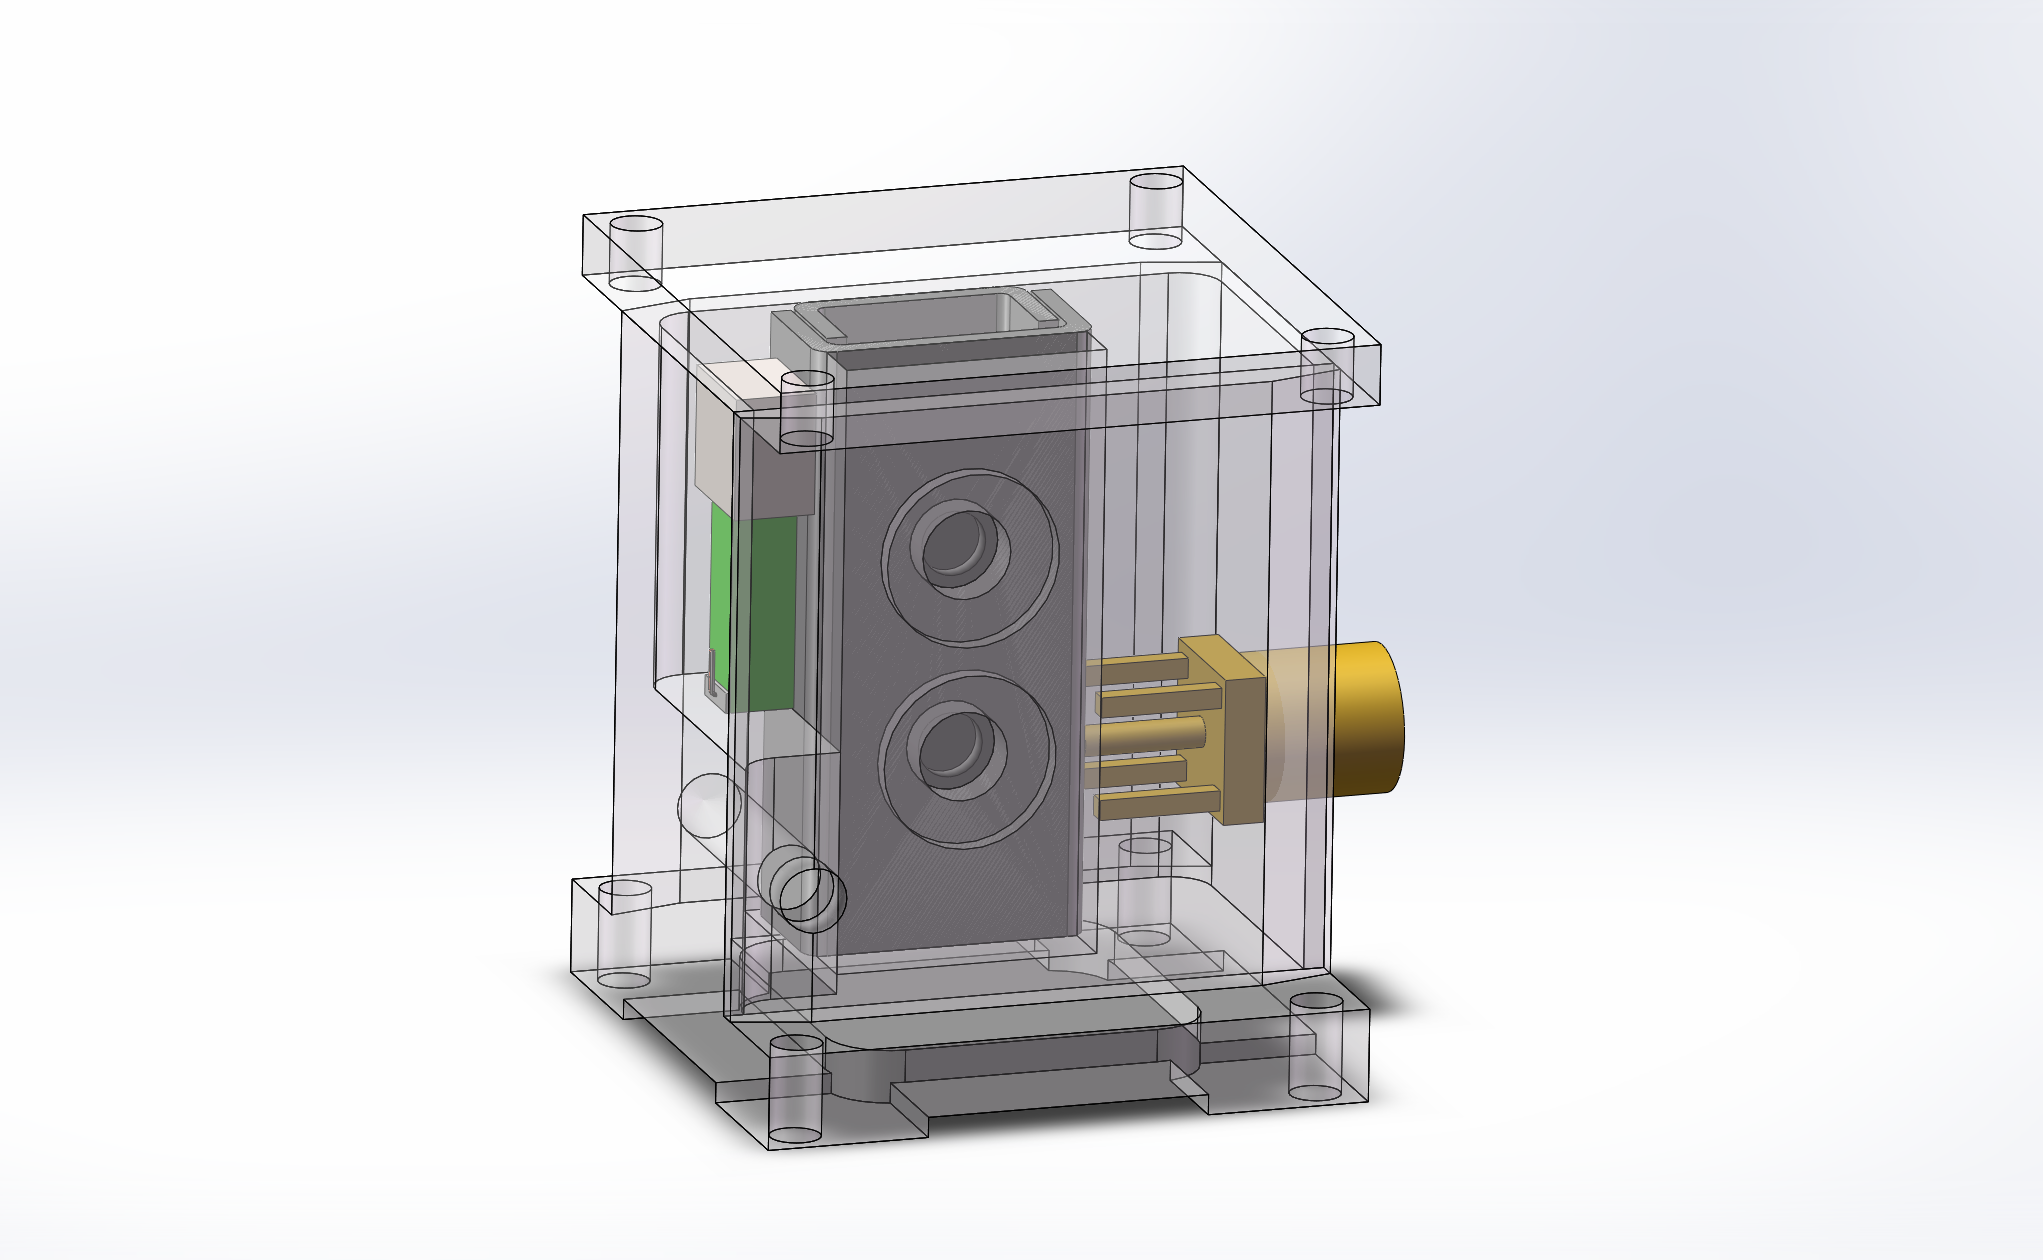
\includegraphics[width=\textwidth]{fig20.png}};
				\begin{scope}[x={(image.south east)},y={(image.north west)}]
					% 建立相对坐标系
					%							\draw[help lines,xstep=.1,ystep=.1] (0,0) grid (1,1);
					%							\foreach \x in {0,1,...,9} { \node [anchor=north] at (\x/10,0) {0.\x}; }
					%							\foreach \y in {0,1,...,9} { \node [anchor=east] at (0,\y/10) {0.\y}; }
					
					\draw [very thick,dotted](0.33,0.58)rectangle(0.4,0.61);
					\draw [ultra thick](0.33,0.58)--(0.18,0.29);
					\draw [very thick,dotted](0.33,0.42)rectangle(0.4,0.45);
					\draw [ultra thick](0.33,0.42)--(0.2,0.29);
					\node at(0.25,0.3)[below left]{粘合点};
					
					\draw [very thick,dotted](0.6,0.31)rectangle(0.66,0.51);
					\draw [ultra thick](0.66,0.51)--(0.75,0.62);
					\node at(0.73,0.62)[right]{粘合点};
					
					\draw [ultra thick,red](0.35,0.45)--(0.2,0.72);
					\node at(0.2,0.7)[above]{VCC};
					
					\draw [ultra thick,blue](0.35,0.45)--(0.2,0.5);
					\node at(0.2,0.5)[left]{GND};
					
					\draw [ultra thick,red](0.56,0.415)--(0.75,0.25);
					\node at(0.73,0.25)[right]{VCC};
					
					\draw [ultra thick,blue](0.56,0.47)--(0.56,0.8);
					\node at(0.56,0.78)[above]{GND};
					
				\end{scope}
				
			\end{tikzpicture}
			\caption{胶水粘合点与线路连接(垂直)}
			
		\end{subfigure}
		\caption{滑台组装示意图}
		\label{fig20}
	\end{figure}
	\vskip 1em
	
	
	
	\subsubsection{电子电路部分}
	按照电路设计文件印刷各个电路板并焊接元器件。其中 TIA 板、转接板需固定在 STM 主体上;样品平台板固定在压电滑台上;电源板、压电滑台驱动板、扫描头驱动板以及 ADC \& MCU 板则按照图 \ref{fig8} 所示使用 20 根六角铜柱层叠固定。各电路板接口之间使用 MMCX 同轴线与 IDC 排线连接,线型及连接方式见表 \ref{tab2}。
	
	\begin{figure}[htbp]
		\centering
		\begin{tikzpicture}
			begin{tikzpicture}
			\node[anchor=south west,inner sep=0] (image) at (0,0) {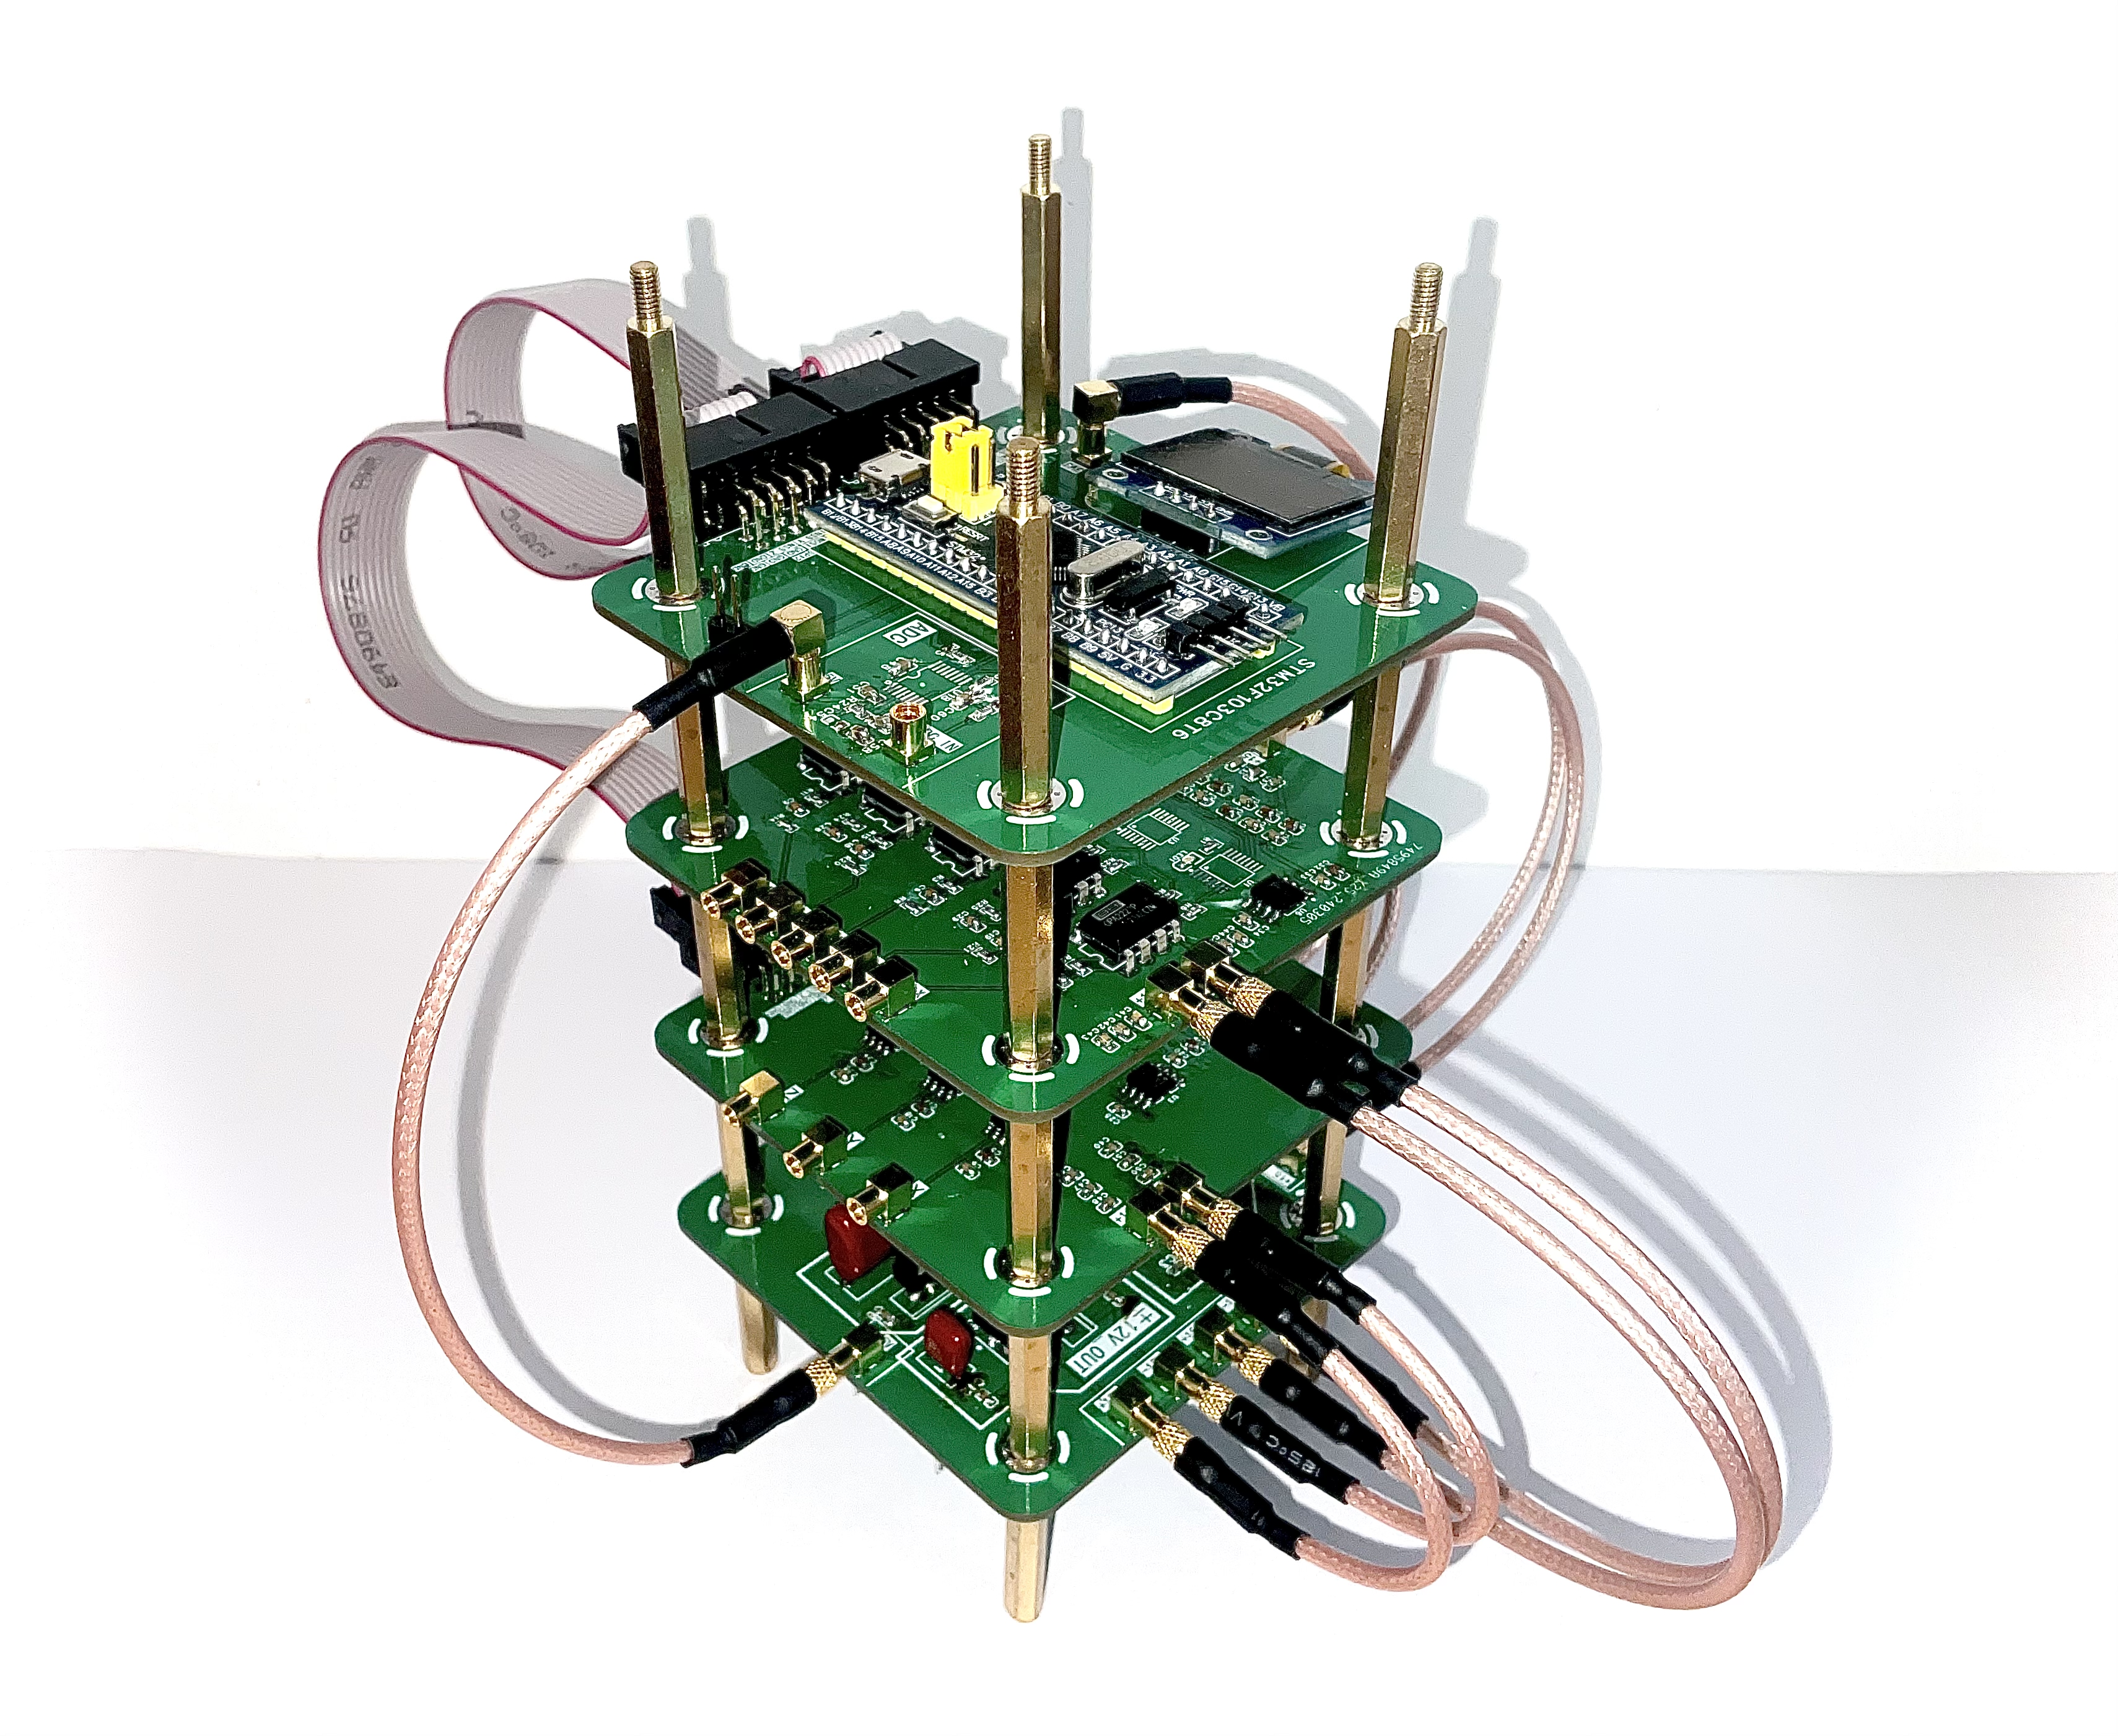
\includegraphics[width=0.8\textwidth]{fig13.jpg}};
			\begin{scope}[x={(image.south east)},y={(image.north west)}]
				%					 建立相对坐标系
				%					\draw[help lines,xstep=.1,ystep=.1] (0,0) grid (1,1);
				%					\foreach \x in {0,1,...,9} { \node [anchor=north] at (\x/10,0) {0.\x}; }
				%					\foreach \y in {0,1,...,9} { \node [anchor=east] at (0,\y/10) {0.\y}; }
				%					 作图命令
				\draw[black,ultra thick] (0.32,0.3)--(0.23,0.2)--(0.15,0.2);
				\node at(0.15,0.2)[left]{电源板};
				
				\draw[black,ultra thick,shift={(0,0.1)}] (0.32,0.3)--(0.23,0.2)--(0.15,0.2);
				\node at(0.15,0.22)[left,shift={(0,0.1)}]{压电滑台};
				\node at(0.15,0.18)[left,shift={(0,0.1)}]{驱动板};
				
				\draw[black,ultra thick,shift={(0,0.21)}] (0.32,0.3)--(0.23,0.2)--(0.15,0.2);
				\node at(0.15,0.22)[left,shift={(0,0.21)}]{扫描头};
				\node at(0.15,0.18)[left,shift={(0,0.21)}]{驱动板};
				
				\draw[black,ultra thick,shift={(0,0.36)}] (0.32,0.3)--(0.23,0.2)--(0.15,0.2);
				\node at(0.15,0.22)[left,shift={(0,0.36)}]{ADC \&};
				\node at(0.15,0.18)[left,shift={(0,0.36)}]{MCU 板};
				
				\draw [red,rounded corners,ultra thick](0.33,0.25)rectangle(0.44,0.63);
				\draw[red,ultra thick] (0.36,0.63)--(0.32,0.75)--(0.15,0.75);
				\node at(0.15,0.77)[left]{MMCX};
				\node at(0.15,0.73)[left]{输入输出};
				
				\draw[black,ultra thick] (0.72,0.32)--(0.8,0.4)--(0.85,0.4);
				\node at(0.85,0.42)[right]{MMCX};
				\node at(0.85,0.38)[right]{同轴线};
				
				\draw[black,ultra thick] (0.55,0.65)--(0.75,0.75)--(0.85,0.75);
				\node at(0.85,0.75)[right]{MCU};
				
			\end{scope}
		\end{tikzpicture}
		\caption{电路板实物图}
		\label{fig8}
	\end{figure}
	
	\begin{table}[htbp]
		\small
		\caption{DIY-STM 接线表}
		\centering
		\begin{tabular}{ccccc}
			\toprule[1.5pt]
			\textbf{\quad 源 PCB\quad} & \textbf{\quad 目标 PCB\quad} & \textbf{\quad 源接口\quad} & \textbf{\; 目标接口\;} & \textbf{\quad 类型\quad}  \\ 
			\midrule[0.8pt]
			Power\_Board & Motor\_Board & 3V3\_1 & 3V3 & MMCX-MMCX \\
			Power\_Board & Motor\_Board & +12 / -12V & +12V / 12V & MMCX-MMCX \\
			Power\_Board & Motor\_Board & +15\_1 / -15\_1 & +15V / -15V & MMCX-MMCX \\
			\midrule[0.1pt]
			Power\_Board & Controller\_Board & 3V3\_2 & 3V3 & MMCX-MMCX \\
			Power\_Board & Controller\_Board & +15\_2 / -15V\_2 & +15V / -15V & MMCX-MMCX \\
			Power\_Board & Controller\_Board & +15\_3 / -15V\_3 & +15V / -15V & MMCX-MMCX \\
			\midrule[0.1pt]
			Power\_Board & ADC\_And\_MCU\_Board & 3V3\_3 & 3V3 & MMCX-MMCX \\
			Power\_Board & ADC\_And\_MCU\_Board & 5V & 5V & MMCX-MMCX \\
			\midrule[0.1pt]
			Motor\_Board & ADC\_And\_MCU\_Board & SPI2 & SPI2 & IDC-IDC$^\text{1}$ \\
			Controller\_Board & ADC\_And\_MCU\_Board & SPI1 & SPI1 & IDC-IDC \\
			\midrule[0.1pt]
			Power\_Board & Connector\_Board & +15\_4 / -15V\_4 & +15V / -15V & MMCX-MMCX \\
			Power\_Board & Connector\_Board & GND & GND & MMCX-MMCX \\
			\midrule[0.1pt]
			Motor\_Board & PZT\_Slide\_Table & X / Y / Z & X / Y / Z & MMCX-MMCX \\
			\multirow{2}*{Controller\_Board} & \multirow{2}*{Connector\_Board} & Z+X / Z-X & Z+X / Z-X & \multirow{2}*{MMCX-MMCX} \\
			~ & & Z+Y / Z-Y & Z+Y / Z-Y & \\
			\midrule[0.1pt]
			Connector\_Board & ADC\_And\_MCU\_Board & ADC & ADC\_IN & MMCX-MMCX \\
			\bottomrule[1.5pt]
		\end{tabular}
		\\\vskip 1mm
		\begin{minipage}{0.95\linewidth}
			附注 1:IDC 插头型号为:2.54-2$\times$5P。
		\end{minipage}
		\label{tab2}
	\end{table}
	\vskip 1em
	
	
	
	
	
	\subsubsection{组装显微镜主体}
	显微镜主体组装共分为五个步骤:
	\begin{enumerate}
		\item 将组装好的扫描头放入基座圆形凹槽中(X 轴处于水平状态),接着将扫描头固定件压入凹槽内,使用两颗 M2 螺丝固定。
		\item 把 TIA 板放入扫描头正下方凹槽内,盖上盖板并用两颗 M2 螺丝固定。
		\item 将磁铁\footnote{磁铁型号为:ACTD-B2-W10-H5-T2。}按标识固定在样品平台板上,保证两者之间的电气连接。
		\item 使用四颗 M1.6 螺丝将样品平台板固定在压电滑台上,再用四颗 M1.6 螺丝将压电滑台固定在基座上,使磁铁靠近扫描头一侧。
		\item 利用四颗 M2 螺丝将转接板固定在基座外侧。
	\end{enumerate}
	组装完成后的显微镜主体如图 \ref{fig9} 所示。各部分连接应确保稳固可靠,并检查所有连接是否正确无误。
	\begin{figure}[htbp]
		\centering
		\hfill
		\begin{subfigure}{0.4\textwidth}
			\centering
			\begin{tikzpicture}
				\node[anchor=south west,inner sep=0] (image) at (0,0) {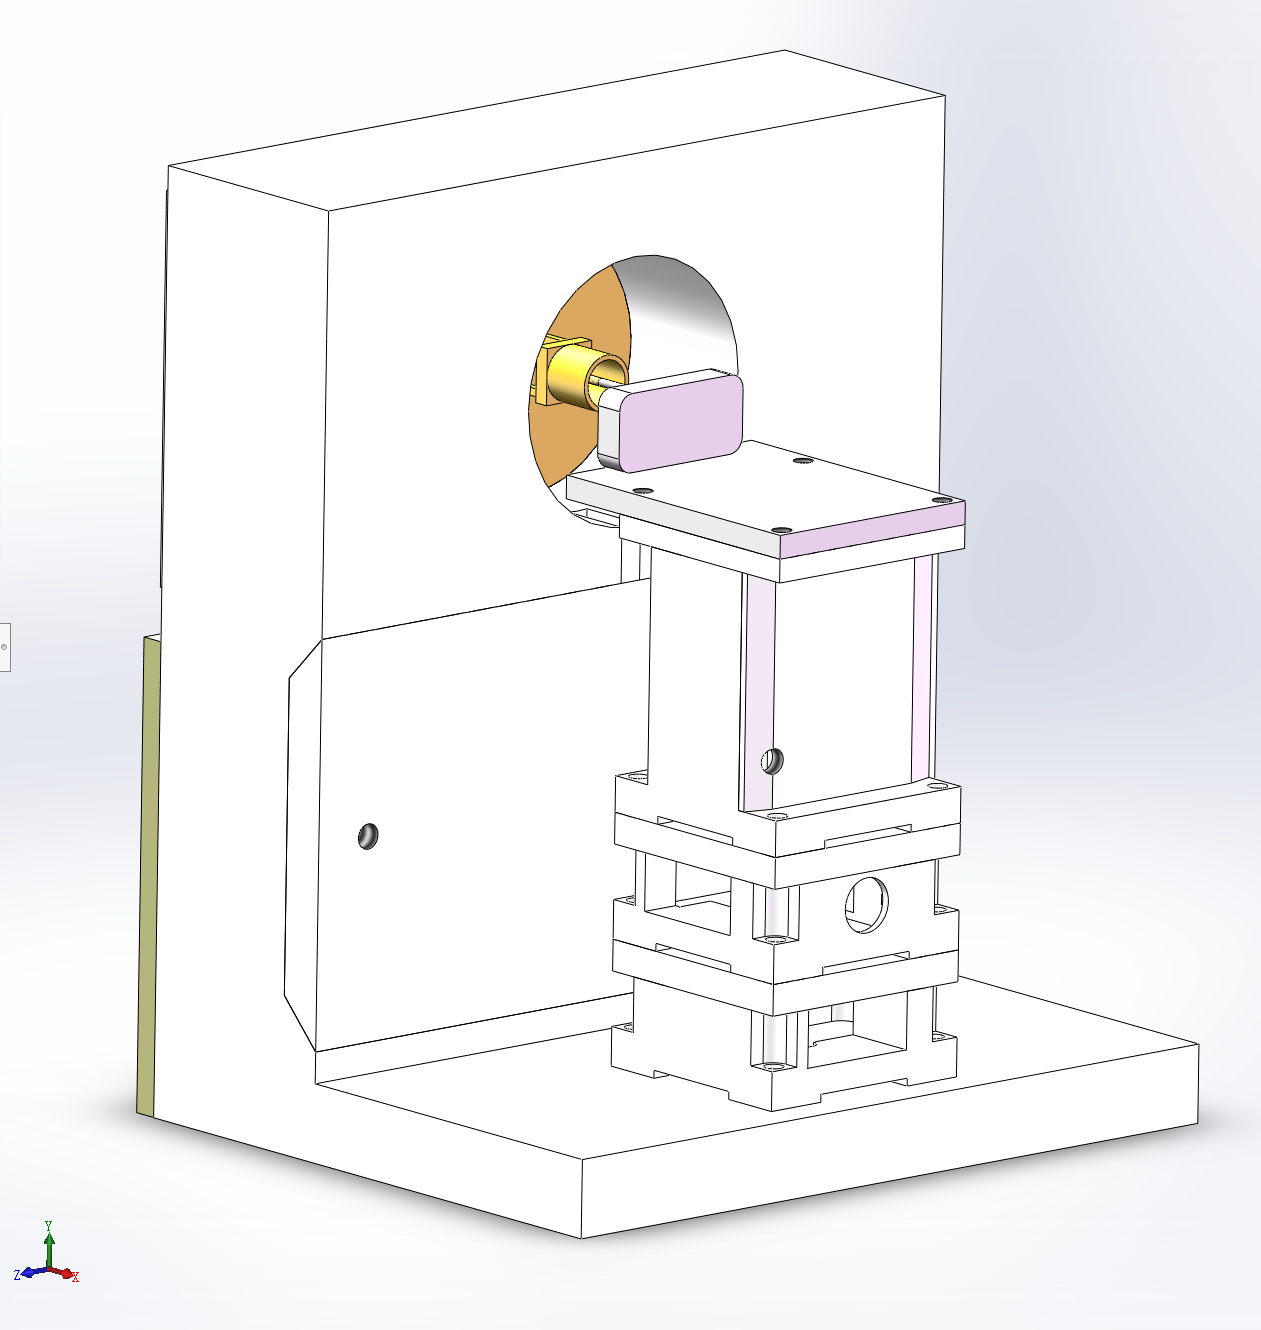
\includegraphics[width=\textwidth]{fig11.png}};
				\begin{scope}[x={(image.south east)},y={(image.north west)}]
					%%					 建立相对坐标系
					%						\draw[help lines,xstep=.1,ystep=.1] (0,0) grid (1,1);
					%						\foreach \x in {0,1,...,9} { \node [anchor=north] at (\x/10,0) {0.\x}; }
					%						\foreach \y in {0,1,...,9} { \node [anchor=east] at (0,\y/10) {0.\y}; }
					%%					 作图命令
					\draw [|<->|,ultra thick,black](0.08,0.157)--(0.08,0.877);
					\node at(0.05,0.5)[rotate=90]{60mm};
					
					\draw [|<->|,ultra thick,black](0.11,0.128)--(0.45,0.032);
					\node at(0.25,0.05)[rotate=-15]{40mm};
					
					\draw [|<->|,ultra thick,black](0.468,0.03)--(0.955,0.124);
					\node at(0.75,0.05)[rotate=11]{50mm};
					
				\end{scope}
			\end{tikzpicture}
			\caption{3D 渲染模型(正)}
		\end{subfigure}\hfill
		\begin{subfigure}{0.37\textwidth}
			\centering
			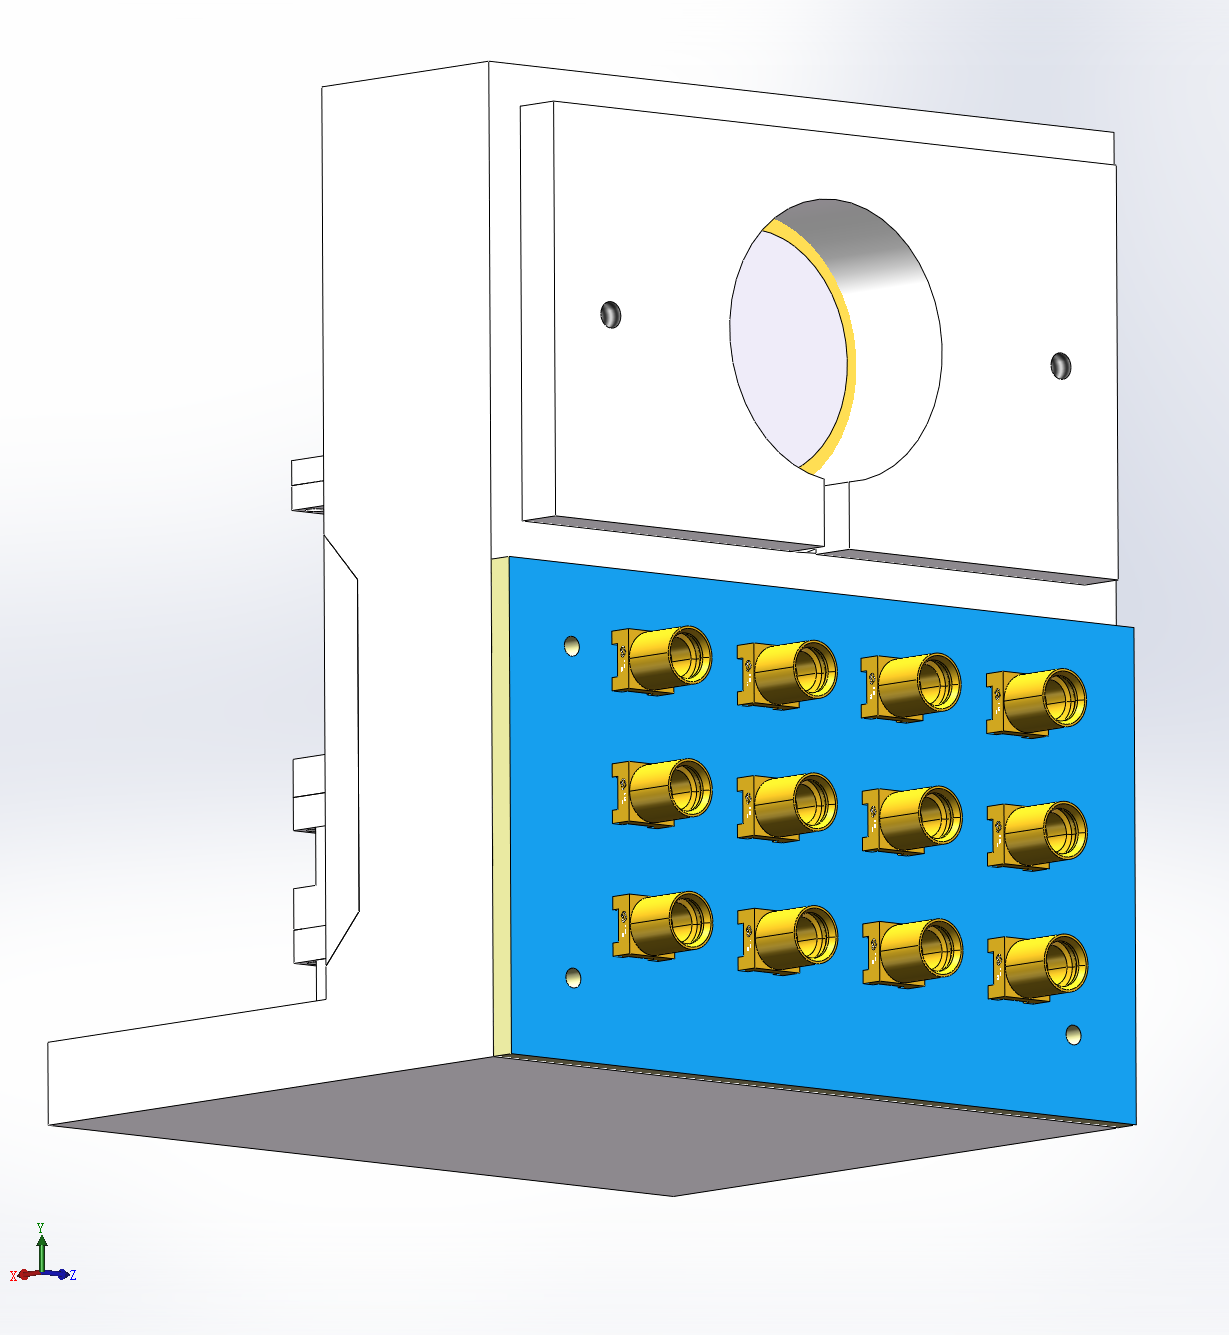
\includegraphics[width=\linewidth]{fig12.png}
			\caption{3D 渲染模型(反)}
		\end{subfigure}
		\hfill
		%				\vskip 1em
		%				\hfill
		%				\begin{subfigure}{0.4\textwidth}
			%					\centering
			%					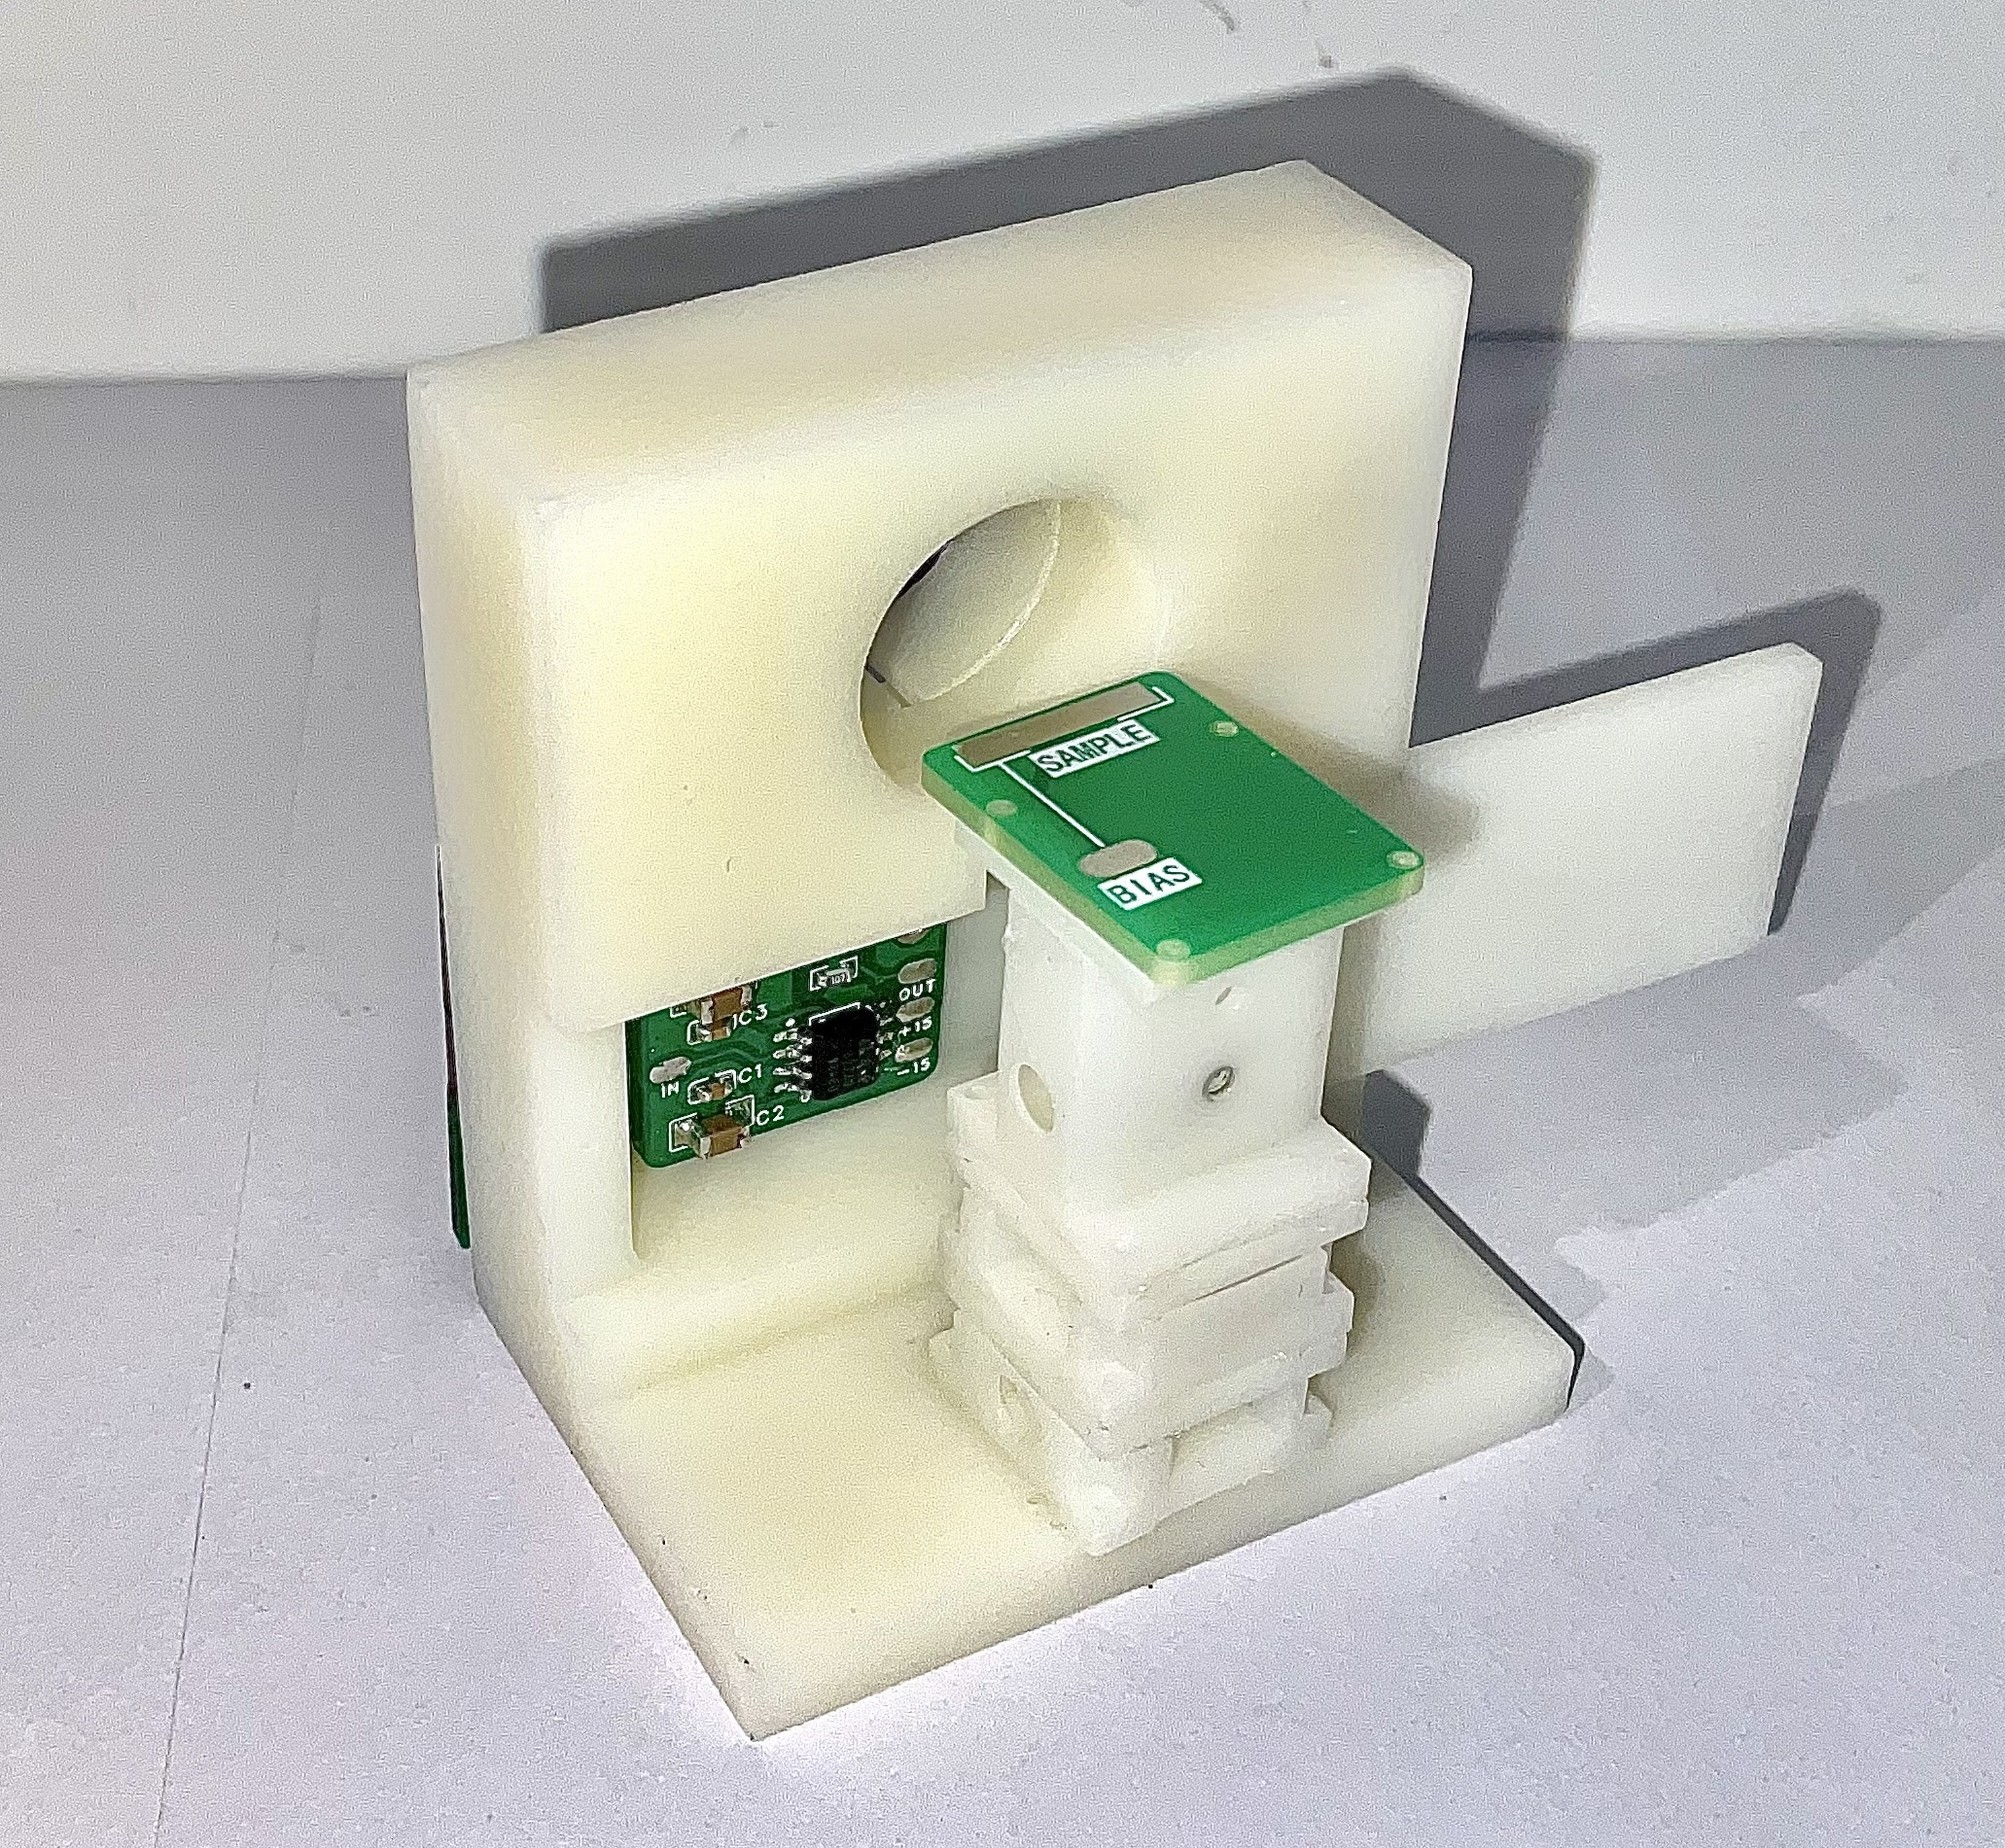
\includegraphics[width=\linewidth]{fig15.jpg}
			%					\caption{实物模型(正)}
			%				\end{subfigure}\hfill
		%				\begin{subfigure}{0.4\textwidth}
			%					\centering
			%					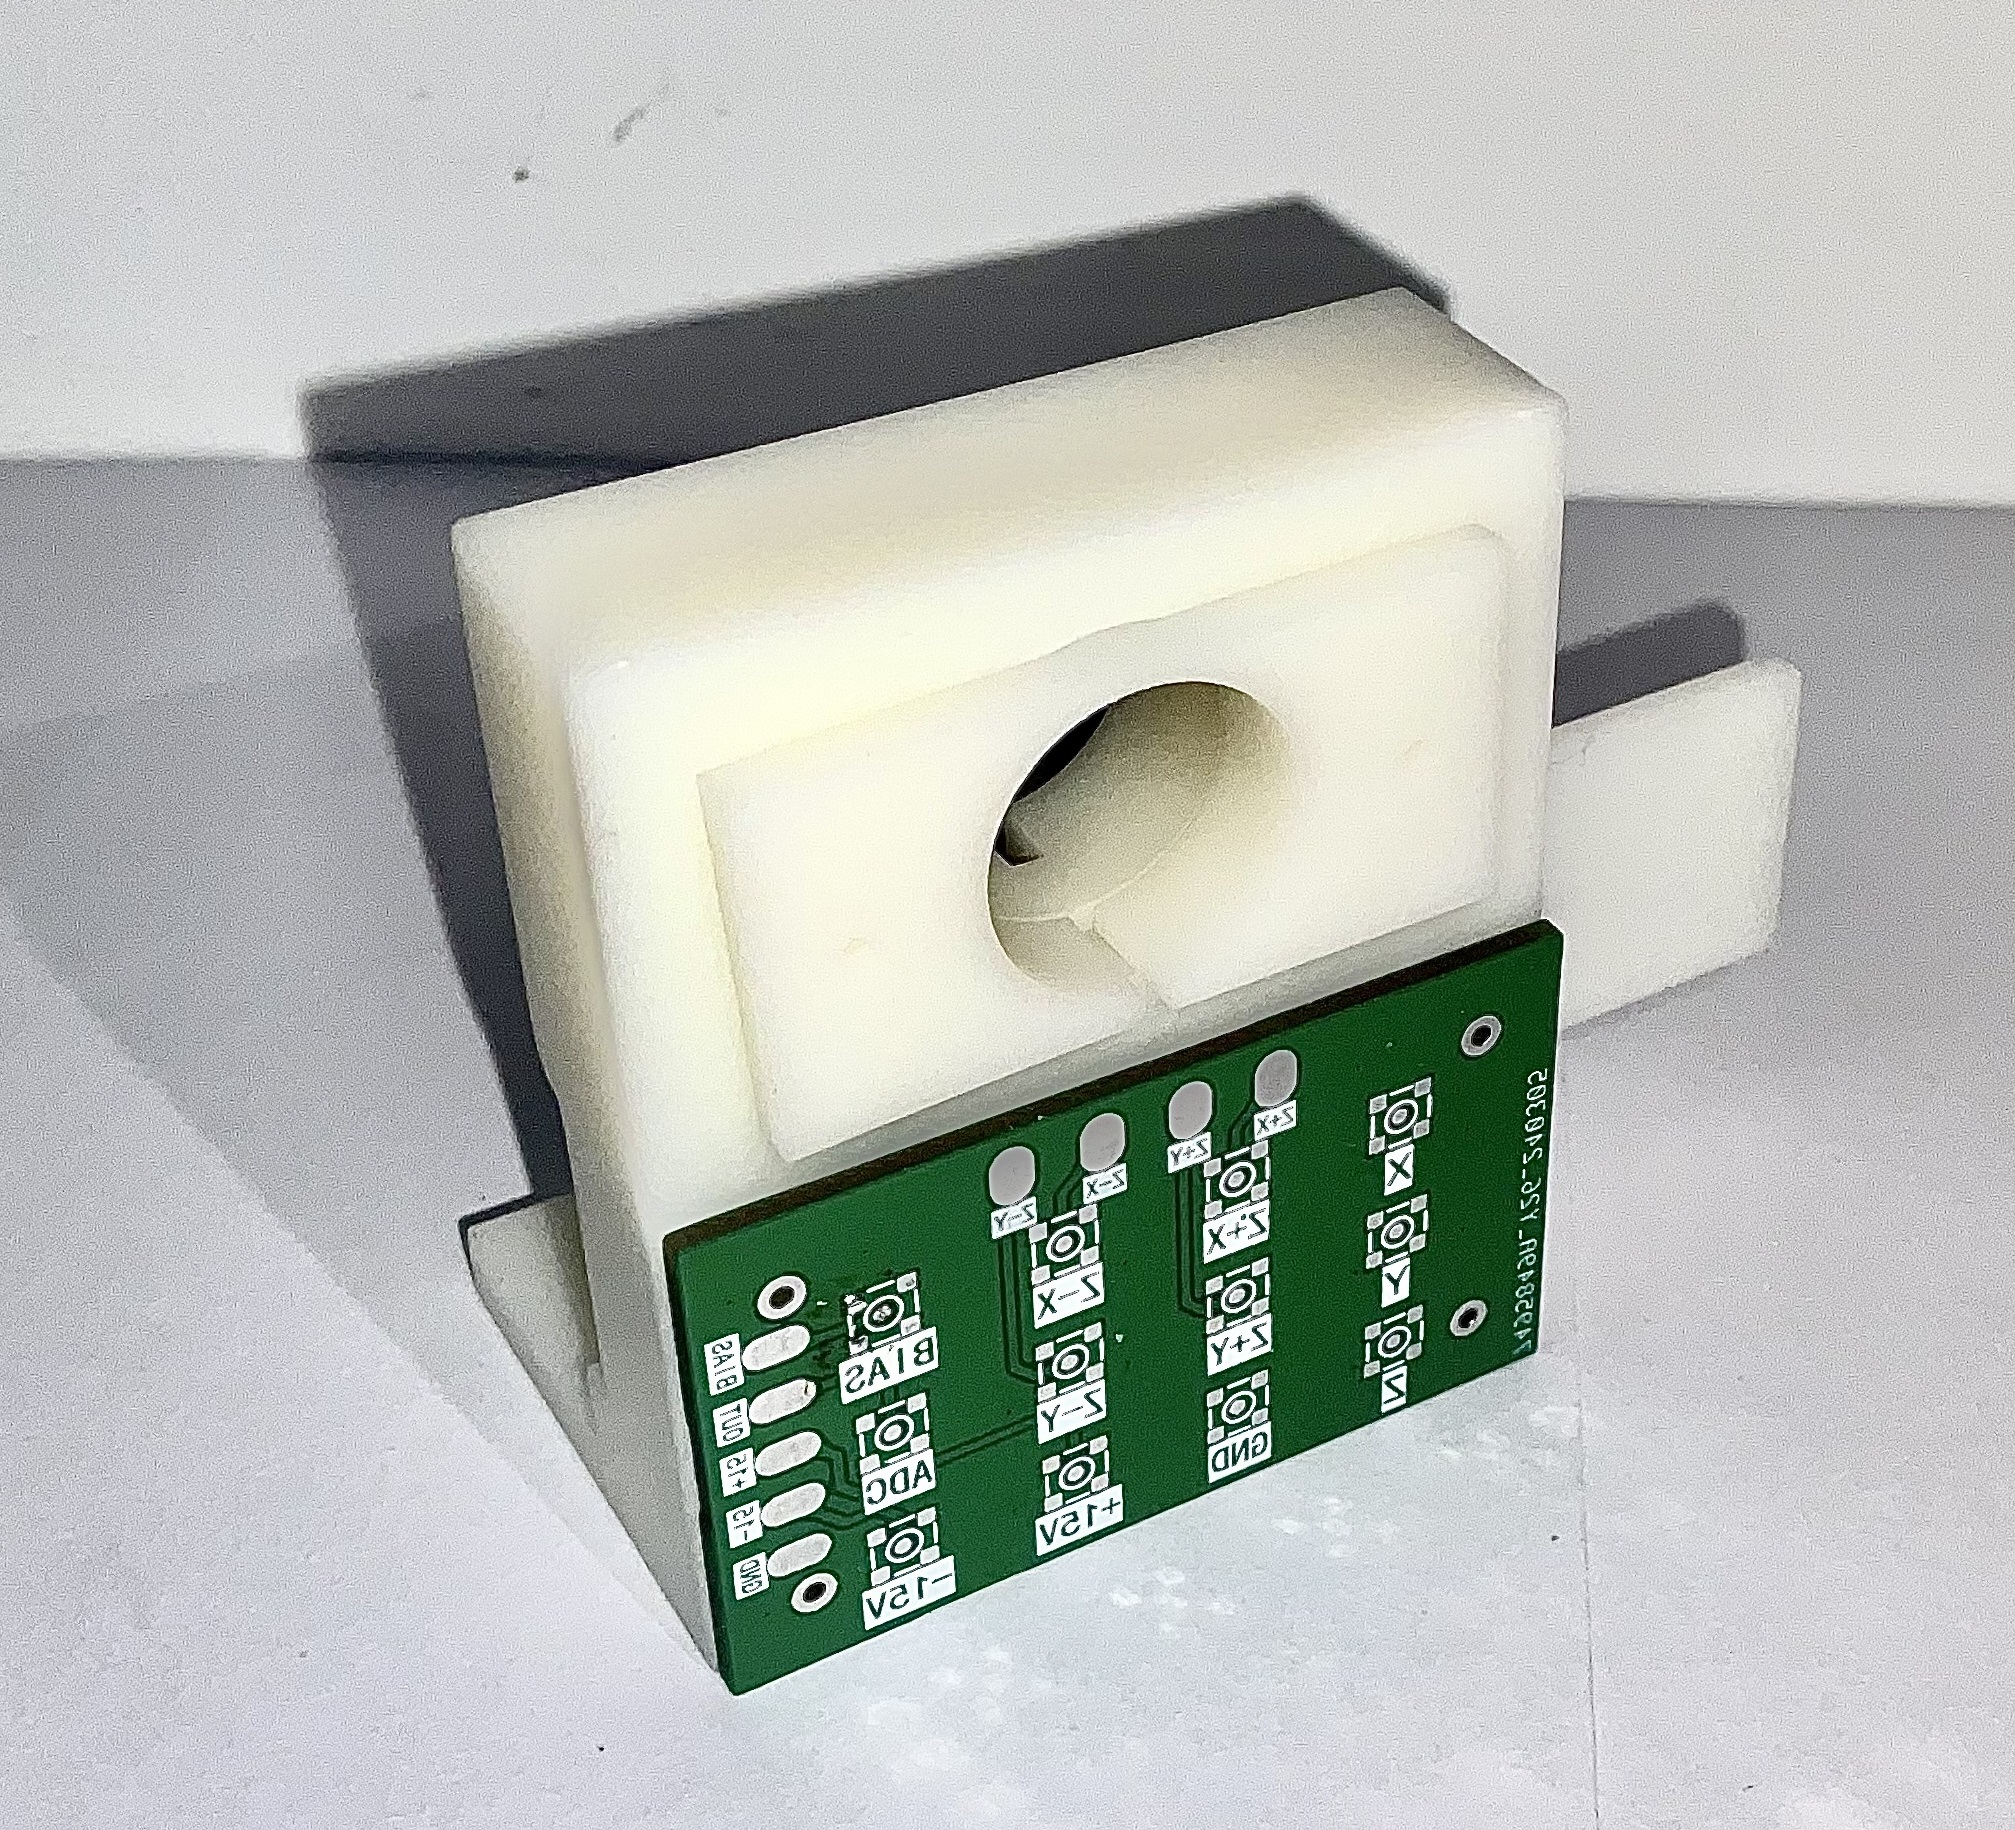
\includegraphics[width=\linewidth]{fig14.jpg}
			%					\caption{实物模型(反)}
			%				\end{subfigure}
		%				\hfill
		\caption{DIY-STM 主体示意图}
		\label{fig9}
	\end{figure}
	\vskip 1em
	
	
	
	
	\subsubsection{构建完整 STM 系统}
	为了构建一个完整的 STM 系统,我们需要将各个部分组合起来。首先选择一个无风、温度相对恒定的房间,安装减震系统。使用合适长度的 MMXC 同轴线将电路板的输出接口与 STM 主体相连,然后将 STM 主体放入一个合适的密封亚克力盒中并置于减震平台上。使用 CH340 与杜邦线连接电脑与 ADC \& MCU 板上的 USART 接口,最后使用 USB-A 为电路板提供 5V 供电。至此我们完成了 STM 系统的完整构建。
	
	
	
	\subsubsection{系统调试与运行}
	为了保证 STM 的正常运行,需要先对系统进行调试。安置样品并在电脑启动控制软件,在软件中选择串口并连接。接着设置合适的电压范围与步长测试压电滑台能否正常运行,如果可以正常运行,则执行 Approach 命令开始进近。进近过程中需观察 Current(隧穿电流)的状态以保证不会撞针。然后控制改变扫描头 Z 通道电压,若隧穿电流发生相应变化,则说明进近完成,可以开始曲线测试与图像扫描。此外,还应检查扫描结果以评估显微镜运行状态。
	
	
	
	
	
	
	
	
	
	
	
	\clearpage
	\setcounter{section}{5}	 	%这里根据结论是第几章来设置
	\setcounter{subsection}{0}	%重新计数子章节
	
	
	\section*{结论}
	\phantomsection
	\addcontentsline{toc}{section}{结论} % 将无标号章节添加至目录
	\setParDis %设置段间距为 0
	\subsection{应用前景}
	自制 STM 项目不仅可以在技术上验证低成本实现原子级分辨率成像的可行性,也能为纳米科学领域的研究和教育提供新的工具。通过自制 STM,研究人员能够更加方便地在实验室中探索物质表面的微观结构,这对于新材料的开发、表面科学的研究以及纳米技术的应用都具有重要意义。在教育领域,自制 STM 可以作为辅助教学工具,帮助学生直观理解量子力学和纳米技术的概念,激发他们对科学研究的兴趣。此外,借助自制 STM 的开放性,其为全球科学社区提供了一个共享知识和资源的途径,有助于推动全球范围内相关科学的合作与创新。
	
	
	\subsection{市场需求与商业化}
	随着纳米技术的快速发展,对于能够提供高分辨率表面分析的仪器需求日益增长。自制 STM 因其低成本、容易操作的特点,具有很强的的市场竞争潜力,尤其是在教育和小型研究机构中。自制 STM 可以作为一种经济实惠的科研工具,满足基础研究和教学的需求。此外,随着自制 STM 技术的优化与成熟,其商业化前景也将逐渐明朗。通过与工业界合作,可以将自制 STM 技术转化为商业产品,为更广泛的学科提供服务,如实验教育、材料科学、生物医学和半导体工业等诸多领域。
	
	
	\subsection{优劣分析与未来优化}
	自制 STM 项目虽然在成本和操作性方面具有明显优势,但也存在一些局限性。例如,与商业级 STM 系统相比,自制 STM 可能在成像精度、长期可靠性方面存在不足。此外,自制 STM 的维护和升级可能需要用户具备一定的技术背景,这可能限制了其在非专业用户中的普及。
	
	鉴于此,未来的工作可以集中在改进自制 STM 的设计、提高其性能和用户体验上。例如,通过采用更先进的材料和制造技术,可以提高 STM 的结构稳定性和测量精度。同时,开发更加直观易用的用户界面和软件工具,可以降低操作难度,使 STM 更加适合非专业用户使用。另外通过社区合作和开源共享,可以集合更多人的智慧,共同推动自制 STM 技术的发展和完善。
	
	
%====================正文====================
	
	
%====================参考文献====================
\newpage
\phantomsection
\section*{参考文献} % section*生成无标号章节题目
\setParDis %设置段间距为 0
\addcontentsline{toc}{section}{参考文献} % 将无标号章节添加至目录
\begingroup  % 去掉thebibliography环境自带的“参考文献”标题
\renewcommand{\section}[2]{} 
\begin
\begin{thebibliography}{25}
	\bibitem{ref1} 庞宗强.组合扫描探针显微镜系统研制[D].合肥:中国科学技术大学,2010.
	
	\bibitem{ref2} 陆轻铀.新型强力压电马达及其在恶劣条件下原子成像中的应用[J].物理, 2017,3:168-177.
	
	\bibitem{ref3} 夏志刚.高稳定与高重复电化学扫描隧道显微镜研制[D].合肥:中国科学技术大学, 2014.
	
	\bibitem{ref4} Pan S H, Hudson E W, Davis J C. $^\text{3}$He refrigerator based very low temperature scanning tunnelingmicroscope[J]. Review of Science Instruments, 1999, 70(2):1459-1463.
	
	\bibitem{ref5} Meckler S, Gyamfi M, Pietzsch O, et al. A low-temperature spin-polarized scanning tunneling microscope operating in a fully rotatable magnetic field[J]. Review of Science Instruments, 2009, 80: 023708.
	
	\bibitem{ref6} Pietzsch O, Kubetzka A, Haude D, et al. A low-temperature ultrahigh vacuumscanning tunneling microscope with a split-coil magnet and a rotary motionstepper motor for high spatialresolution studies of surface magnetism[J]. Review of Science Instruments, 2000, 71(2):424-430.
	
	\bibitem{ref7}Hug H J, Stiefel B, Schendel P J A, et al. A low temperature ultrahighvaccum scanning force microscope[J]. Review of Science Instruments, 1999, 70(9):3625-3640.
	
	\bibitem{ref8} 周泽清. 扫描隧道显微镜的研制及其应用研究[D]. 南京邮电大学, 2020.
	
	\bibitem{ref9} 江澄. 我国太赫兹扫描隧道显微镜系统研制实现突破[EB/OL]. (2022-02-25)[2024-04-06]. \href{https://www.cas.cn/syky/202202/t20220225\_4826270.shtml}{https://www.cas.cn/syky/202202/t20220225\_4826270.shtml}.
	
	\bibitem{ref10} Yan J H, Ma J J, Wang A W, et al. A time-shared switching scheme designed for multi-probe scanning tunneling microscope[J]. Review of Scientific Instruments, 2021, 92(10): 103702.
	
	\bibitem{ref11} D Berard. Home-Built STM[EB/OL]. 2014[2024-04-06]. \href{https://dberard.com/home-built-stm/}{https://dberard.com/home-built-stm/}.
	
	\bibitem{ref12} Alexander J D. Simple STM Project[EB/OL]. (2003-12)[2024-04-06]. \href{https://john-alexander42.github.io/simple-stm-web-page/}{https://john-alexander42.github.io/simple-stm-web-page/}.
	
	\bibitem{ref13} Alexander J D, Tortonese M, Nguyen T. Atomic force microscope with integrated optics for attachment to optical microscope: US005952657A[P]. 1999-09-14.
	
	\bibitem{ref14} Wallash A, Levit L B. Electrical breakdown and ESD phenomena for devices with nanometer-to-micron gaps[C]. SPIE MOEMS-MEMS. 2003. 
	
	\bibitem{ref15} Tirumala R, Go D B. An analytical formulation for the modified Paschen’s curve[J]. Applied Physics Letters, 2010, 97(15): 151502.
	
	\bibitem{ref16} Besocke K. An easily operable scanning tunneling microscope[J]. Surface Science, 1987, 181(1): 1-8.
	
	\bibitem{ref17} Ma W. Open STM: A low-cost scanning tunneling microscope with a fast approach method[J]. HardwareX, 2024, 17: e00504.
	
	\bibitem{ref18} Liao H S, Werner C, Slipets R, et al. Low-cost, open-source XYZ nanopositioner for high-precision analytical applications. HardwareX, 11, e00317.
	
	\bibitem{ref19} R Reifenberger. TEM Pictures of STM Tips[EB/OL]. (2002-07-19)[2024-04-06]. \href{https://www.physics.purdue.edu/nanophys/uhvstm/tip.html}{https://www.physics.purdue.edu/nanophys/uhvstm/tip.html}.
	
	\bibitem{ref20} 李韶远. 唐钢无头轧制多级传动系统控制策略的研究[D]. 河北工业大学, 2003.
	
	
\end{thebibliography}
\endgroup
%====================参考文献====================


%====================附录====================
\newpage
\appendix
%\setcounter{figure}{0}
\section*{附录 A\quad 电路设计}
\phantomsection
\addcontentsline{toc}{section}{附录 A\quad 电路设计} % 将无标号章节添加至目录
\label{app:A}

如下为自制 STM 项目的主要电路设计原理图与 PCB 设计图。

\begin{figure}[!h]
	\centering
	\hfill
	\begin{subfigure}{0.47\textwidth}
		\centering
		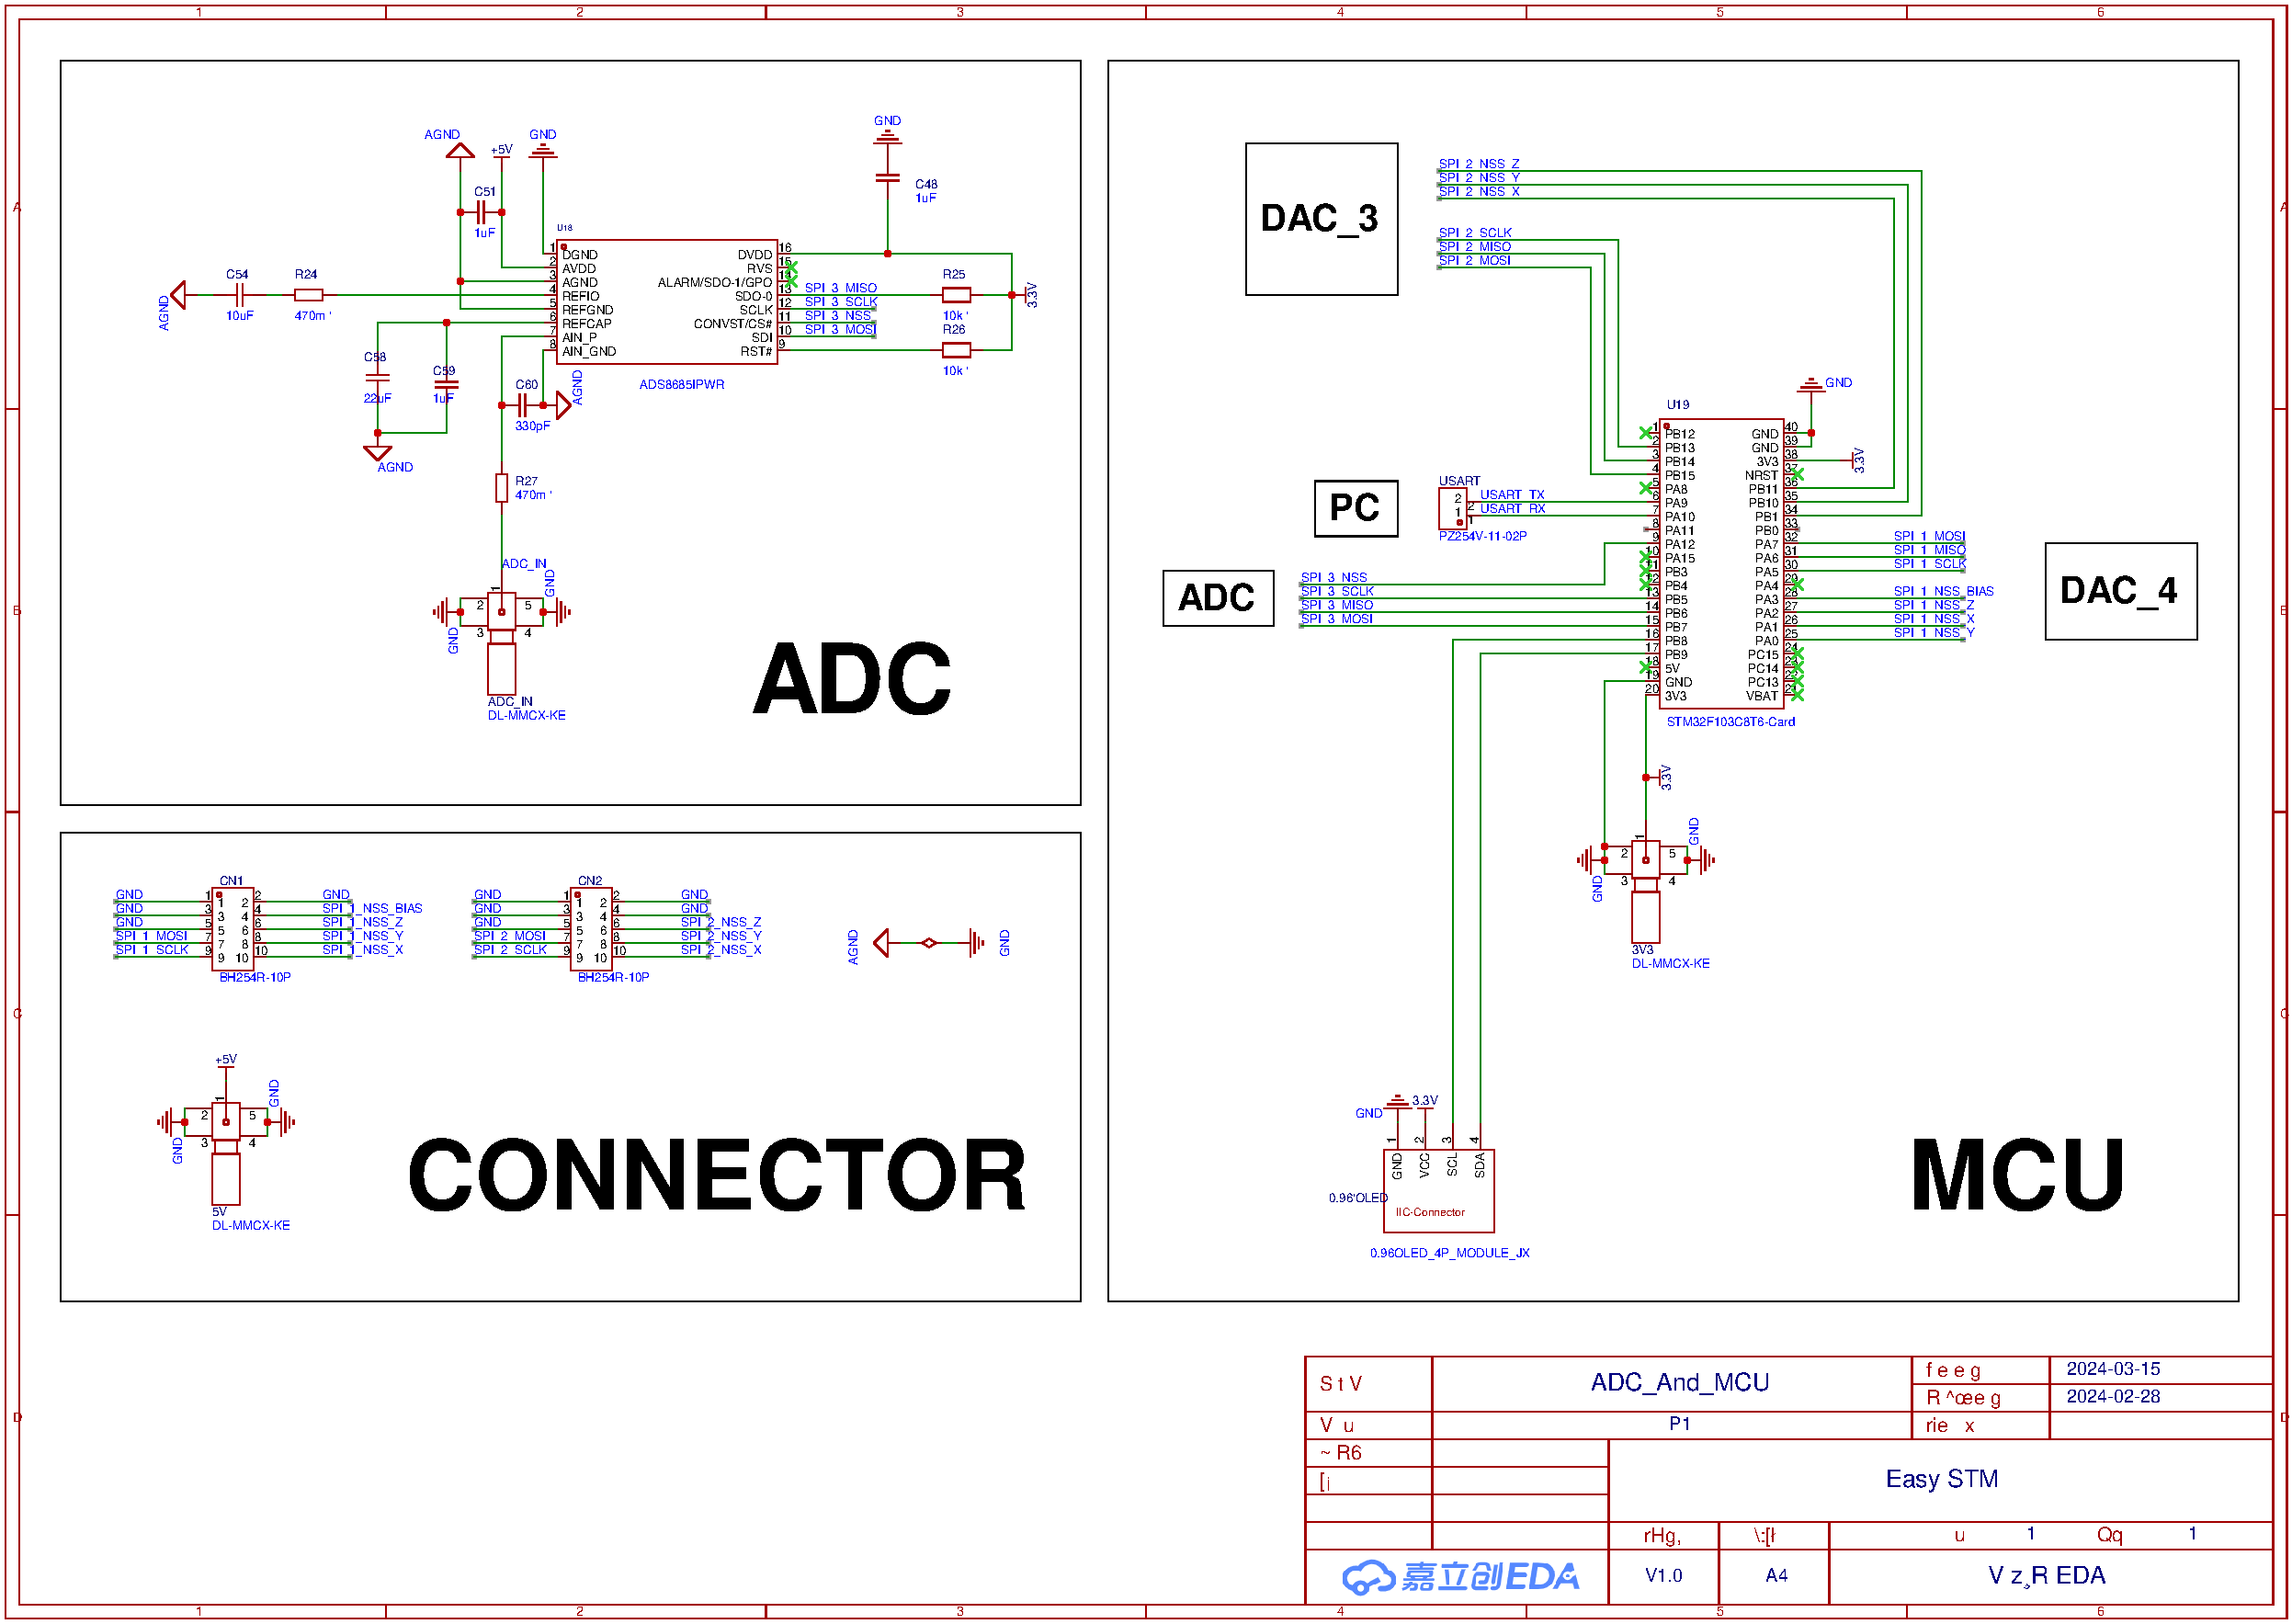
\includegraphics[width=\textwidth]{/PDF_Easy STM_2024-04-03/SCH_ADC_And_MCU_1-P1_2024-04-03.pdf}
		\caption{SCH\_ADC\_And\_MCU}
	\end{subfigure}
	\hfill
	\begin{subfigure}{0.47\textwidth}
		\centering
		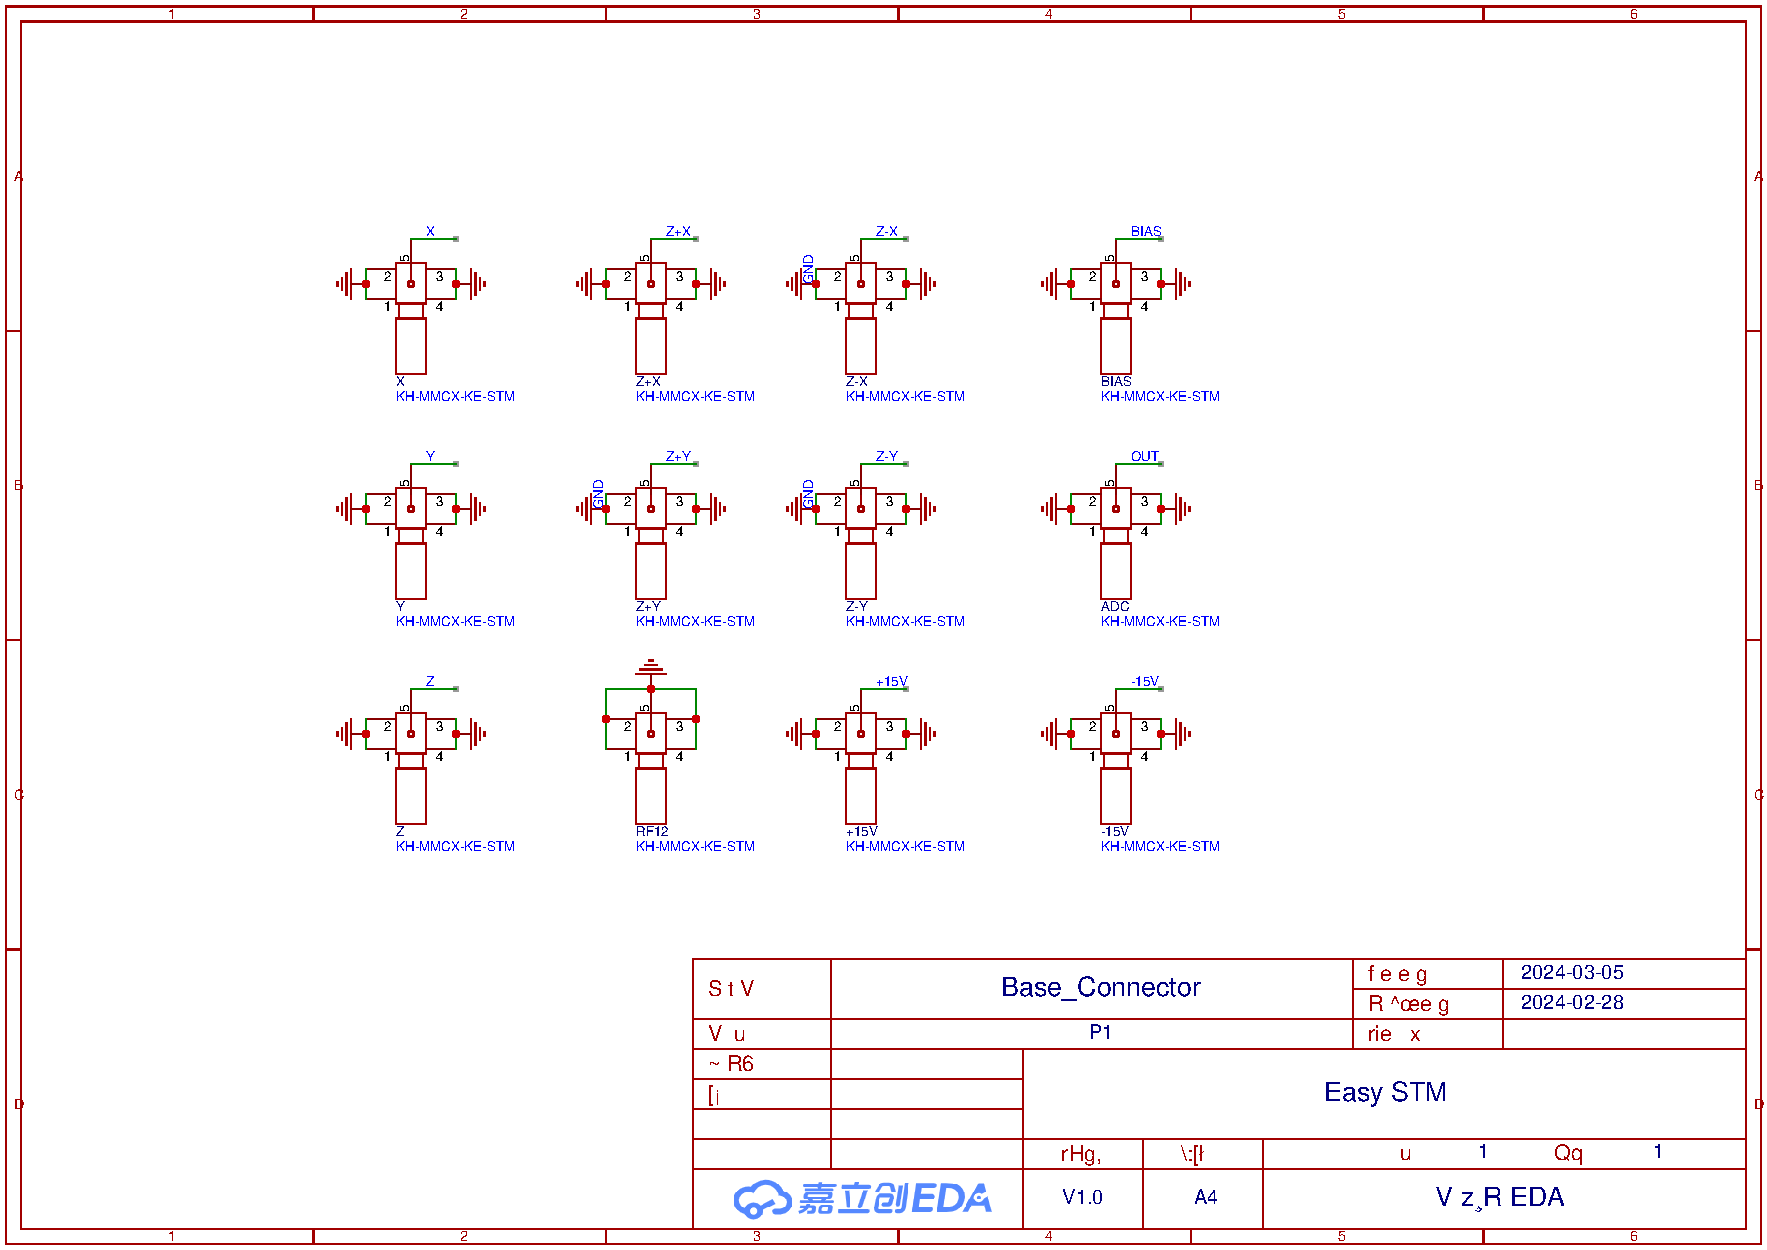
\includegraphics[width=\linewidth]{/PDF_Easy STM_2024-04-03/SCH_Base_Connector_1-P1_2024-04-03.pdf}
		\caption{SCH\_Base\_Connector}
	\end{subfigure}
	\hfill
	\vskip 1em
	\hfill
	\begin{subfigure}{0.47\textwidth}
		\centering
		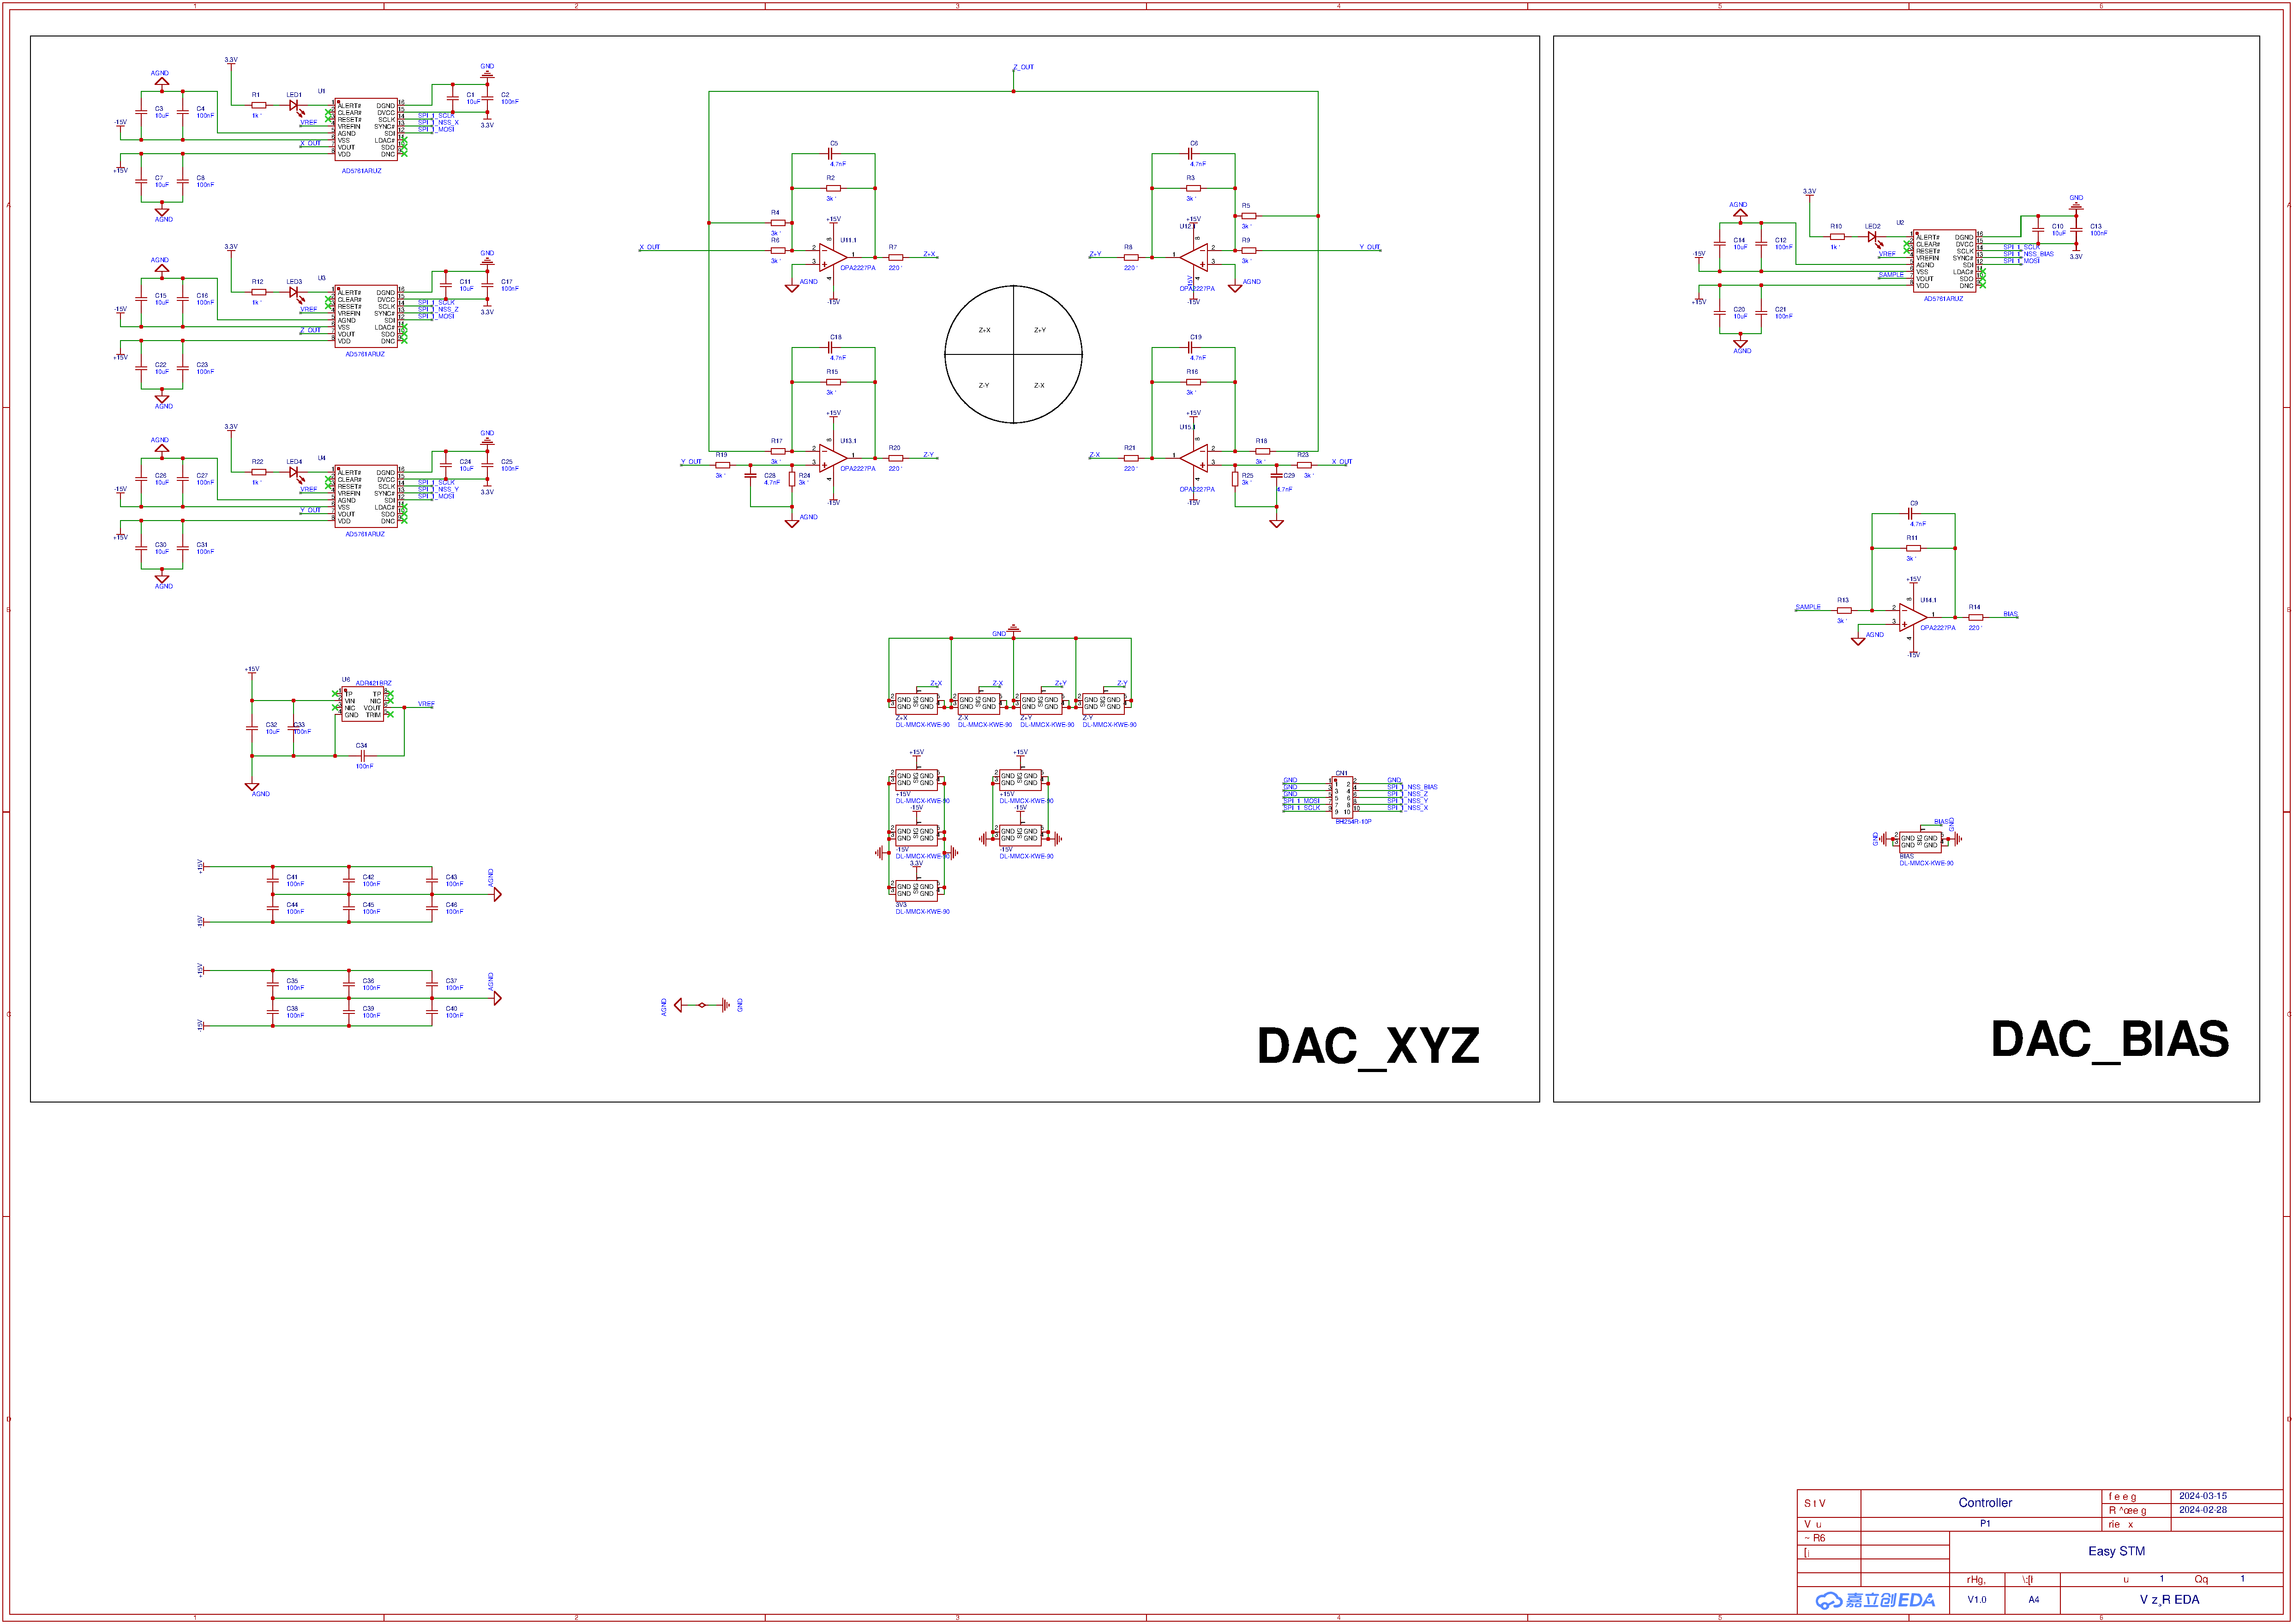
\includegraphics[width=\linewidth]{/PDF_Easy STM_2024-04-03/SCH_Controller_1-P1_2024-04-03.pdf}
		\caption{SCH\_Controller}
	\end{subfigure}
	\hfill
	\begin{subfigure}{0.47\textwidth}
		\centering
		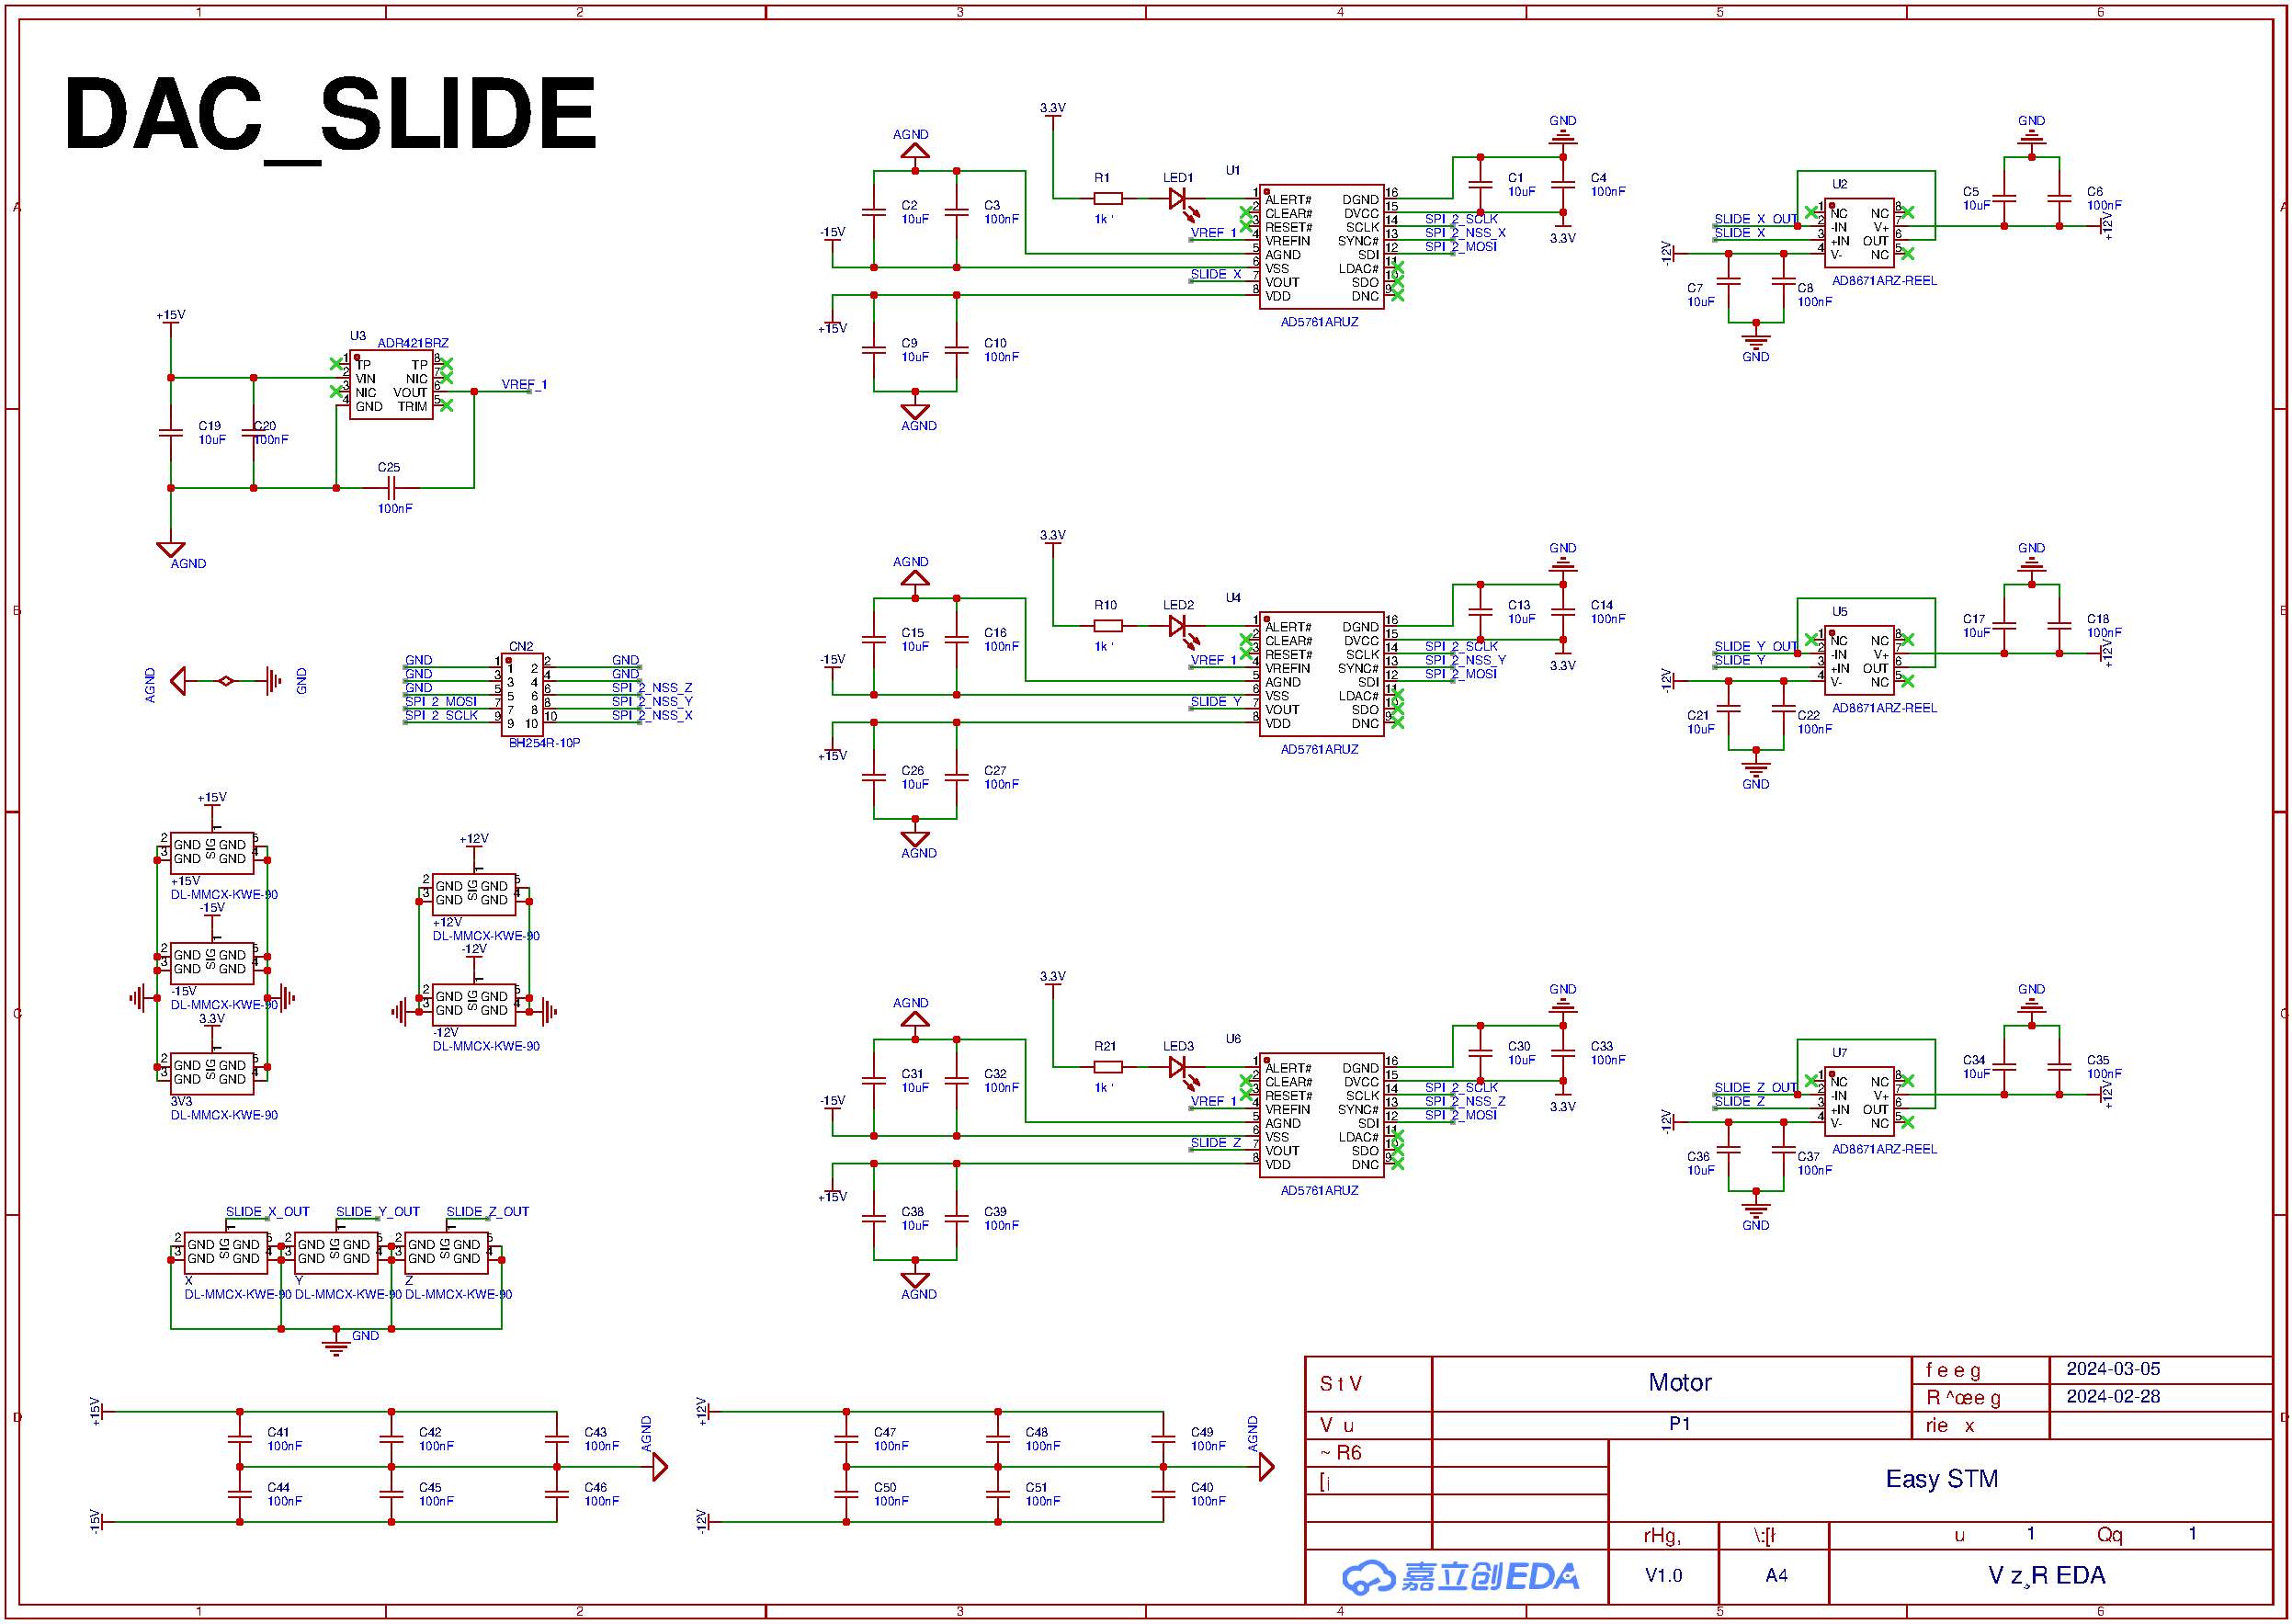
\includegraphics[width=\linewidth]{/PDF_Easy STM_2024-04-03/SCH_Motor_1-P1_2024-04-03.pdf}
		\caption{SCH\_Motor}
	\end{subfigure}
	\hfill
	\vskip 1em
	\hfill
	\begin{subfigure}{0.47\textwidth}
		\centering
		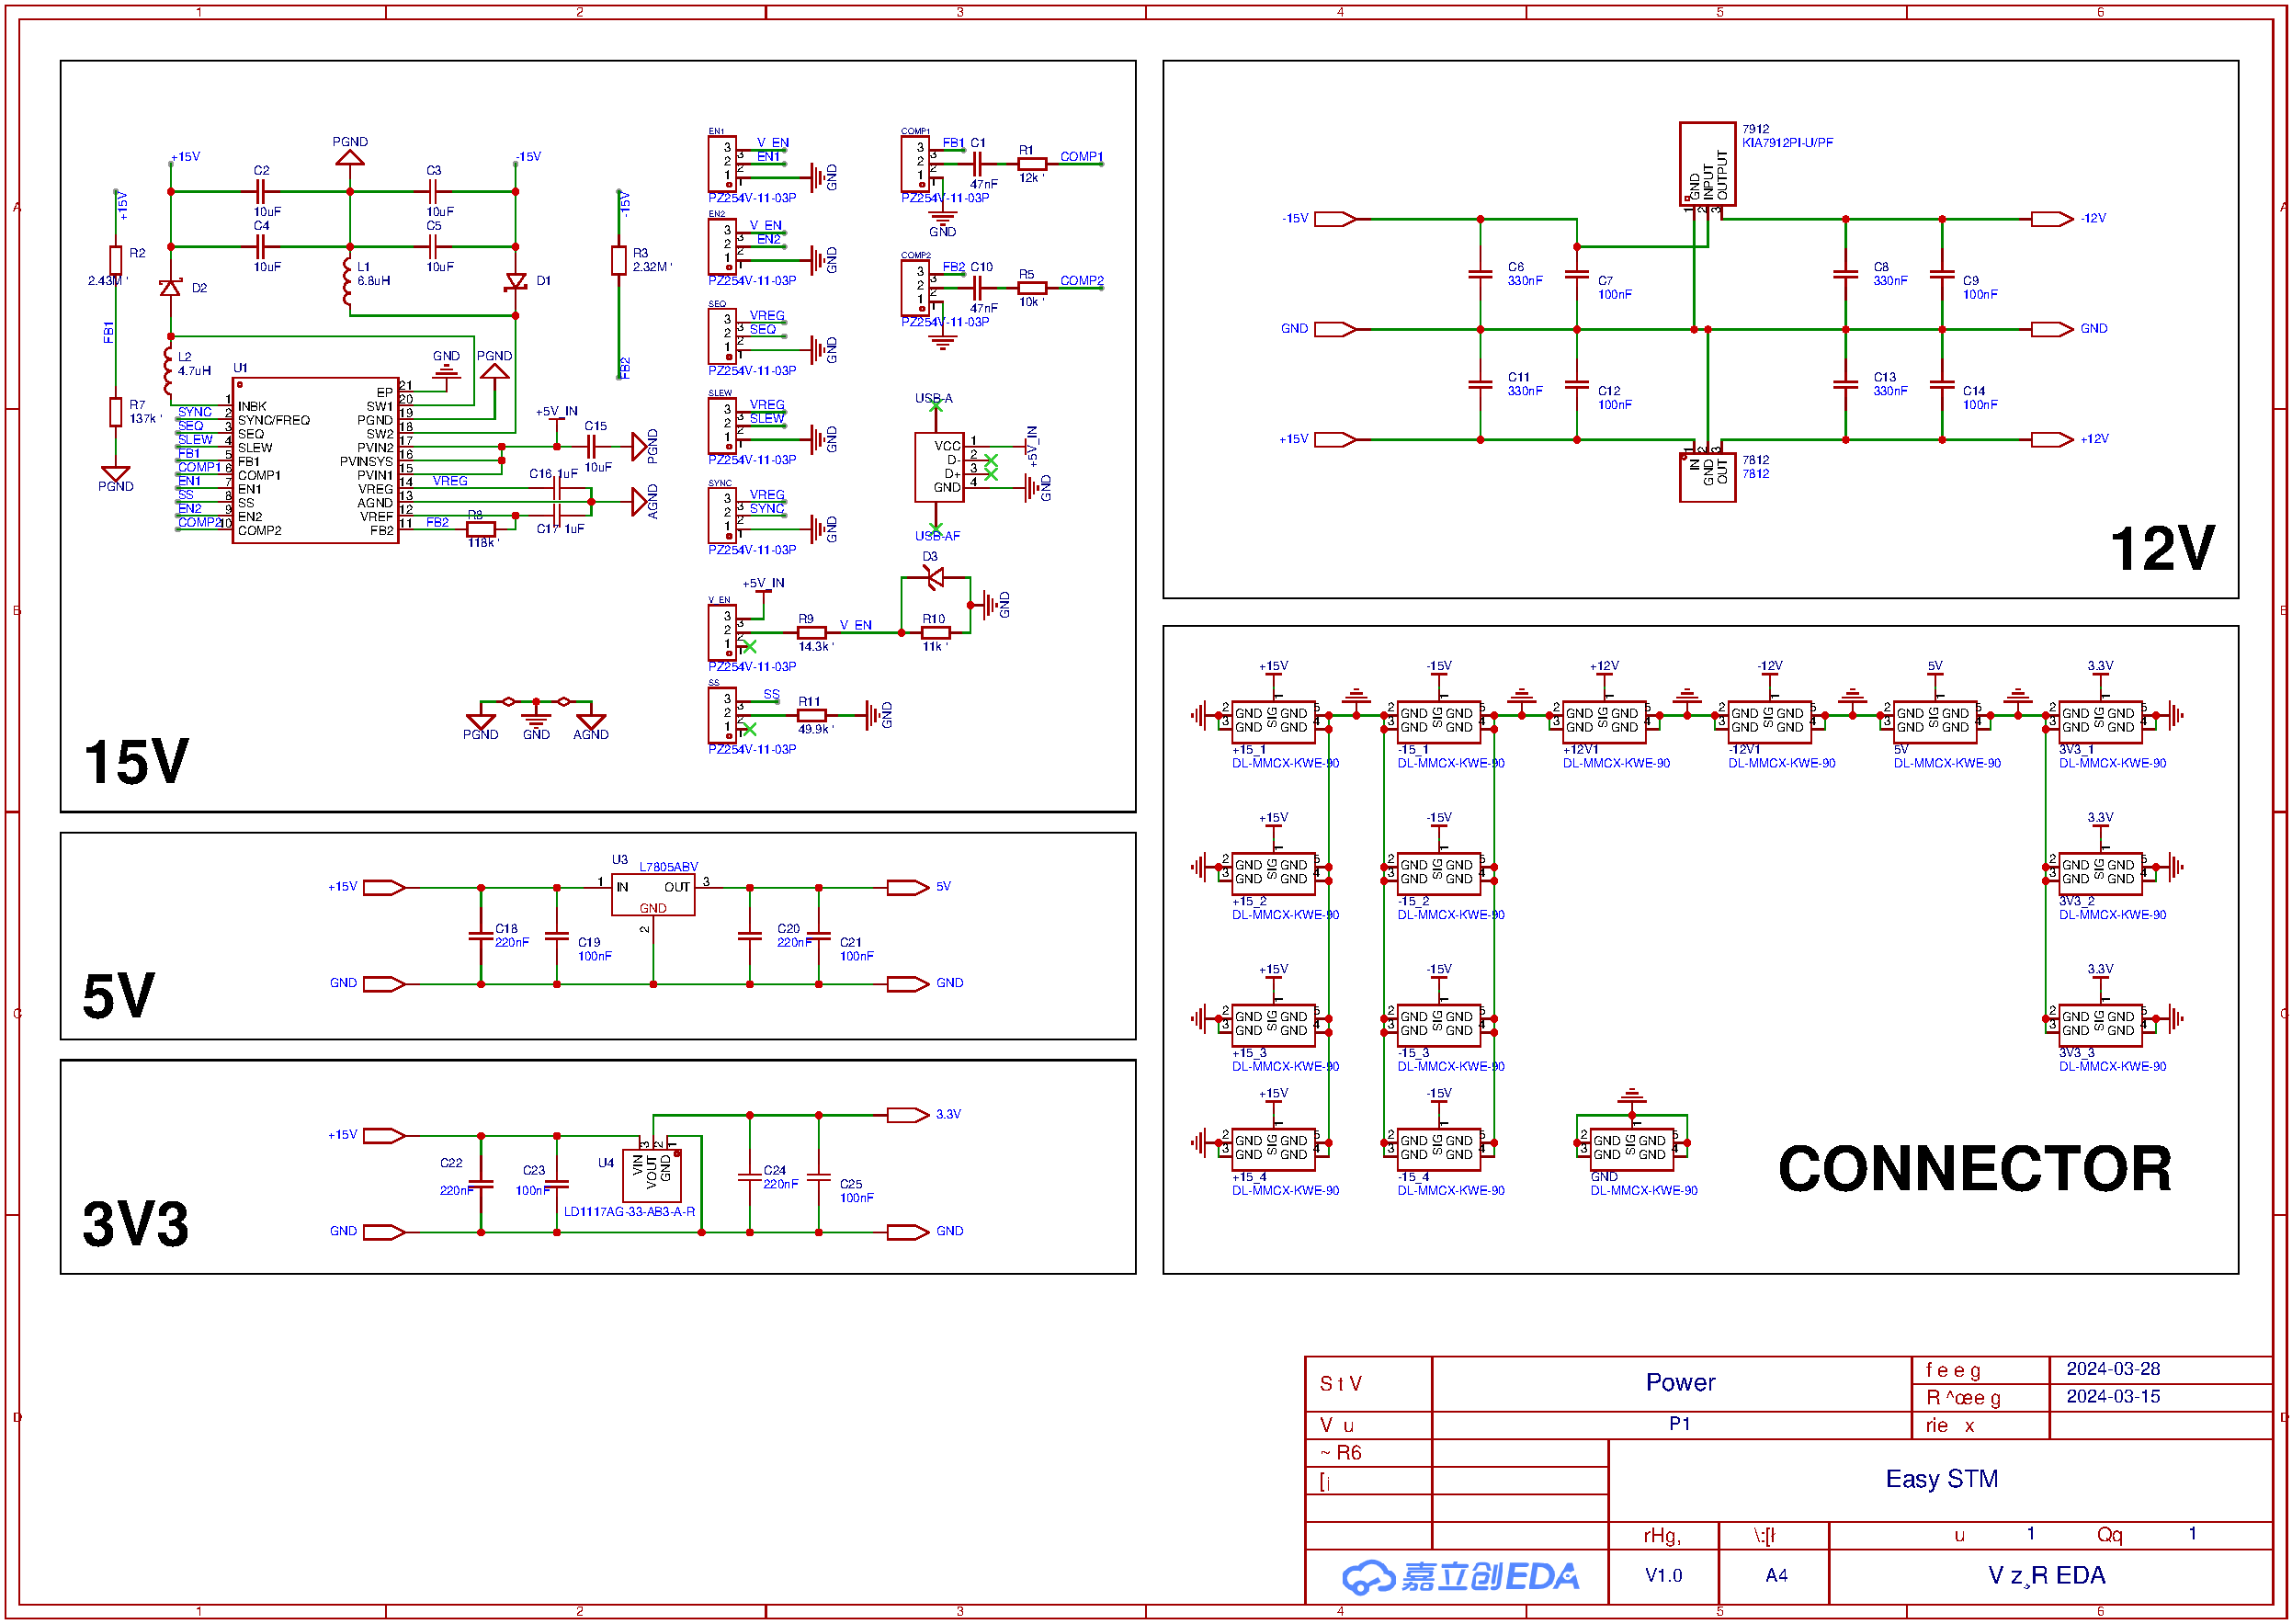
\includegraphics[width=\linewidth]{/PDF_Easy STM_2024-04-03/SCH_Power_1-P1_2024-04-03.pdf}
		\caption{SCH\_Power}
	\end{subfigure}
	\hfill
	\begin{subfigure}{0.47\textwidth}
		\centering
		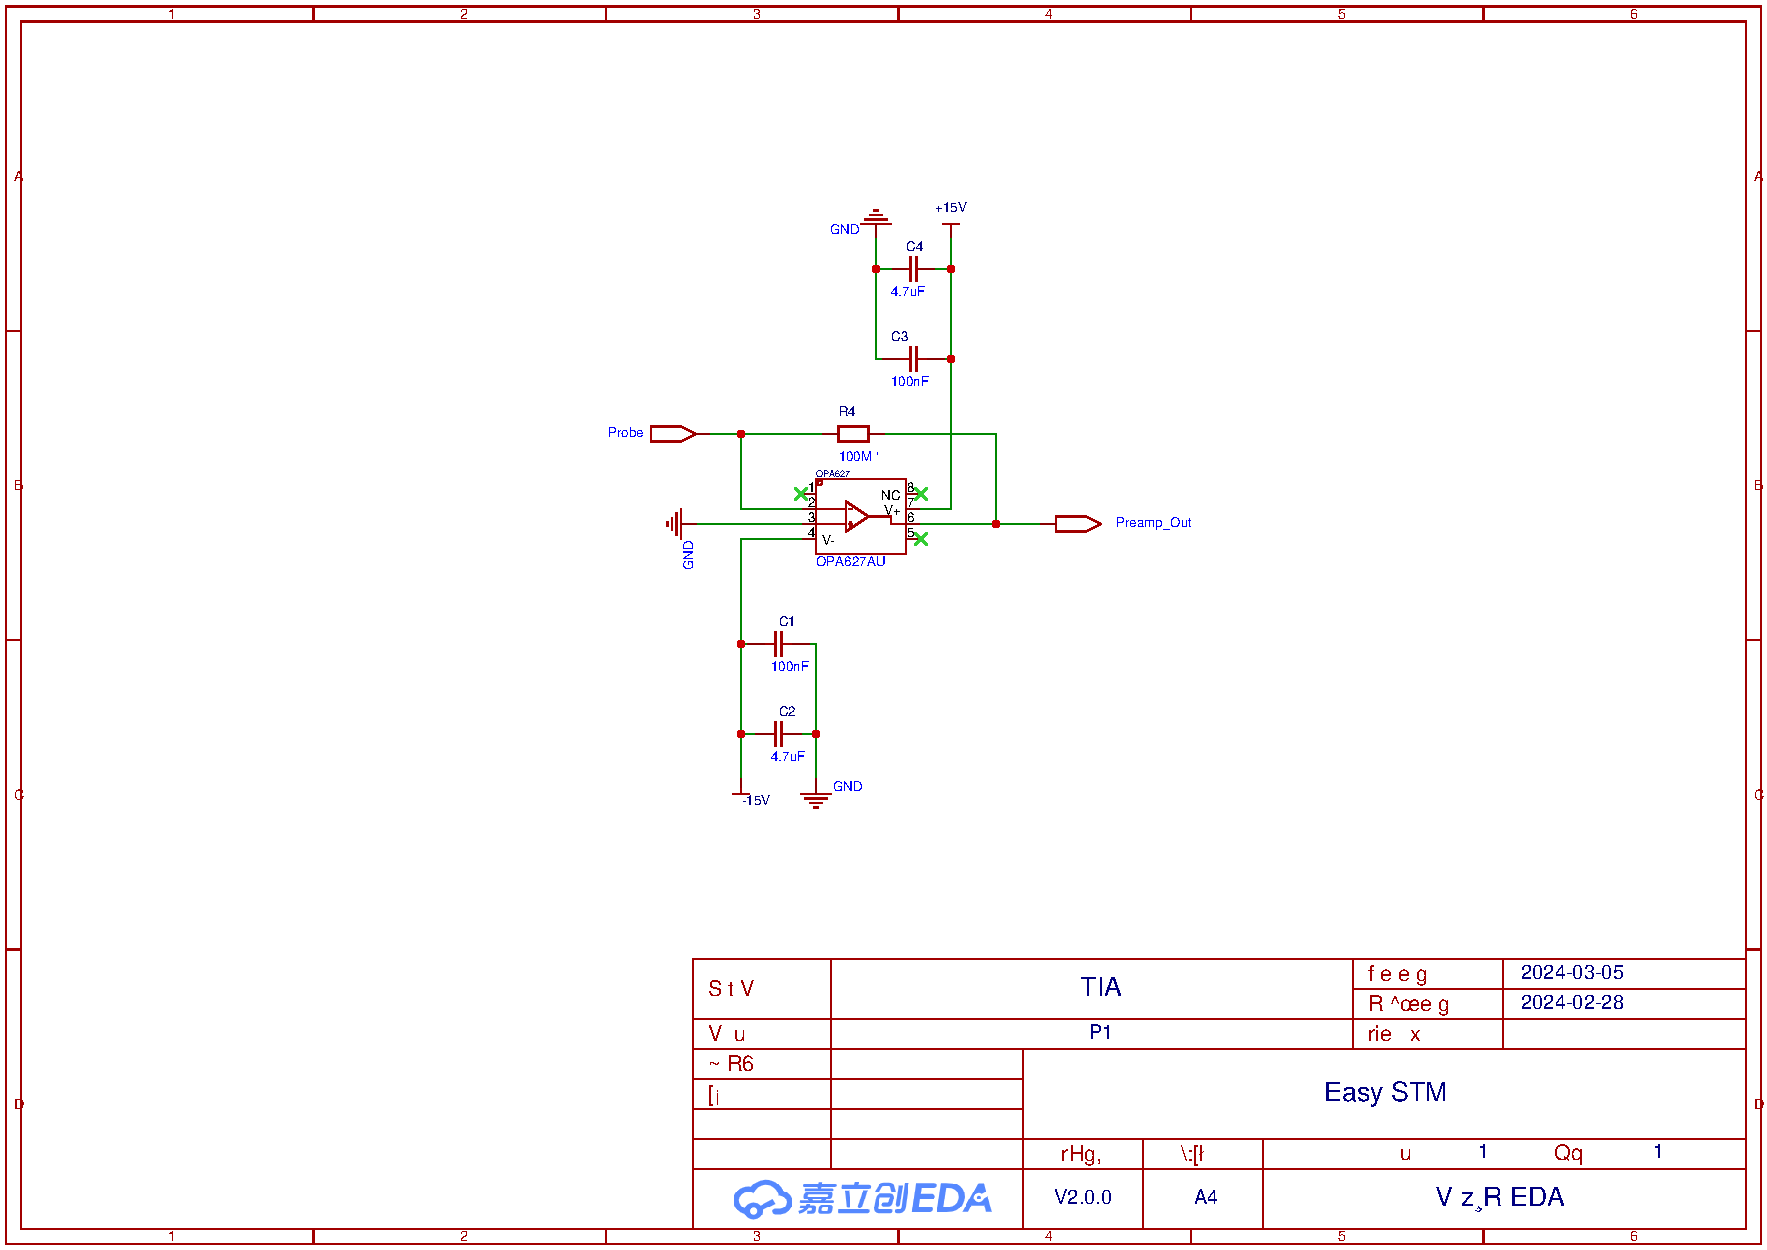
\includegraphics[width=\linewidth]{/PDF_Easy STM_2024-04-03/SCH_TIA_1-P1_2024-04-03.pdf}
		\caption{SCH\_TIA}
	\end{subfigure}
	\hfill
	\caption{主要 DIY-STM 电路原理图}
\end{figure}



\begin{figure}[!h]
	\centering
	\hfill
	\begin{subfigure}{0.47\textwidth}
		\centering
		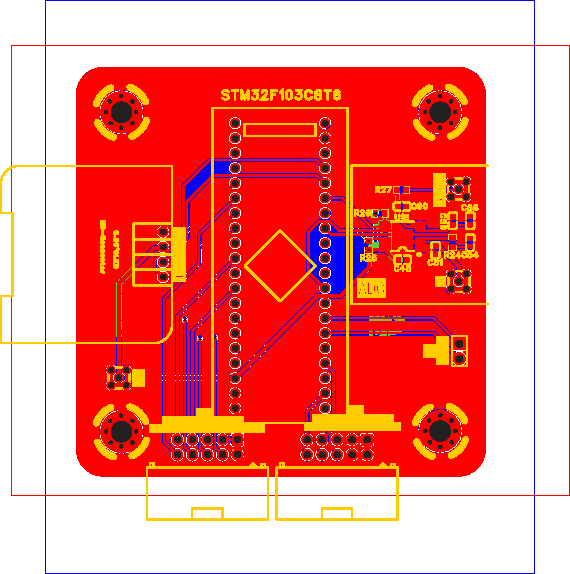
\includegraphics[width=\textwidth,clip,trim= 0 20 0 20]{/PCB/PCB_ADC_And_MCU_2024-04-04.pdf}
		\caption{PCB\_ADC\_And\_MCU}
	\end{subfigure}
	\hfill
	\begin{subfigure}{0.47\textwidth}
		\centering
		\vfill
		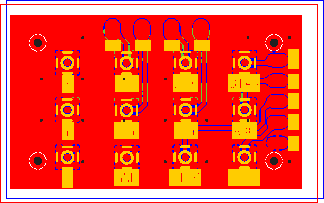
\includegraphics[width=\linewidth]{/PCB/PCB_Base_Connector_2024-04-04.pdf}
		\vfill
		\caption{PCB\_Base\_Connector}
	\end{subfigure}
	\hfill
	\vskip 1em
	\hfill
	\begin{subfigure}{0.47\textwidth}
		\centering
		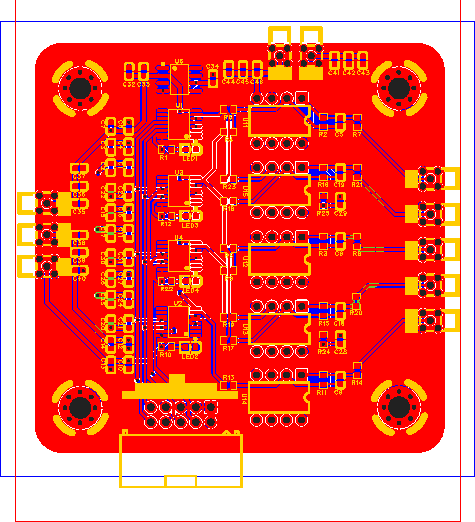
\includegraphics[width=\linewidth,clip,trim= -20 0 -22 0]{/PCB/PCB_Controller_2024-04-04.pdf}
		\caption{PCB\_Controller}
	\end{subfigure}
	\hfill
	\begin{subfigure}{0.47\textwidth}
		\centering
		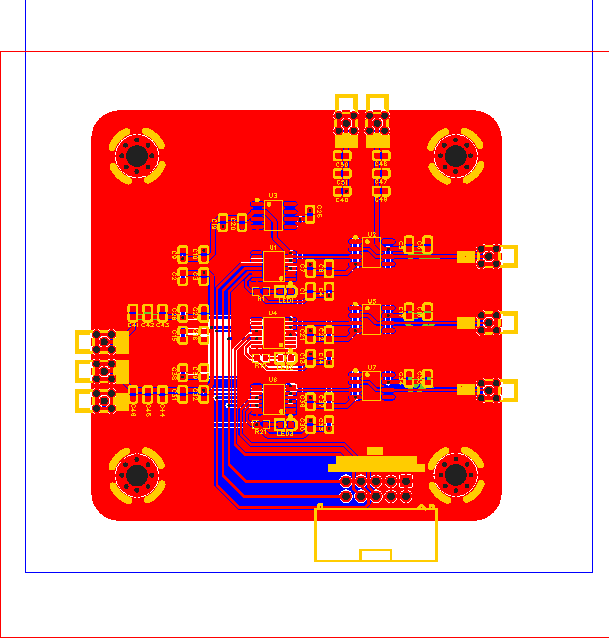
\includegraphics[width=\linewidth,clip,trim= 10 22 10 40]{/PCB/PCB_Motor_2024-04-04.pdf}
		\caption{PCB\_Motor}
	\end{subfigure}
	\hfill
	\vskip 1em
	\hfill
	\begin{subfigure}{0.47\textwidth}
		\centering
		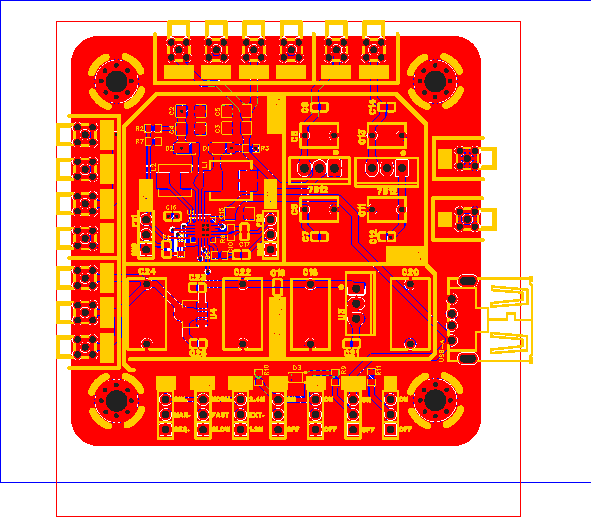
\includegraphics[width=\linewidth,clip,trim= 0 20 20 0]{/PCB/PCB_Power_2024-04-04.pdf}
		\caption{PCB\_Power}
	\end{subfigure}
	\hfill
	\begin{subfigure}{0.47\textwidth}
		\centering
		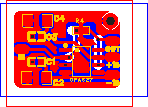
\includegraphics[width=\linewidth,clip,trim= 0 0 5 0]{/PCB/PCB_TIA_2024-04-04.pdf}
		\caption{PCB\_TIA}
	\end{subfigure}
	\hfill
	\caption{主要 DIY-STM PCB 设计图}
\end{figure}


\clearpage
\section*{附录 B\quad 示例代码}
\phantomsection
\addcontentsline{toc}{section}{附录 B\quad 示例代码} % 将无标号章节添加至目录
\label{app:B}

\lstset{language=Python}	%代码语言
\lstset{breaklines}			%自动将长的代码行换行排版

\lstset{caption={PID 控制恒流模式 Python 代码}}
\begin{lstlisting}
	import time
	import matplotlib.pyplot as plt
	import math
	
	# PID控制器参数
	Kp = 1.0
	Ki = 0.2
	Kd = 5.0
	
	# 初始化全局变量
	setpoint = 1.0  # 目标隧穿电流
	integral = 0.0  # 积分项初始化
	previous_time = time.time()  # 上次控制时间初始化
	sample_time = 0.2  # 控制循环的时间间隔,单位:秒
	previous_error = 0.0  # 初始化previous_error
	max_runtime = 10  # 最大运行时间,单位:秒
	
	# 用于记录数据的列表
	measurements = []
	pid_outputs = []
	times = []
	
	# 假设的测量和调整函数
	def measure_current():
	# 测量隧穿电流
	# 这里模拟一个正弦波电流,用于演示
	return 0.5 + 0.2 * math.sin(2 * math.pi * time.time())
	
	def adjust_probe(position):
	# 调整探针位置
	# 这里记录PID输出值,用于后续绘图
	pid_outputs.append(position)
	
	def pid_controller():
	global integral, previous_time, previous_error
	current_time = time.time()
	if current_time - previous_time >= max_runtime: # 检查运行时间是否超过最大运行时间
	return False
	measured_current = measure_current()
	error = setpoint - measured_current # 计算误差
	integral = min(max(integral + error * sample_time, -100), 100)  # 计算积分项,限制在-100到100
	derivative = (error - previous_error) / sample_time if previous_time != 0 else 0    # 计算微分项
	previous_error = error
	output = Kp * error + Ki * integral + Kd * derivative   # 计算PID输出
	output = max(min(output, 100.0), -100.0)  # PID输出限制在-100到100
	adjust_probe(output)    # 调整探针位置
	measurements.append(measured_current)   # 记录数据
	times.append(current_time - previous_time)
	return True
	
	# 主函数
	def main():
	try:
	while pid_controller():  # 调用PID控制器,根据返回值决定是否继续循环
	time.sleep(sample_time)  # 等待指定的采样时间
	except KeyboardInterrupt:
	print("用户中断了PID控制器。")
	finally:
	# 绘制测量电流随时间变化的图表
	plt.figure(figsize=(10, 5))
	plt.plot(times, measurements, label='Measured Current')
	plt.xlabel('Time (s)')
	plt.ylabel('Current')
	plt.title('Measured Current Over Time')
	plt.legend()
	plt.show()
	
	# 绘制PID控制器输出随时间变化的图表
	plt.figure(figsize=(10, 5))
	plt.plot(times, pid_outputs, label='PID Output', color='r')
	plt.xlabel('Time (s)')
	plt.ylabel('PID Output')
	plt.title('PID Output Over Time')
	plt.legend()
	plt.show()
	
	if __name__ == "__main__":
	main()
\end{lstlisting}

\clearpage
\lstset{caption={对数拟合算法示例代码}}
\begin{lstlisting}
	import numpy as np
	import matplotlib.pyplot as plt
	from scipy.optimize import curve_fit
	
	# 生成模拟数据
	x = np.linspace(1, 10, 50)
	y = 100 * np.exp(-0.1 * x)  # 使用对数函数生成数据
	y_noisy = y + np.random.normal(0, 5, x.shape)	# 添加一些噪声
	
	# 定义对数函数模型
	def log_model(x, a, b):
	return a * np.log(x) + b
	
	# 使用curve_fit进行曲线拟合
	popt, pcov = curve_fit(log_model, x, y_noisy)
	
	# 使用拟合参数生成拟合曲线
	x_fit = np.linspace(1, 10, 200)
	y_fit = log_model(x_fit, *popt)
	
	# 绘制原始数据和拟合曲线
	plt.figure(figsize=(10, 6))
	plt.scatter(x, y_noisy, label='Noisy Data', color='blue', alpha=0.5)
	plt.plot(x_fit, y_fit, label='Fitted Curve', color='red')
	plt.xlabel('X-axis')
	plt.ylabel('Y-axis')
	plt.title('Logarithmic Curve Fitting')
	plt.legend()
	plt.show()
\end{lstlisting}

\clearpage
\lstset{caption={二维图像重建算法示例代码}}
\begin{lstlisting}
	import numpy as np
	import matplotlib.pyplot as plt
	
	np.random.seed(0)	# 设置随机种子以获得可重复的结果
	n_points = 1000		# 定义数据点的数量
	
	# 生成线性分布的x和y坐标
	x = np.linspace(0, 10 * np.pi, n_points)
	y = np.linspace(0, 10 * np.pi, n_points)
	XX, YY = np.meshgrid(x, y)
	
	# 生成模拟数据
	Z = np.sin(XX) + np.sin(YY)	# 生成正弦波数据
	noise = np.random.normal(0, 0.2, (n_points, n_points))
	Z_noisy = Z + noise			# 添加噪声
	
	# 创建一个新的图形窗口
	plt.figure(figsize=(10, 8))
	
	# 绘制带有噪声的正弦波
	plt.contourf(XX, YY, Z_noisy, cmap='viridis', levels=20)
	plt.colorbar(label='Height')
	plt.title('Surface Image in 2D')
	plt.xlabel('X Axis')
	plt.ylabel('Y Axis')
	
	# 显示网格
	plt.grid(True)
	plt.show()
\end{lstlisting}


\clearpage
\lstset{caption={三维图像重建算法示例代码}}
\begin{lstlisting}
	import numpy as np
	import matplotlib.pyplot as plt
	from mpl_toolkits.mplot3d import Axes3D
	
	np.random.seed(0)	# 设置随机种子以获得可重复的结果
	n_points = 100		# 定义数据点的数量
	
	# 生成线性分布的数据点
	x = np.linspace(0, 5 * np.pi, n_points)
	y = np.linspace(0, 5 * np.pi, n_points)
	z = np.linspace(0, 0.3, n_points)
	
	# 生成网格
	X, Y = np.meshgrid(x, y)
	Z = np.sin(X) * np.cos(Y)
	
	# 添加噪声
	noise = np.random.normal(0, 0.1, (n_points, n_points))
	Z_noisy = Z + noise
	
	# 创建一个新的图形窗口
	fig = plt.figure(figsize=(10, 8))
	
	# 添加一个3D subplot
	ax = fig.add_subplot(111, projection='3d')
	
	# 绘制带有噪声的三维散点图
	ax.scatter(X, Y, Z_noisy, c=Z_noisy, cmap='viridis', s=5)
	
	# 添加颜色条
	ax.figure.colorbar(ax.scatter(X, Y, Z_noisy, c=Z_noisy, cmap='viridis', s=5), label='Height')
	
	# 设置标题和轴标签
	ax.set_title('Surface Image in 3D')
	ax.set_xlabel('X Axis')
	ax.set_ylabel('Y Axis')
	ax.set_zlabel('Z Axis')
	
	# 显示图形
	plt.show()
\end{lstlisting}
%====================附录====================
	
	
\end{document}
% You have reached the end of world.